% Power-board random vibration | report issued 5 October 2026.
% Figures are ordinary external graphics in the figures/ directory.
% Random-vibration results from 5 October 2026.
\documentclass[10pt,a4paper]{article}
\usepackage[margin=18mm,headheight=14pt,headsep=7mm,footskip=10mm]{geometry}
\usepackage{iftex}
\ifPDFTeX
  \usepackage[T1]{fontenc}
  \usepackage[utf8]{inputenc}
\fi
\usepackage{lmodern,amsmath,graphicx,booktabs,array,caption,xcolor,fancyhdr,hyperref}
\definecolor{Navy}{HTML}{17354B}
\definecolor{Teal}{HTML}{166979}
\hypersetup{colorlinks=true,urlcolor=Teal,linkcolor=Teal,
 pdftitle={Power board: random vibration},
 pdfauthor={MIT Rocket Team -- simulation study}}
\captionsetup{font=small,labelfont=bf,justification=raggedright,singlelinecheck=false,hypcap=false}
\pagestyle{fancy}\fancyhf{}
\fancyhead[L]{\small\color{Navy}MIT Rocket Team \enspace | \enspace Power board}
\fancyhead[R]{\small\color{Navy}Random vibration}
\fancyfoot[L]{\footnotesize Report issued 5 October 2026}
\fancyfoot[R]{\footnotesize\thepage}
\renewcommand{\headrulewidth}{0.3pt}
\setlength{\parindent}{0pt}\setlength{\parskip}{5pt}
\setlength{\emergencystretch}{2em}
\renewcommand{\arraystretch}{1.07}
\newcommand{\ReportHeading}[1]{\par\vspace{7pt}{\large\bfseries\color{Teal}#1}\par\vspace{3pt}}
\newcommand{\PageTitle}[1]{{\LARGE\bfseries\color{Navy}#1\par}\vspace{7pt}}
\usepackage{pgfplots}\pgfplotsset{compat=1.18}
\newcommand{\ReportBody}{%
\PageTitle{Power board: random vibration}
{\large\color{Teal}Separate X, Y and Z base excitation \enspace | \enspace 2\% assumed damping}\par
{\small Six locked bolts at 750 N each. ANSYS Mechanical/MAPDL 2026 R1.02.}\par
Three separate random-vibration analyses of the complete populated assembly were completed using the supplied 20--2000 Hz acceleration PSD and an exploratory constant modal damping ratio of 2\%. The model inherits the converged, locked six-bolt state from the 750 N-per-bolt static study. The calculated response uses all 38 prestressed modes between 485.964 and 3986.075 Hz.

The largest PCB directional displacement RMS is 0.052674 mm under Z-axis excitation. The greatest PCB equivalent-stress RMS is 90.325 MPa under X-axis excitation. Results below are separate directional load cases; they are not a simultaneous three-axis environment.

\ReportHeading{PCB random-response RMS}
\begin{center}
\begin{tabular}{c r c r}
\toprule
\textbf{Base axis} & \textbf{Max component u (mm)} & \textbf{Component} & \textbf{PCB stress (MPa)} \\
\midrule
X & 0.023366 & Z & 90.325 \\
Y & 0.01945 & Z & 17.85 \\
Z & 0.052674 & Z & 32.482 \\
\bottomrule
\end{tabular}
\end{center}
Displacements are relative to the mounting supports. Stress is the unaveraged Segalman--Fulcher equivalent-stress RMS, excluding the static mean stress. These exploratory elastic values are not a pass/fail strength assessment.

\textbf{Interpretation:} The highest whole-assembly elastic equivalent-stress RMS is 1443.2 MPa under X-axis excitation. The localized hardware maxima require mesh, connection and material validation; numerical completion is not evidence of structural adequacy.

\ReportHeading{Specified acceleration spectrum}
\begin{center}\begin{minipage}[c]{.32\linewidth}
\begin{center}
\begin{tabular}{r r}
\toprule
\textbf{Hz} & \textbf{PSD (g$^2$/Hz)} \\
\midrule
20 & 0.026 \\
50 & 0.16 \\
800 & 0.16 \\
2000 & 0.026 \\
\bottomrule
\end{tabular}
\end{center}
\end{minipage}\hfill\begin{minipage}[c]{.65\linewidth}% Editable native PGFPlots figure. Four user-specified PSD points.
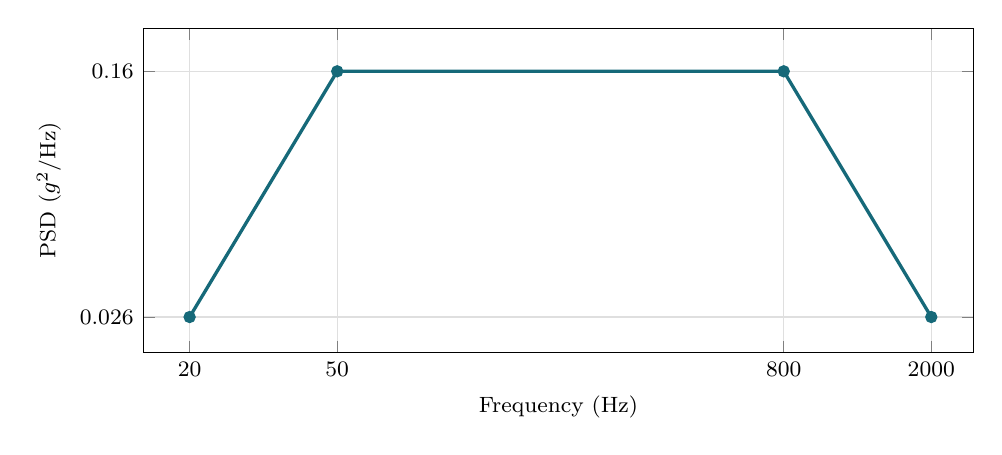
\begin{tikzpicture}
\begin{loglogaxis}[
 width=\linewidth,height=5.7cm,
 xmin=15,xmax=2600,ymin=0.02,ymax=0.22,
 xlabel={Frequency (Hz)},ylabel={PSD ($g^2$/Hz)},
 xtick={20,50,800,2000},xticklabels={20,50,800,2000},
 ytick={0.026,0.16},yticklabels={0.026,0.16},
 grid=both,major grid style={gray!25},minor grid style={gray!12},
 tick label style={font=\footnotesize},label style={font=\footnotesize},
 scaled ticks=false]
\addplot[color=Teal,line width=1.2pt,mark=*,mark size=1.6pt]
 coordinates {(20,0.026) (50,0.16) (800,0.16) (2000,0.026)};
\end{loglogaxis}
\end{tikzpicture}
\end{minipage}
\captionof{figure}{Specified PSD with power-law interpolation between the supplied points. Integrated input: 14.136 g RMS.}\end{center}
The Mechanical load panel may display 15.310 g RMS because its display uses a linear trapezoidal integral of the four points. The piecewise log-log spectrum integrates to 14.136 g RMS; no input points were changed.

\clearpage\PageTitle{Directional response results}
\ReportHeading{PCB directional displacement RMS (mm)}
\begin{center}
\begin{tabular}{c r r r}
\toprule
\textbf{Base axis} & \textbf{X response} & \textbf{Y response} & \textbf{Z response} \\
\midrule
X & 0.002806 & 0.00069972 & 0.023366 \\
Y & 0.00033604 & 0.00095143 & 0.01945 \\
Z & 0.0016244 & 0.0023607 & 0.052674 \\
\bottomrule
\end{tabular}
\end{center}
\ReportHeading{PCB absolute acceleration RMS (g)}
\begin{center}
\begin{tabular}{c r r r}
\toprule
\textbf{Base axis} & \textbf{X response} & \textbf{Y response} & \textbf{Z response} \\
\midrule
X & 15.282 & 1.9137 & 52.287 \\
Y & 0.98316 & 16.735 & 31.582 \\
Z & 4.6891 & 4.8063 & 154.66 \\
\bottomrule
\end{tabular}
\end{center}
\ReportHeading{Whole-assembly directional displacement RMS (mm)}
\begin{center}
\begin{tabular}{c r r r}
\toprule
\textbf{Base axis} & \textbf{X response} & \textbf{Y response} & \textbf{Z response} \\
\midrule
X & 0.061425 & 0.0038971 & 0.028948 \\
Y & 0.001215 & 0.012275 & 0.029746 \\
Z & 0.014838 & 0.033204 & 0.0806 \\
\bottomrule
\end{tabular}
\end{center}
\ReportHeading{Whole-assembly absolute acceleration RMS (g)}
\begin{center}
\begin{tabular}{c r r r}
\toprule
\textbf{Base axis} & \textbf{X response} & \textbf{Y response} & \textbf{Z response} \\
\midrule
X & 103.5 & 10.503 & 52.287 \\
Y & 8.9608 & 22.867 & 31.582 \\
Z & 50.032 & 36.436 & 154.66 \\
\bottomrule
\end{tabular}
\end{center}
\ReportHeading{Stress and PCB strain}
\begin{center}
\begin{tabular}{c r r}
\toprule
\textbf{Base axis} & \textbf{PCB stress (MPa)} & \textbf{Assembly stress (MPa)} \\
\midrule
X & 90.325 & 1443.2 \\
Y & 17.85 & 29.288 \\
Z & 32.482 & 71.387 \\
\bottomrule
\end{tabular}
\end{center}
\begin{center}
\begin{tabular}{c r r r}
\toprule
\textbf{Base axis} & \textbf{PCB strain X ($\mu\varepsilon$)} & \textbf{Y ($\mu\varepsilon$)} & \textbf{Z ($\mu\varepsilon$)} \\
\midrule
X & 2216.1 & 771.68 & 3044.7 \\
Y & 200.71 & 353.58 & 389.94 \\
Z & 1116.9 & 952.02 & 720.88 \\
\bottomrule
\end{tabular}
\end{center}
Each table entry is a spatial maximum for that component; maxima need not occur at the same node. No vector sum of directional RMS maxima is reported. Three times a directional RMS value is a conventional 3-sigma estimate under a Gaussian assumption, not a guaranteed mission maximum. Equivalent stress is not Gaussian.

\clearpage\PageTitle{Whole-assembly response: X and Y excitation}
The solved model contains 208 meshed, unsuppressed bodies, including 172 imported electronic-component bodies. Every body has finite response values in all three cases. The PCB-only figures later in this report are scoped views of this same assembled solution.

\begin{center}
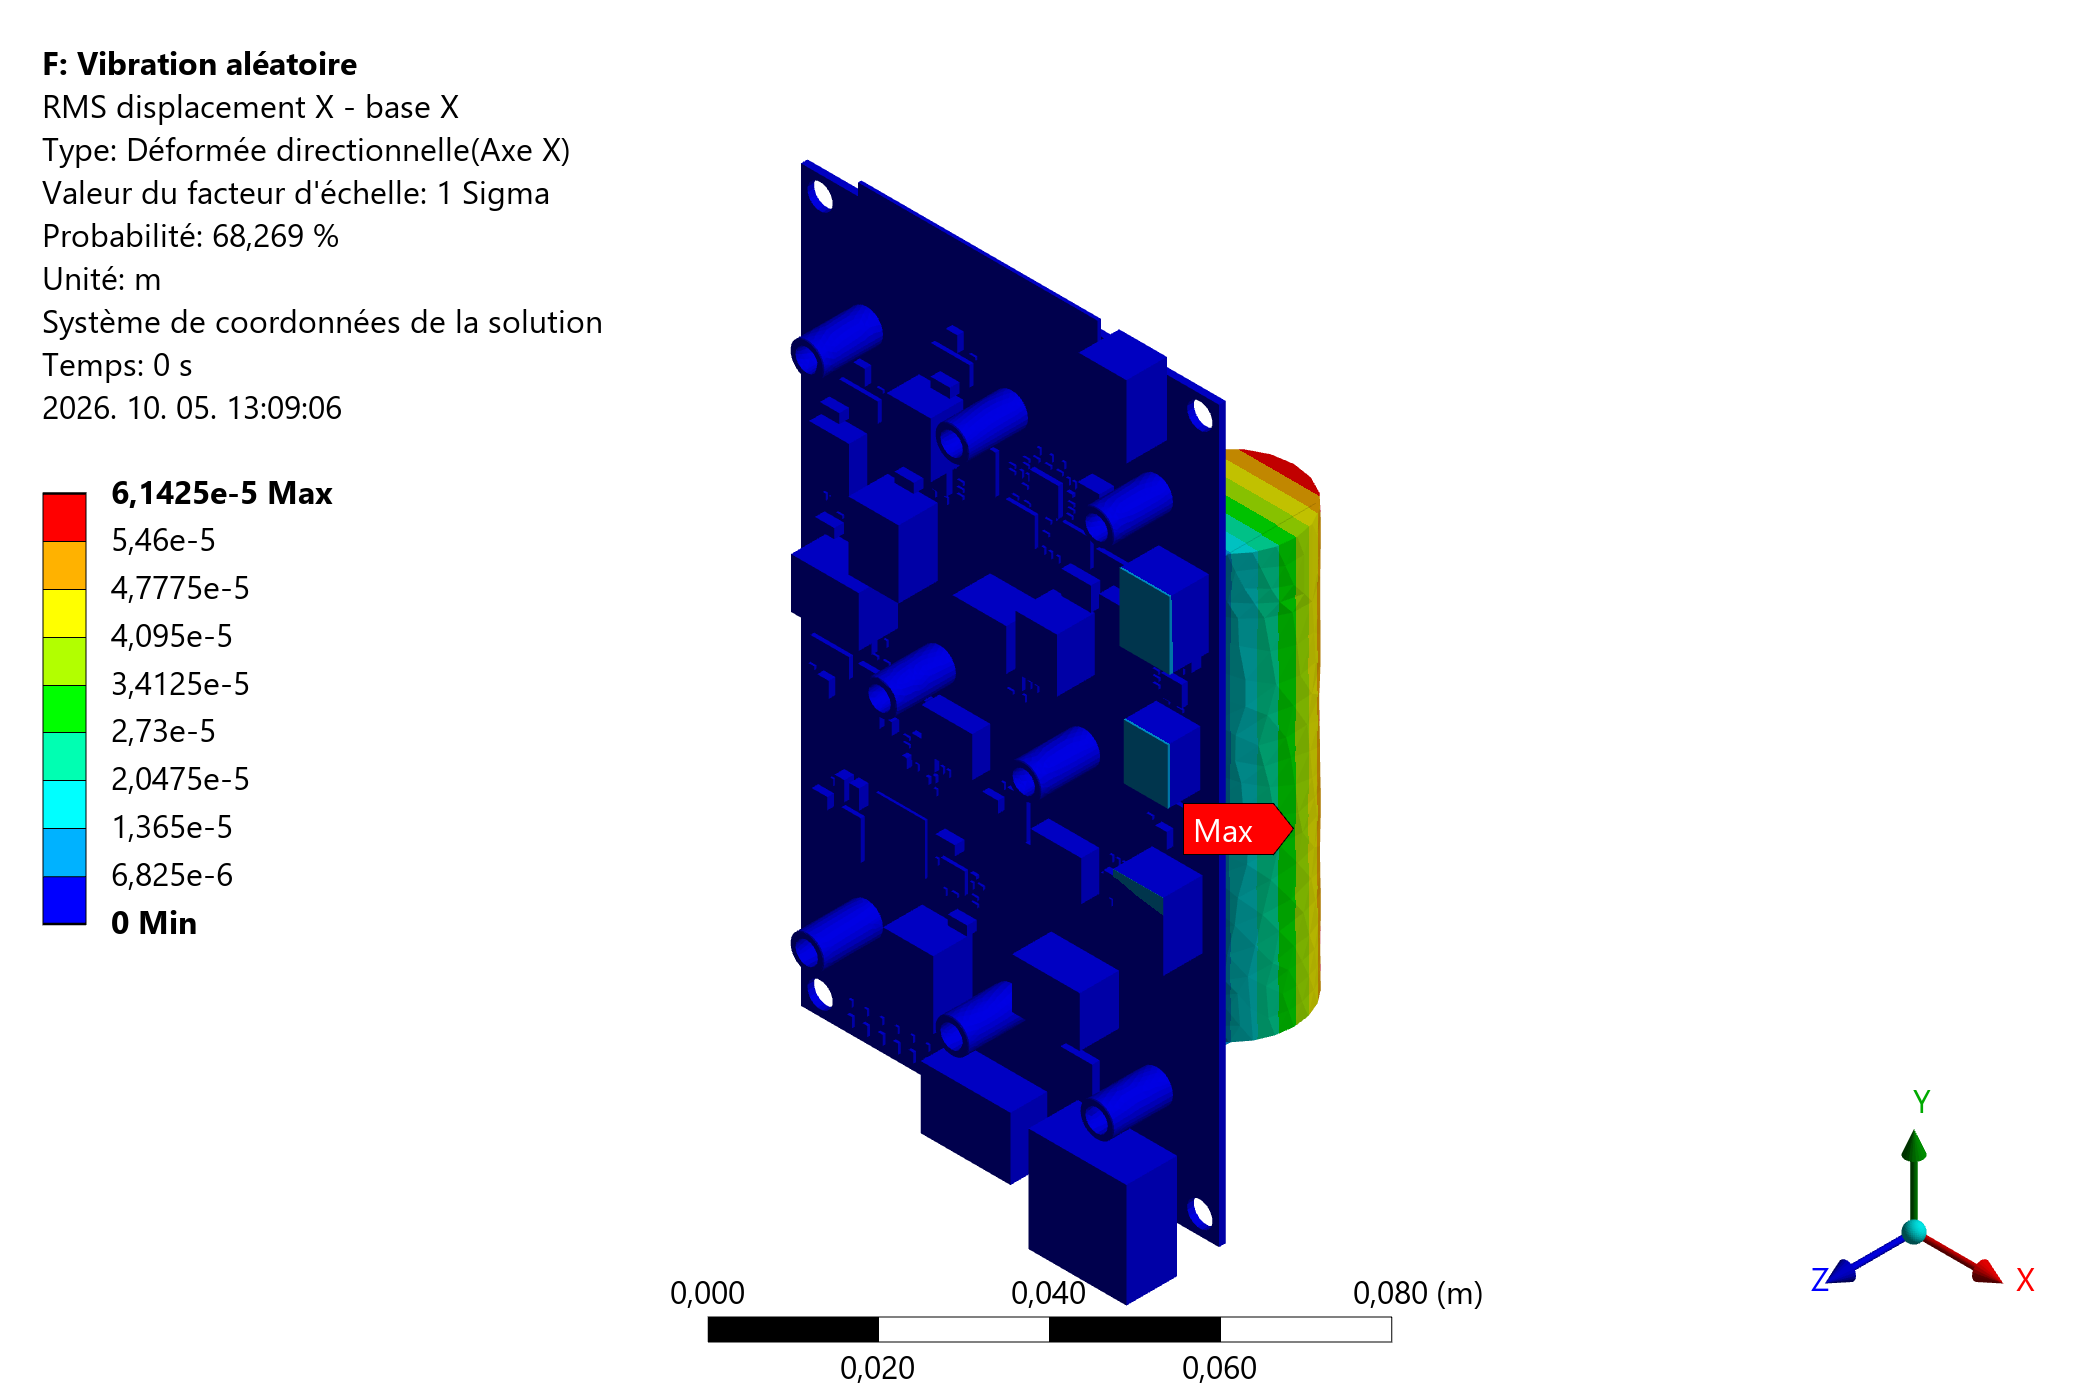
\includegraphics[width=.72\linewidth]{figures/AssemblyX}
\captionof{figure}{X-axis base excitation, whole assembly: X-direction RMS displacement. Spatial maximum 0.061425 mm. PCB, component bodies, batteries and hardware are included. Legend units are metres.}
\end{center}
\begin{center}
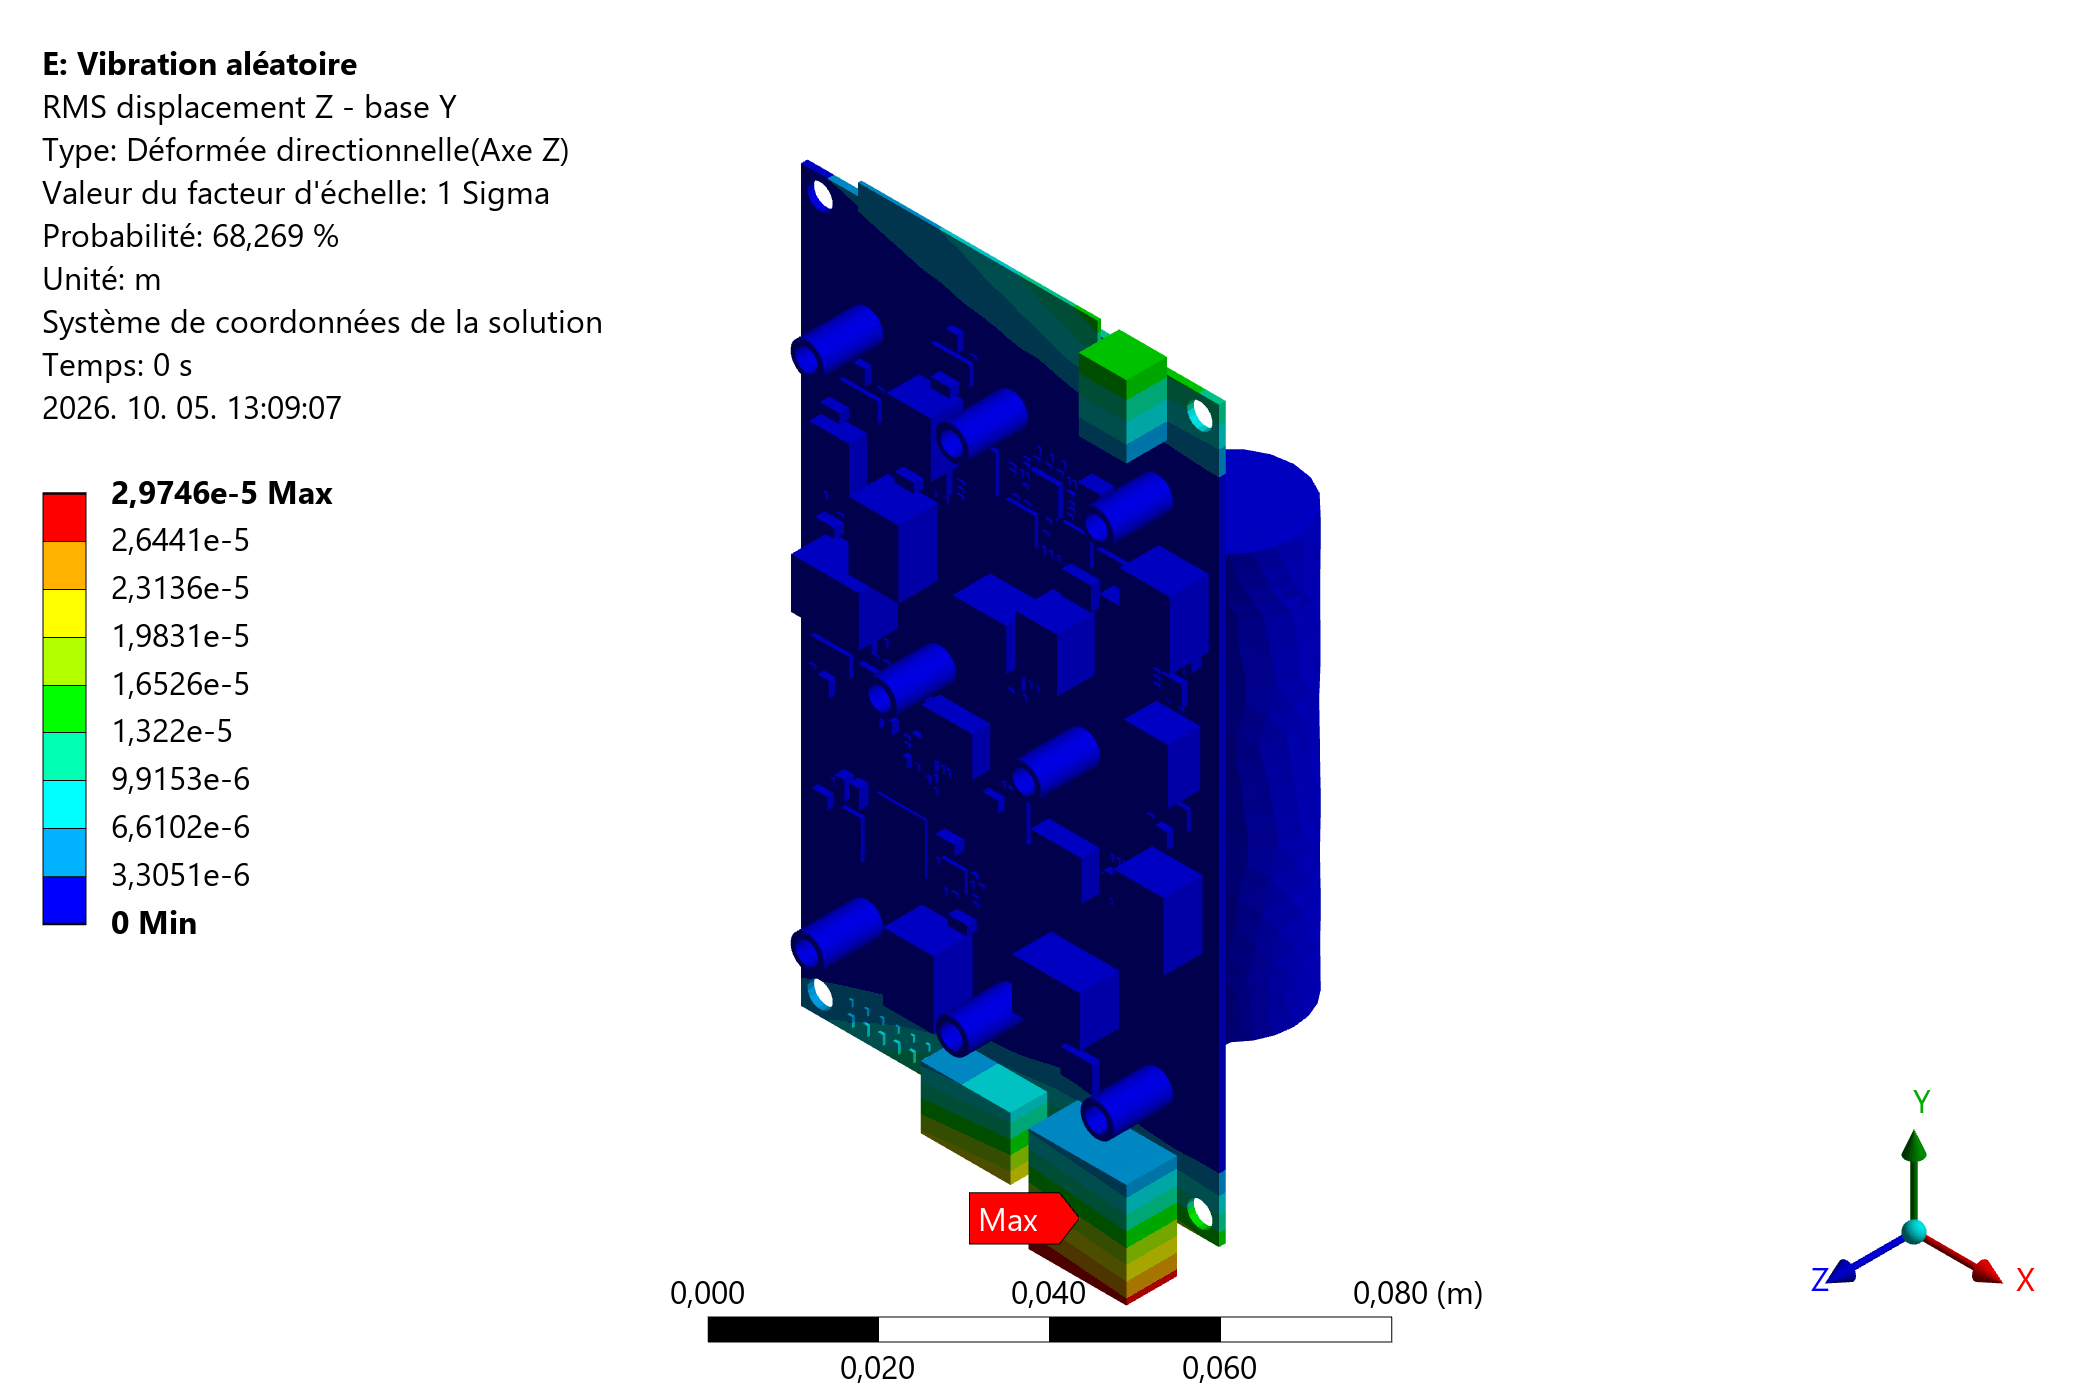
\includegraphics[width=.72\linewidth]{figures/AssemblyY}
\captionof{figure}{Y-axis base excitation, whole assembly: Z-direction RMS displacement. Spatial maximum 0.029746 mm. PCB, component bodies, batteries and hardware are included. Legend units are metres.}
\end{center}
\clearpage\PageTitle{Whole-assembly response: Z excitation and battery side}
\begin{center}
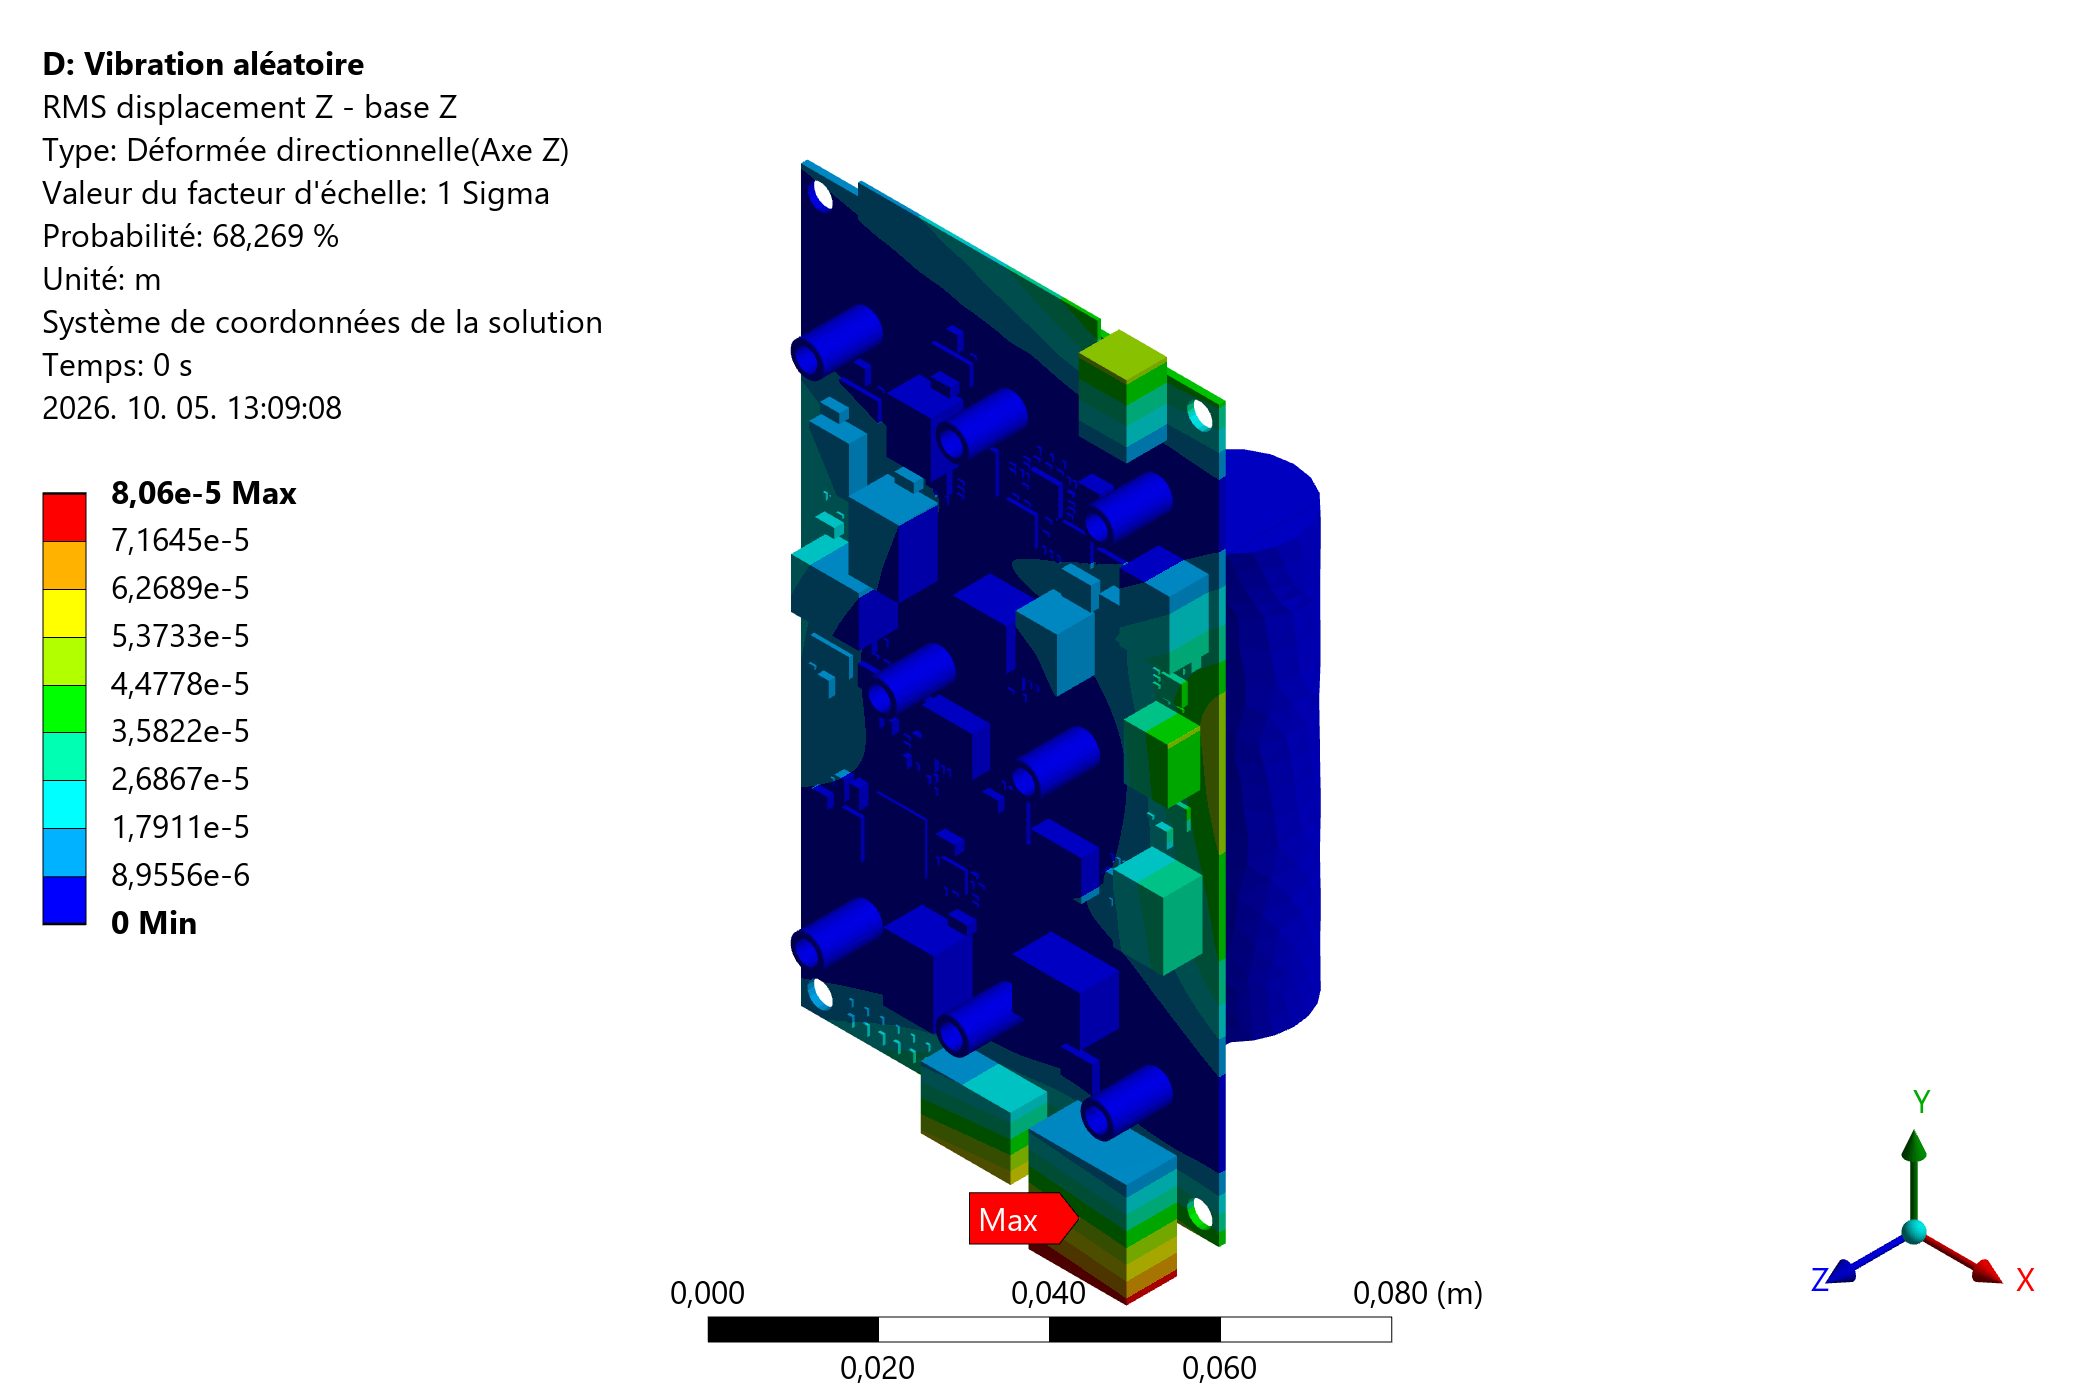
\includegraphics[width=.72\linewidth]{figures/AssemblyZ}
\captionof{figure}{Z-axis base excitation, whole assembly: Z-direction RMS displacement, maximum 0.080600 mm. The populated component side and fastening hardware are visible.}
\end{center}
\begin{center}
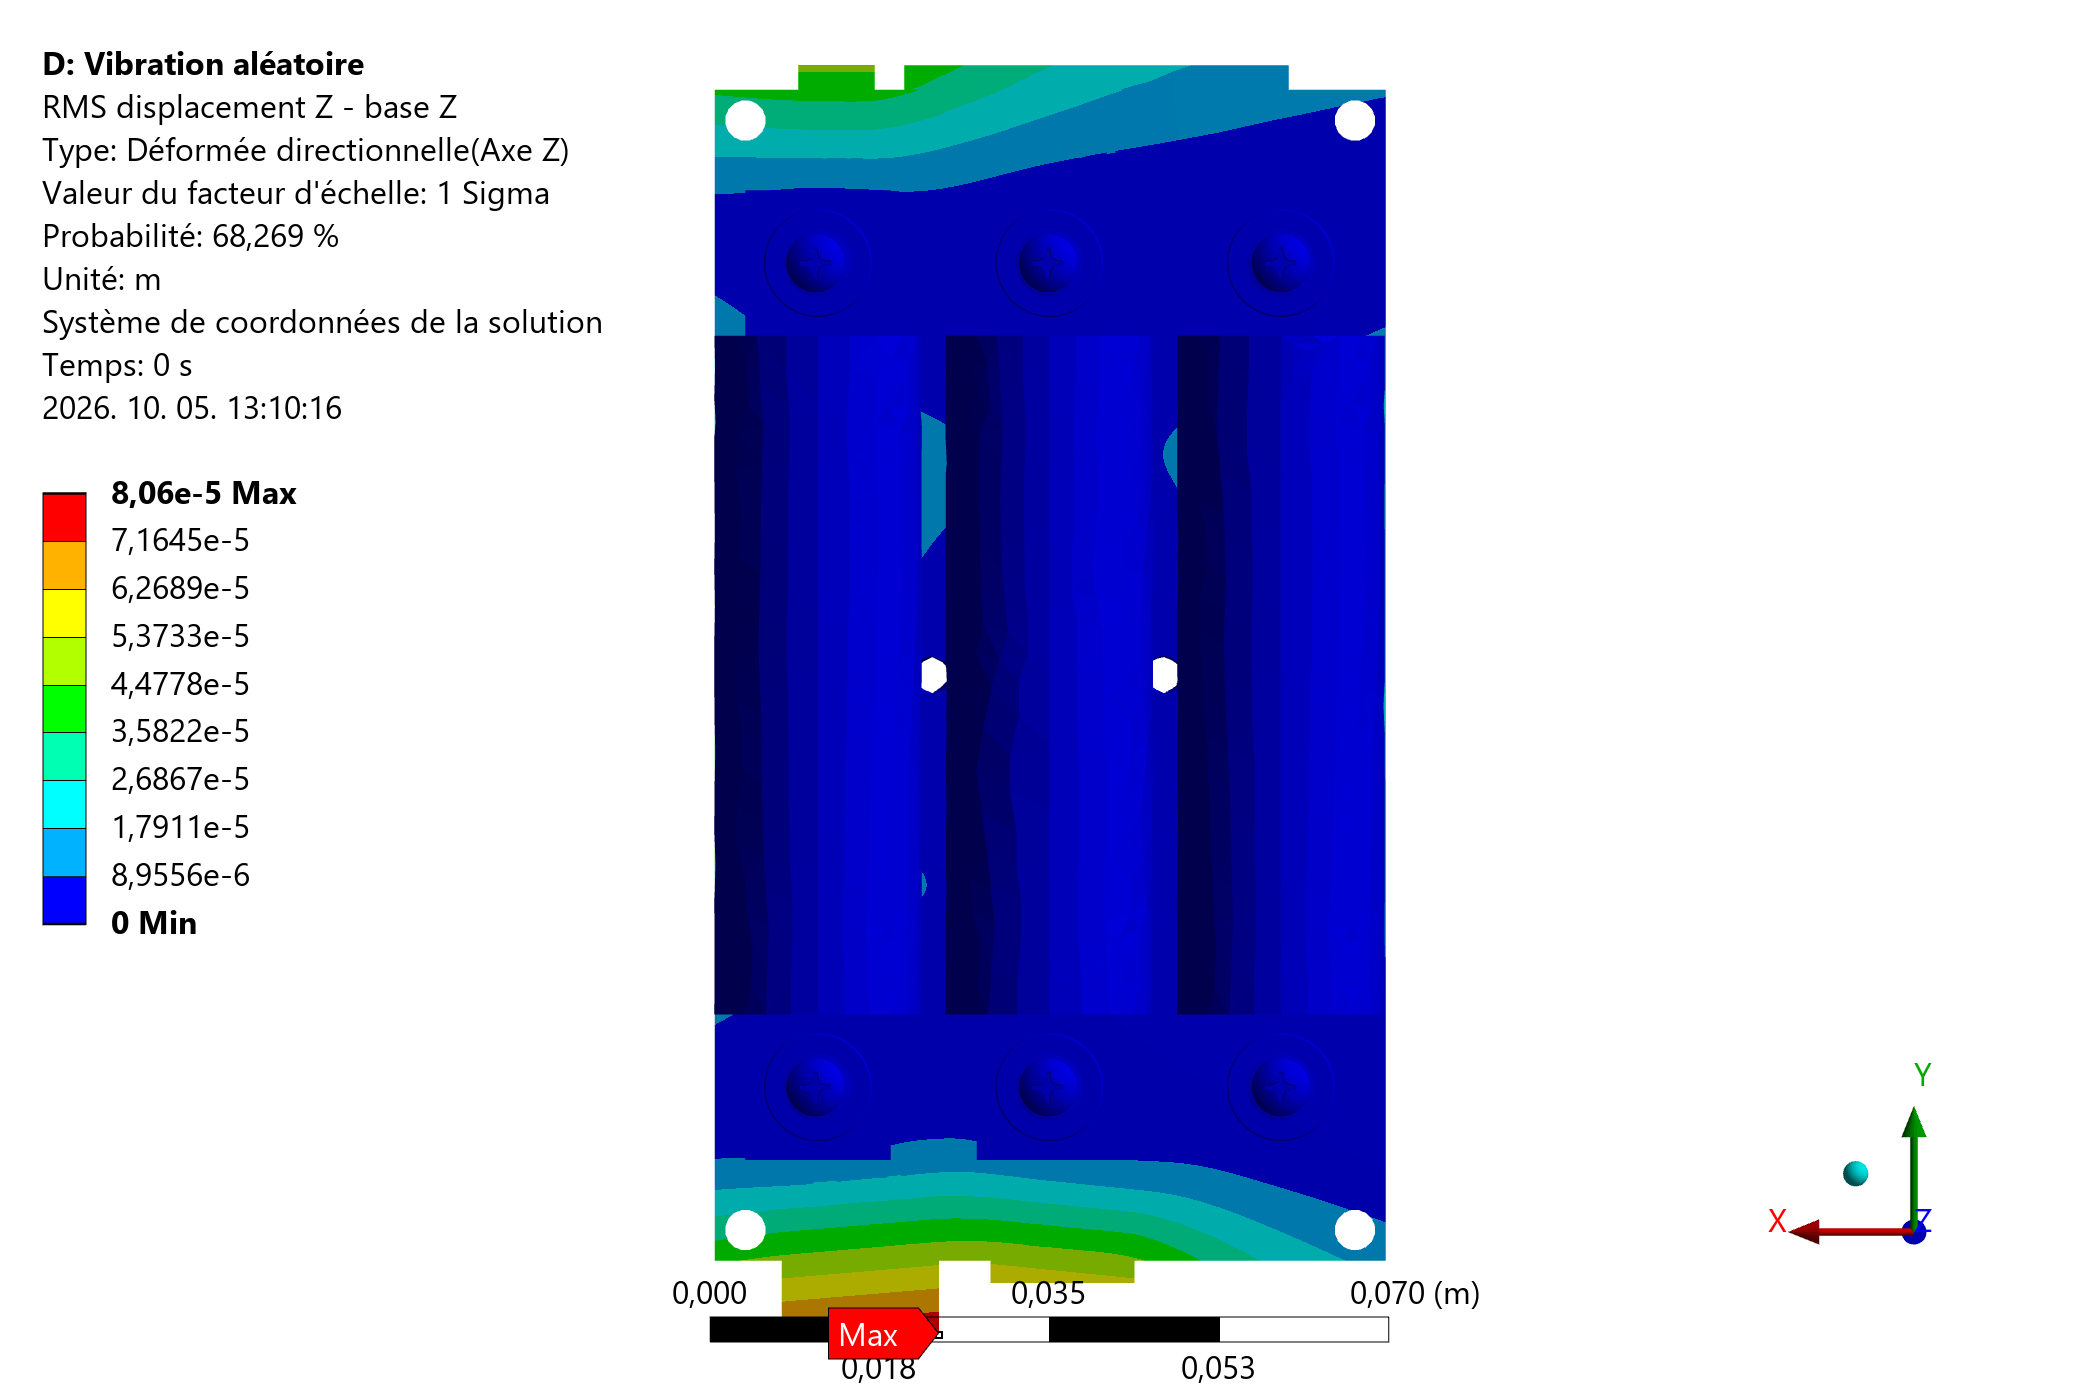
\includegraphics[width=.72\linewidth]{figures/AssemblyBack}
\captionof{figure}{Battery-side view of the same Z-excitation result. The three cell bodies and the six battery fasteners are visible. All figures show the full assembly result; hidden surfaces are occluded by the viewing direction.}
\end{center}
These are directional RMS response contours, not instantaneous vibration shapes. Each contour uses its own range. Imported ECAD components are represented by their meshed solids; this does not establish detailed package or solder-joint accuracy.

\clearpage\PageTitle{Battery-side directional responses}
Fresh native ANSYS views in the requested oblique orientation. All populated assembly bodies remain in the solved model. Each caption distinguishes the base-excitation axis from the displacement response component.
\begin{center}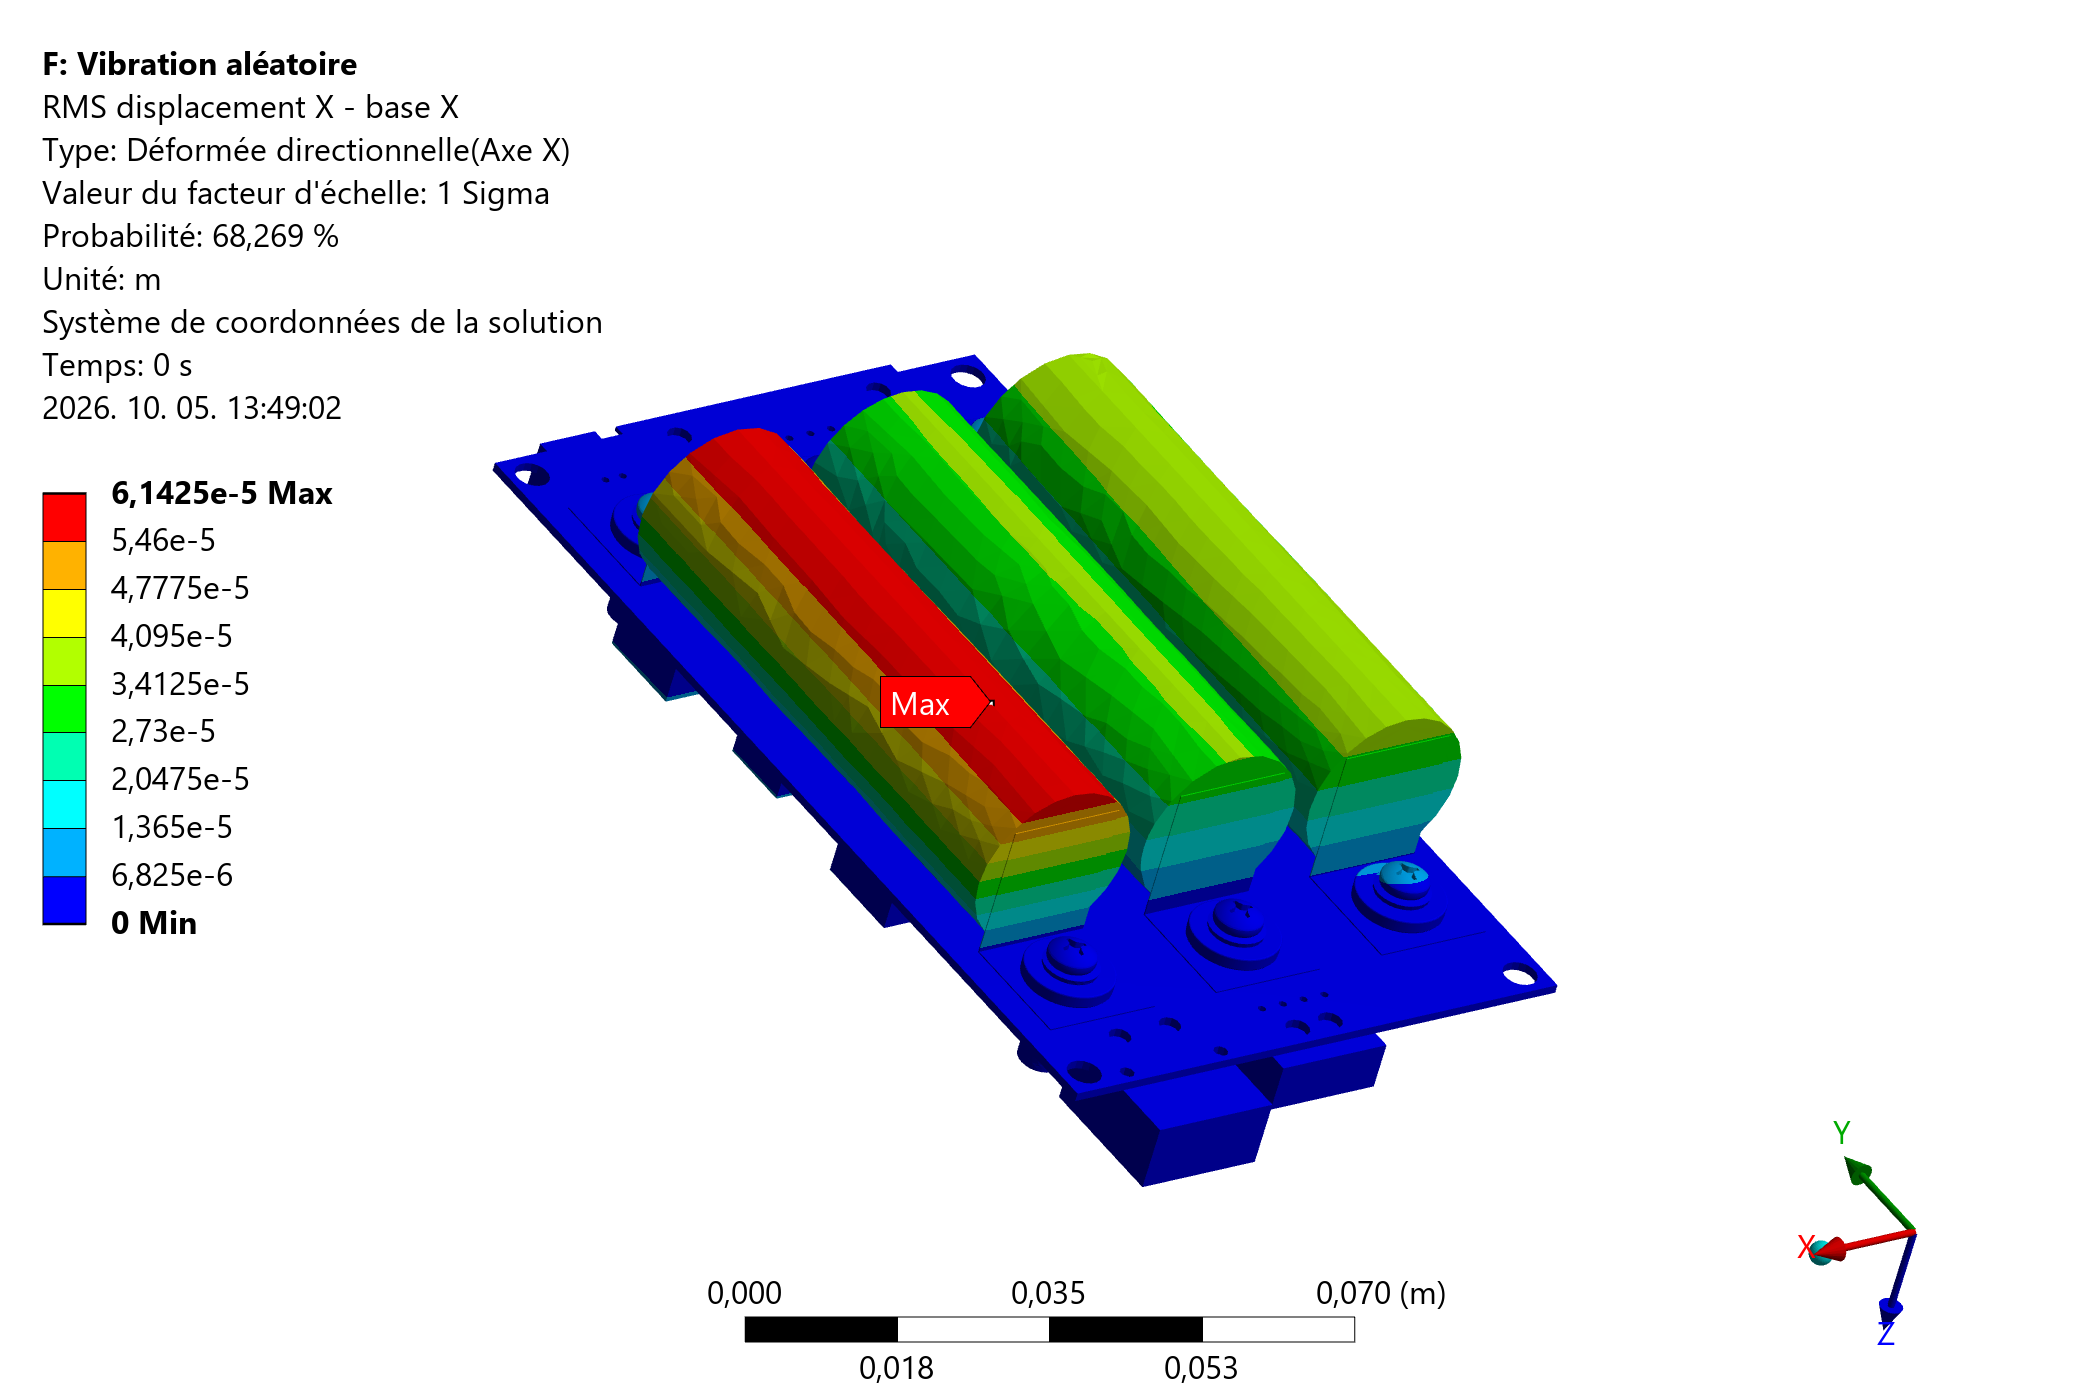
\includegraphics[width=.78\linewidth]{figures/BatteryBaseXResponseX.png}
\captionof{figure}{Base X excitation, global X-direction displacement RMS over the whole assembly. Maximum 0.06142534 mm. One-sigma response; native legend in metres.}\end{center}
\begin{center}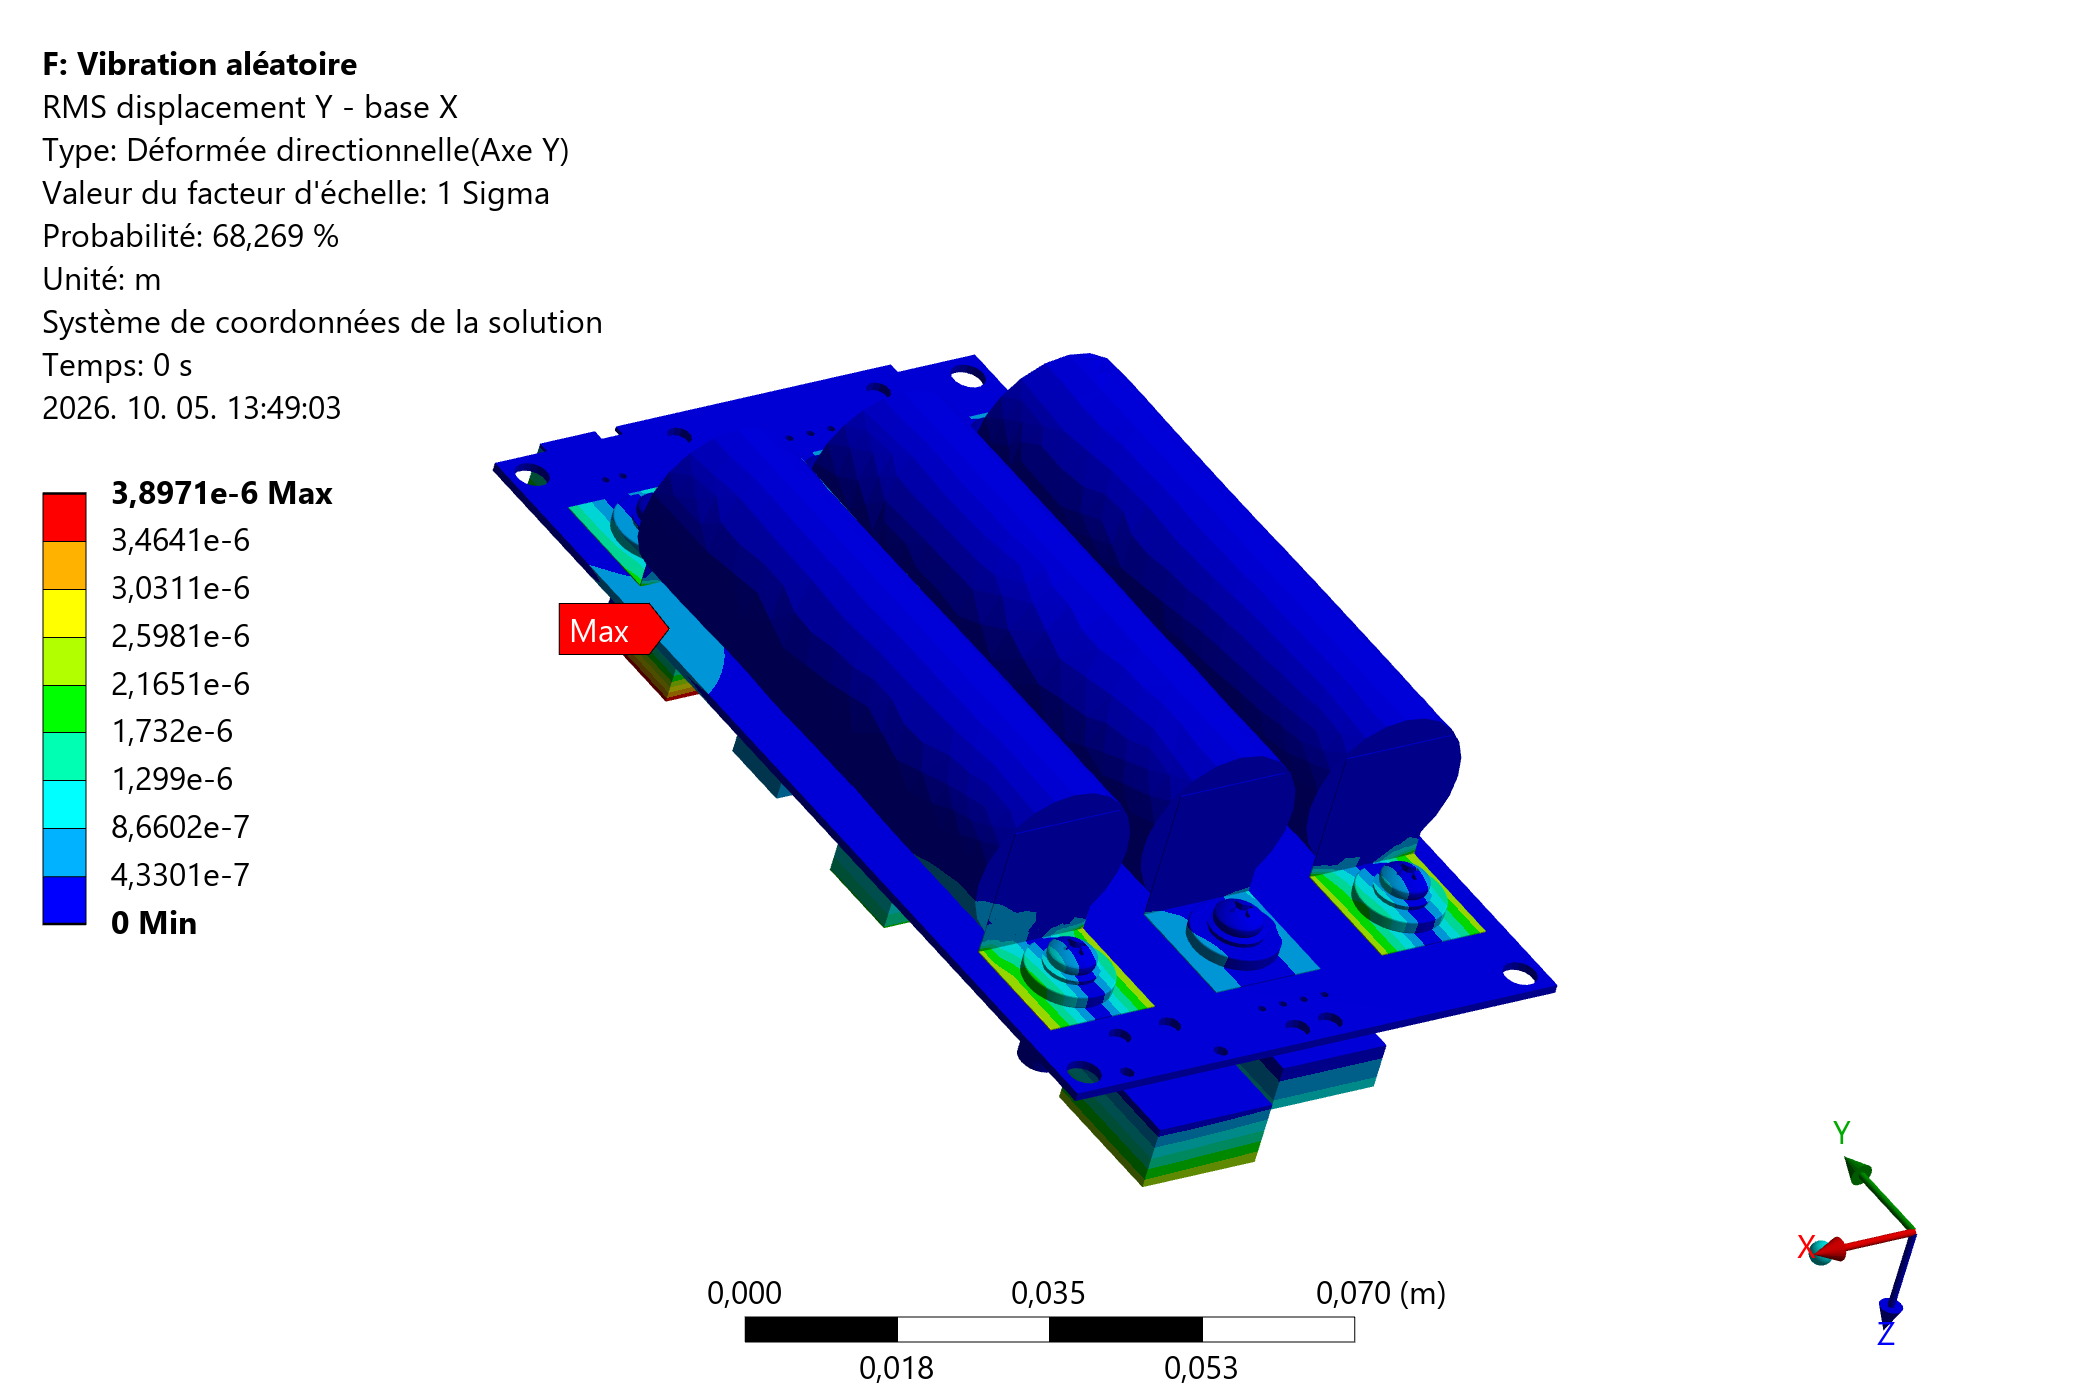
\includegraphics[width=.78\linewidth]{figures/BatteryBaseXResponseY.png}
\captionof{figure}{Base X excitation, global Y-direction displacement RMS over the whole assembly. Maximum 0.003897111 mm. One-sigma response; native legend in metres.}\end{center}
\clearpage\PageTitle{Battery-side directional responses}
\begin{center}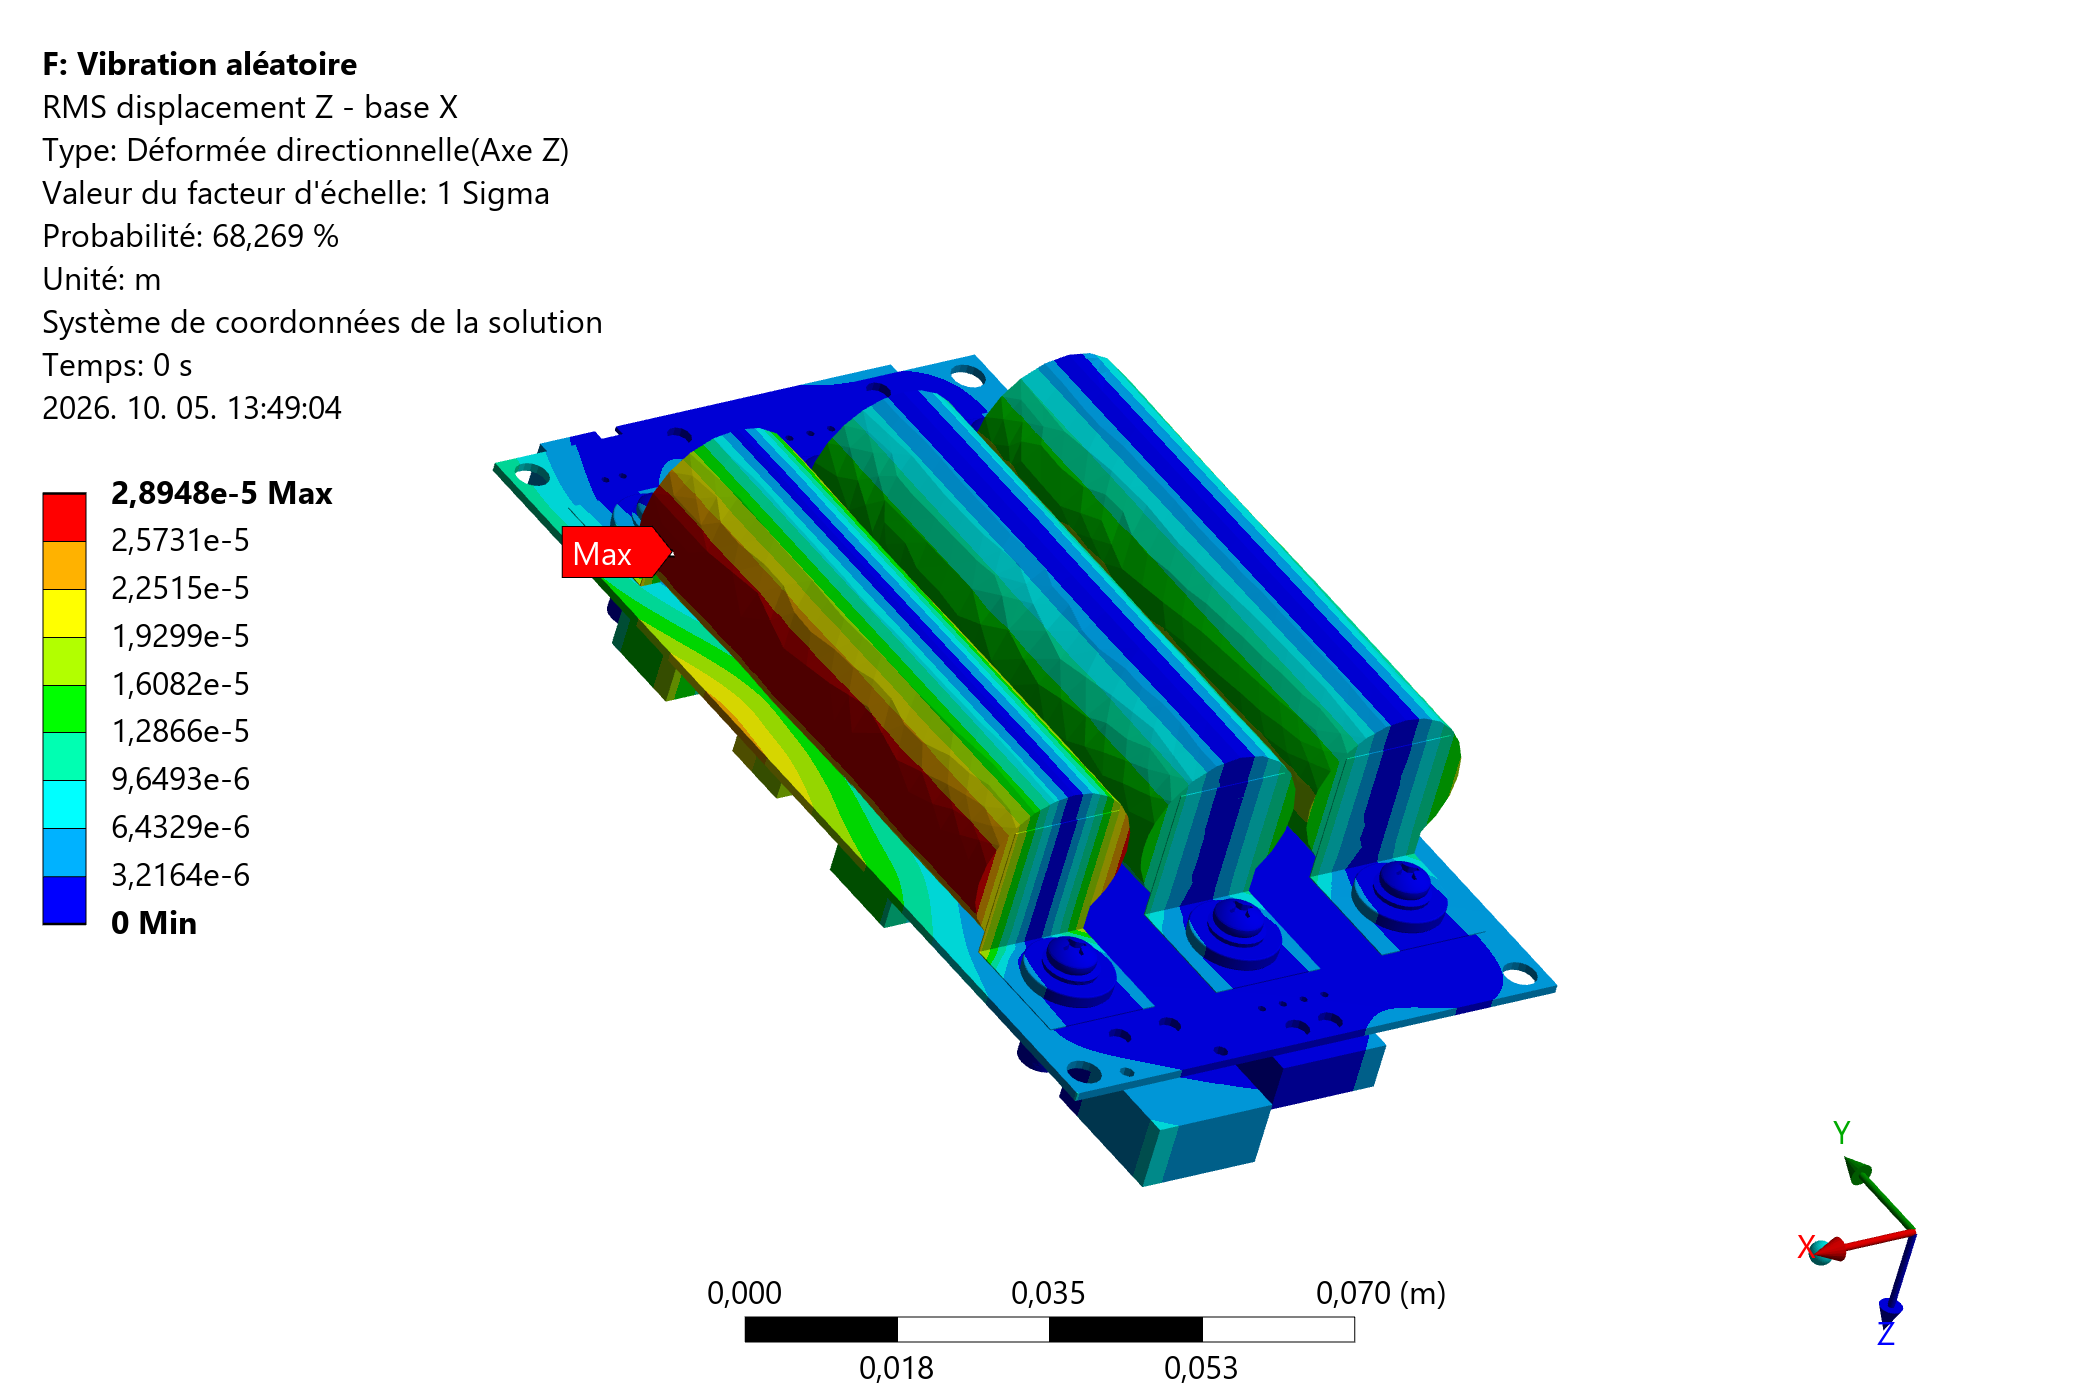
\includegraphics[width=.78\linewidth]{figures/BatteryBaseXResponseZ.png}
\captionof{figure}{Base X excitation, global Z-direction displacement RMS over the whole assembly. Maximum 0.02894789 mm. One-sigma response; native legend in metres.}\end{center}
\begin{center}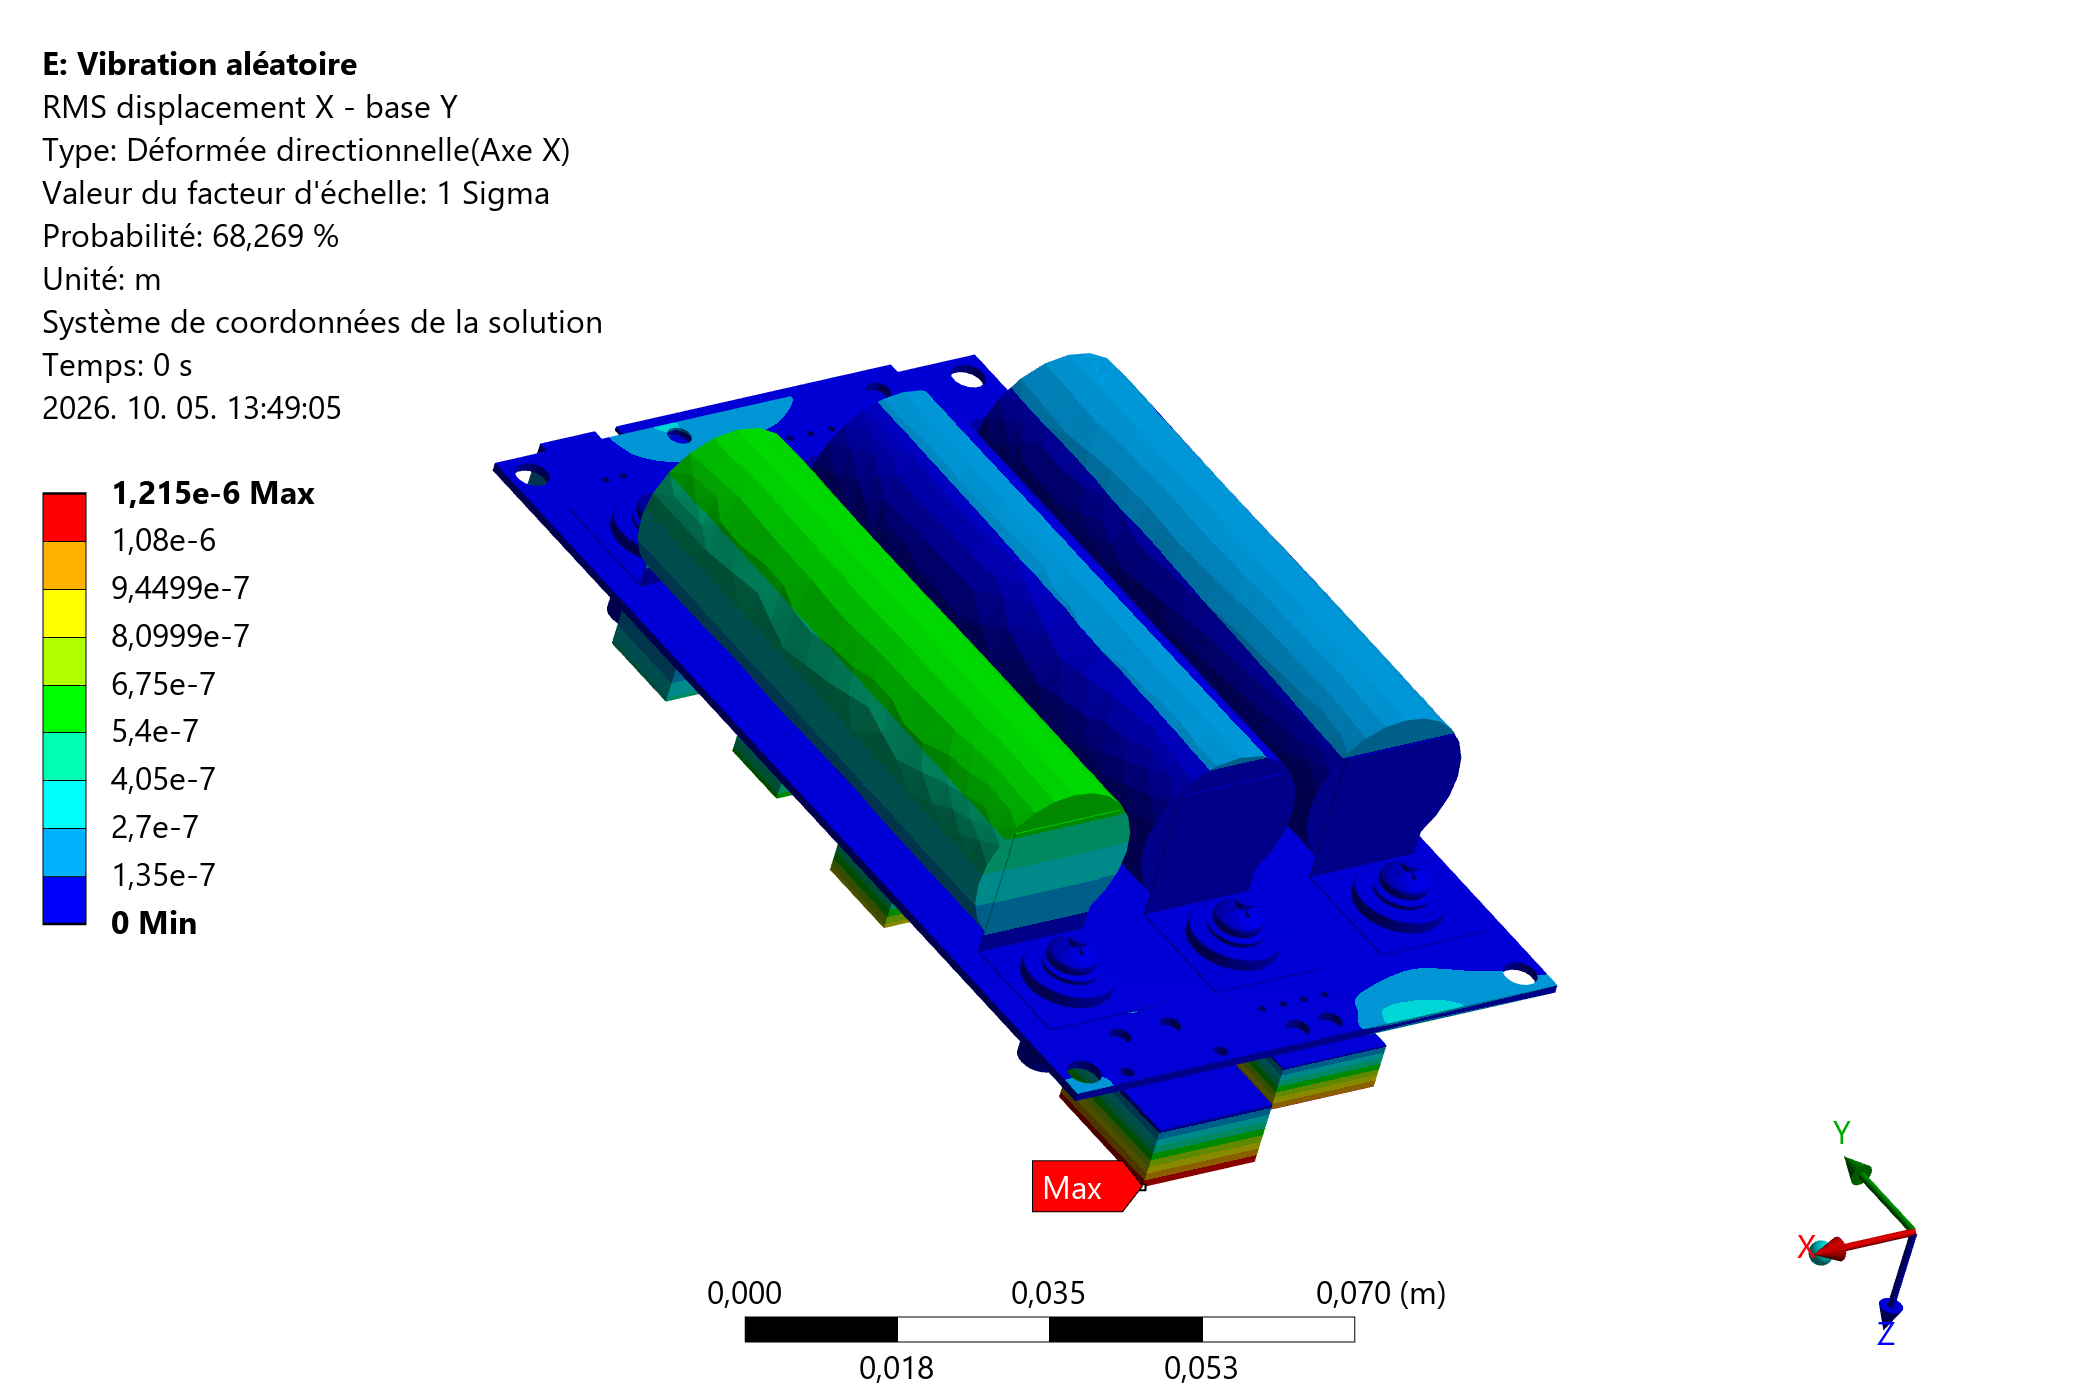
\includegraphics[width=.78\linewidth]{figures/BatteryBaseYResponseX.png}
\captionof{figure}{Base Y excitation, global X-direction displacement RMS over the whole assembly. Maximum 0.001214992 mm. One-sigma response; native legend in metres.}\end{center}
\clearpage\PageTitle{Battery-side directional responses}
\begin{center}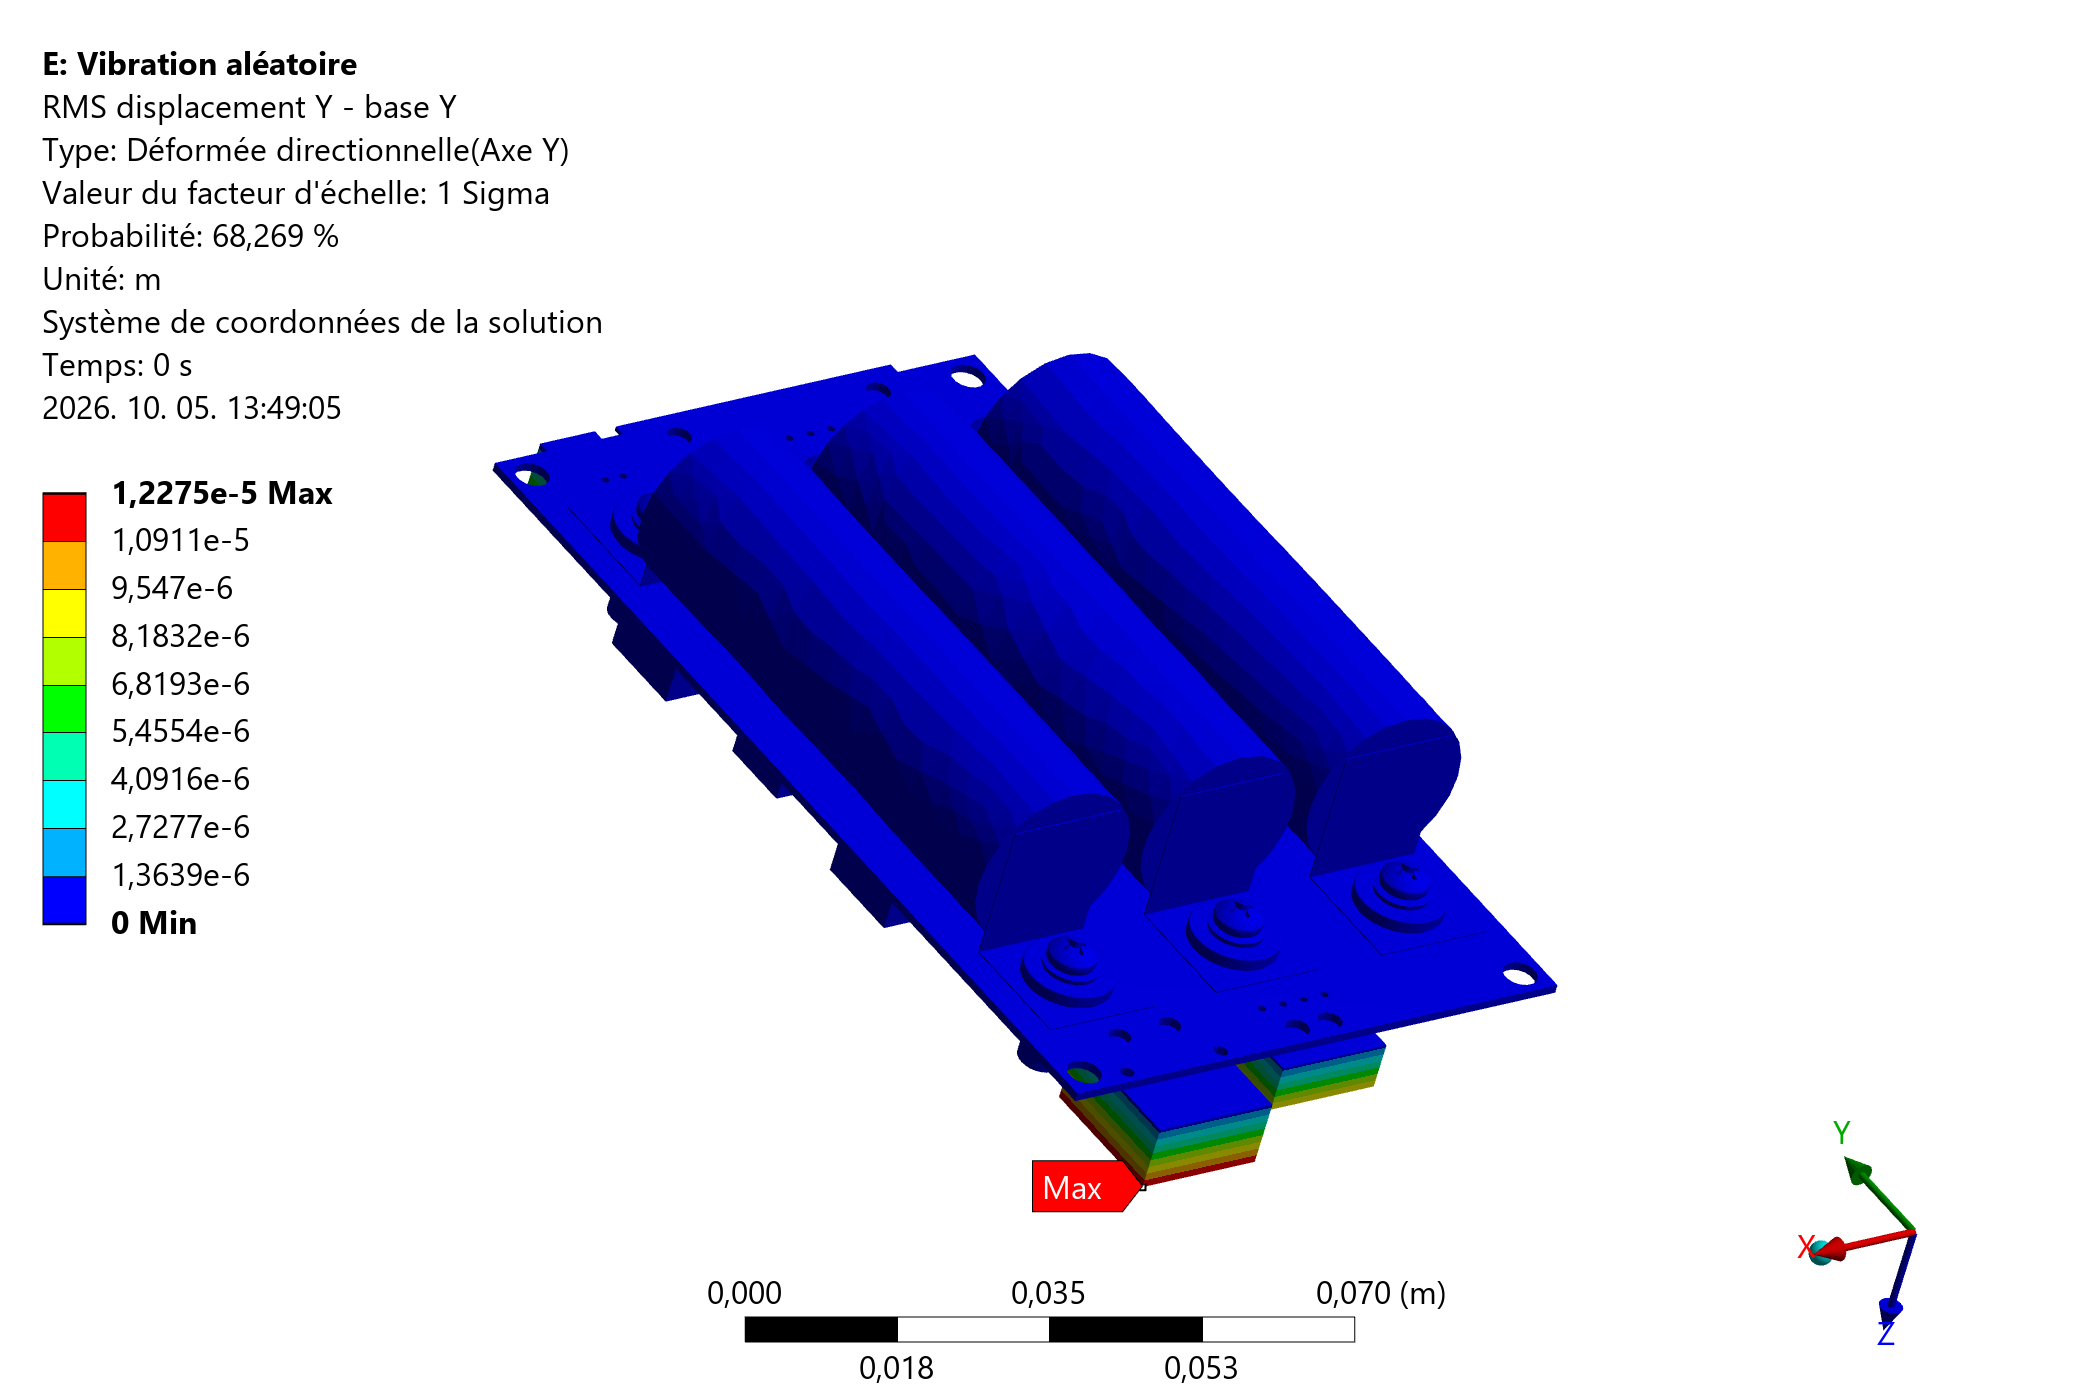
\includegraphics[width=.78\linewidth]{figures/BatteryBaseYResponseY.png}
\captionof{figure}{Base Y excitation, global Y-direction displacement RMS over the whole assembly. Maximum 0.01227474 mm. One-sigma response; native legend in metres.}\end{center}
\begin{center}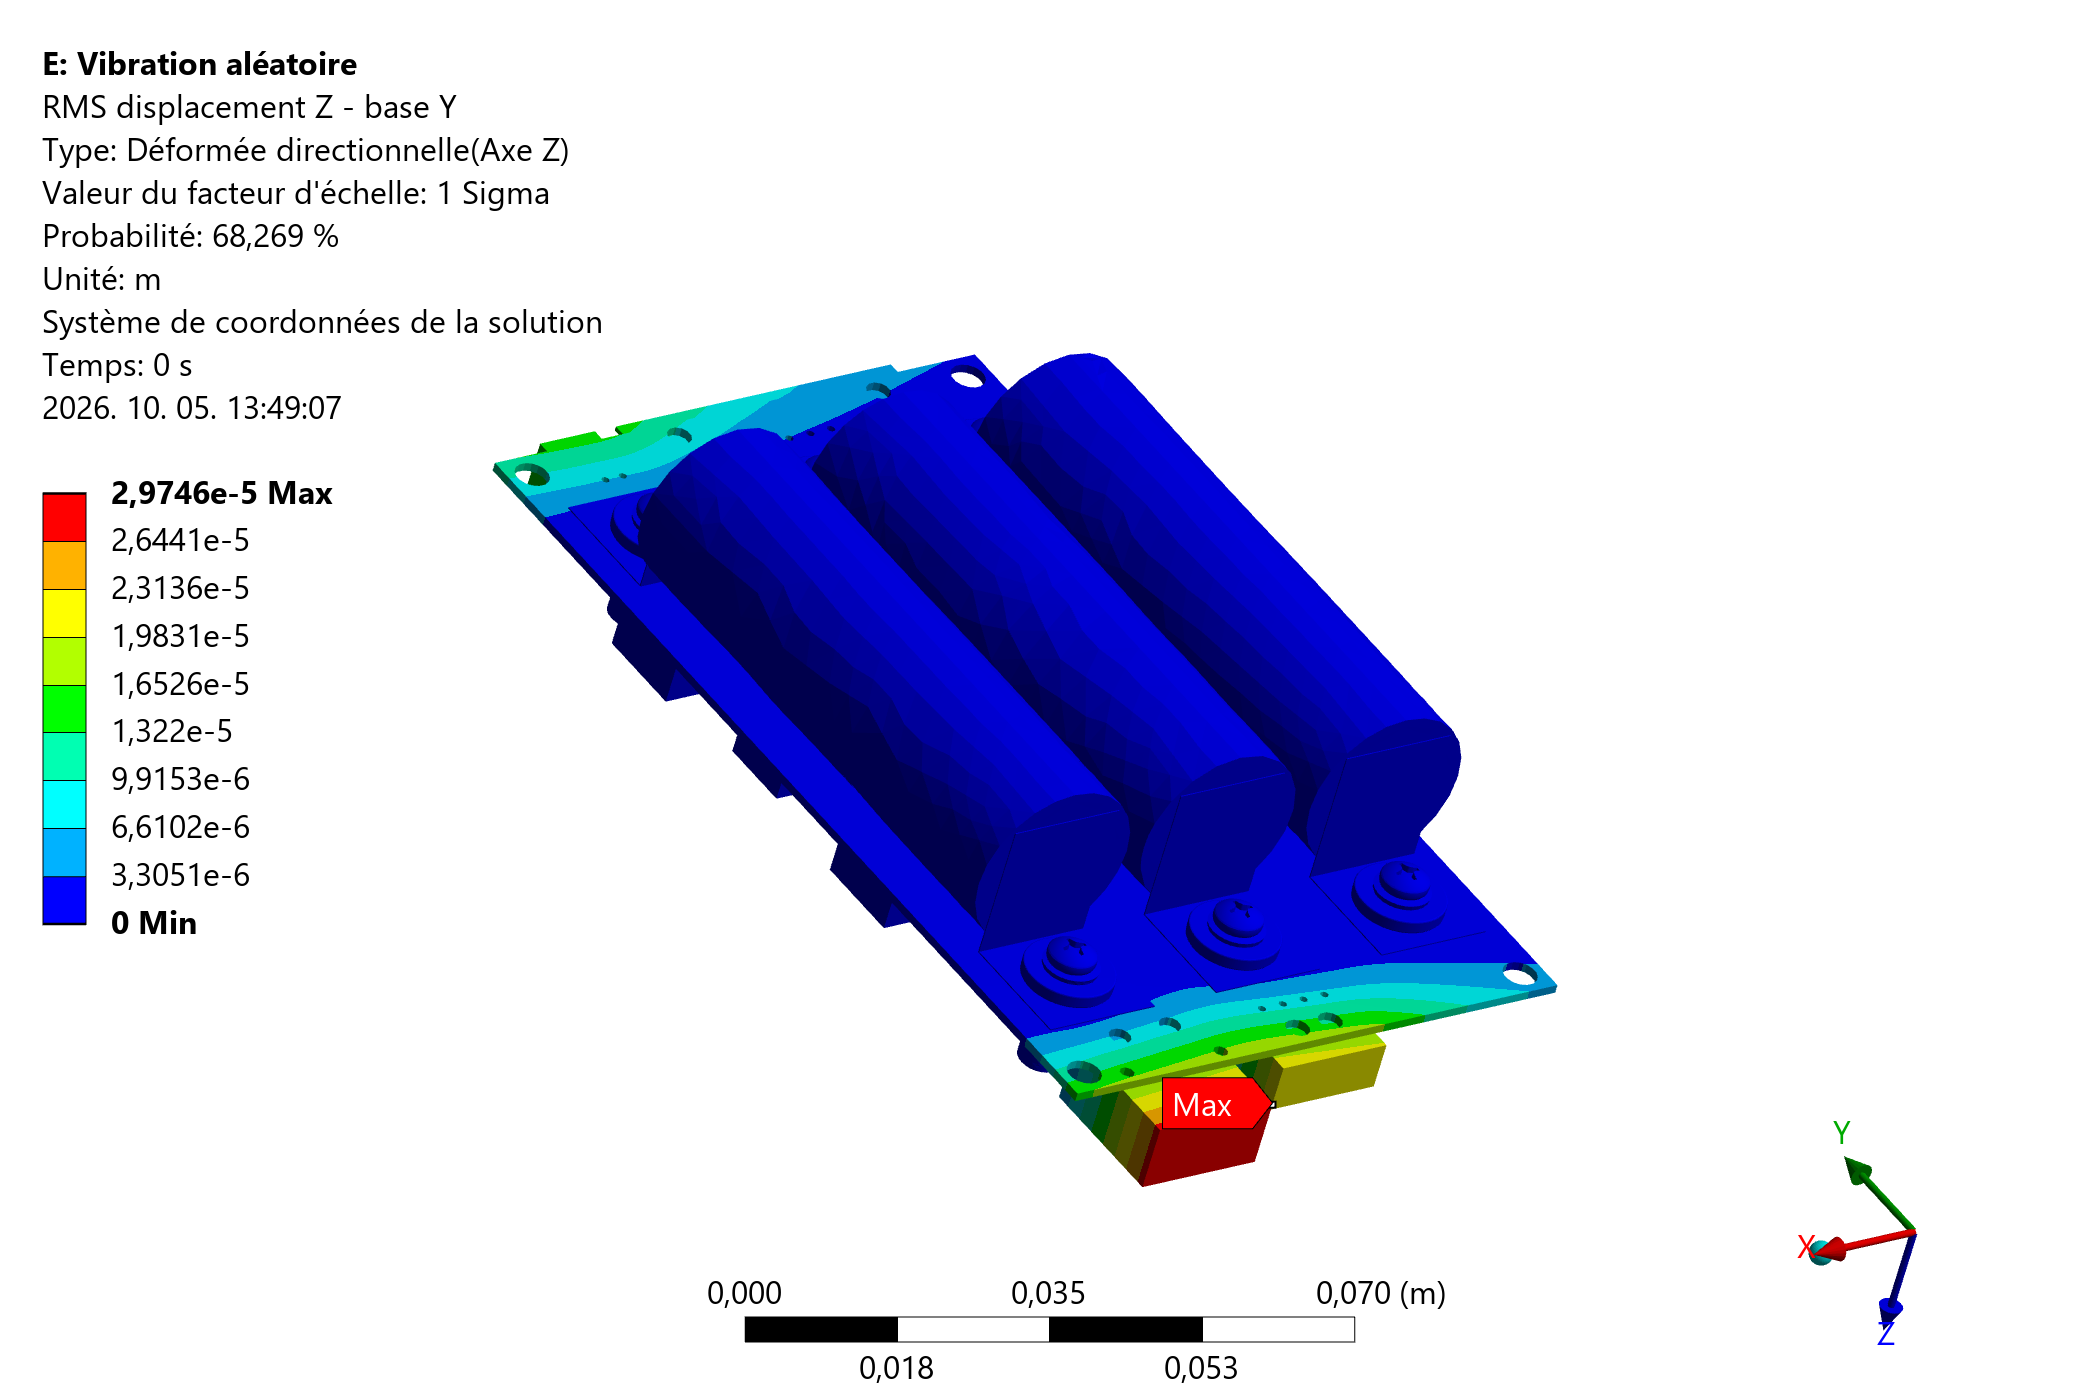
\includegraphics[width=.78\linewidth]{figures/BatteryBaseYResponseZ.png}
\captionof{figure}{Base Y excitation, global Z-direction displacement RMS over the whole assembly. Maximum 0.02974601 mm. One-sigma response; native legend in metres.}\end{center}
\clearpage\PageTitle{Battery-side directional responses}
\begin{center}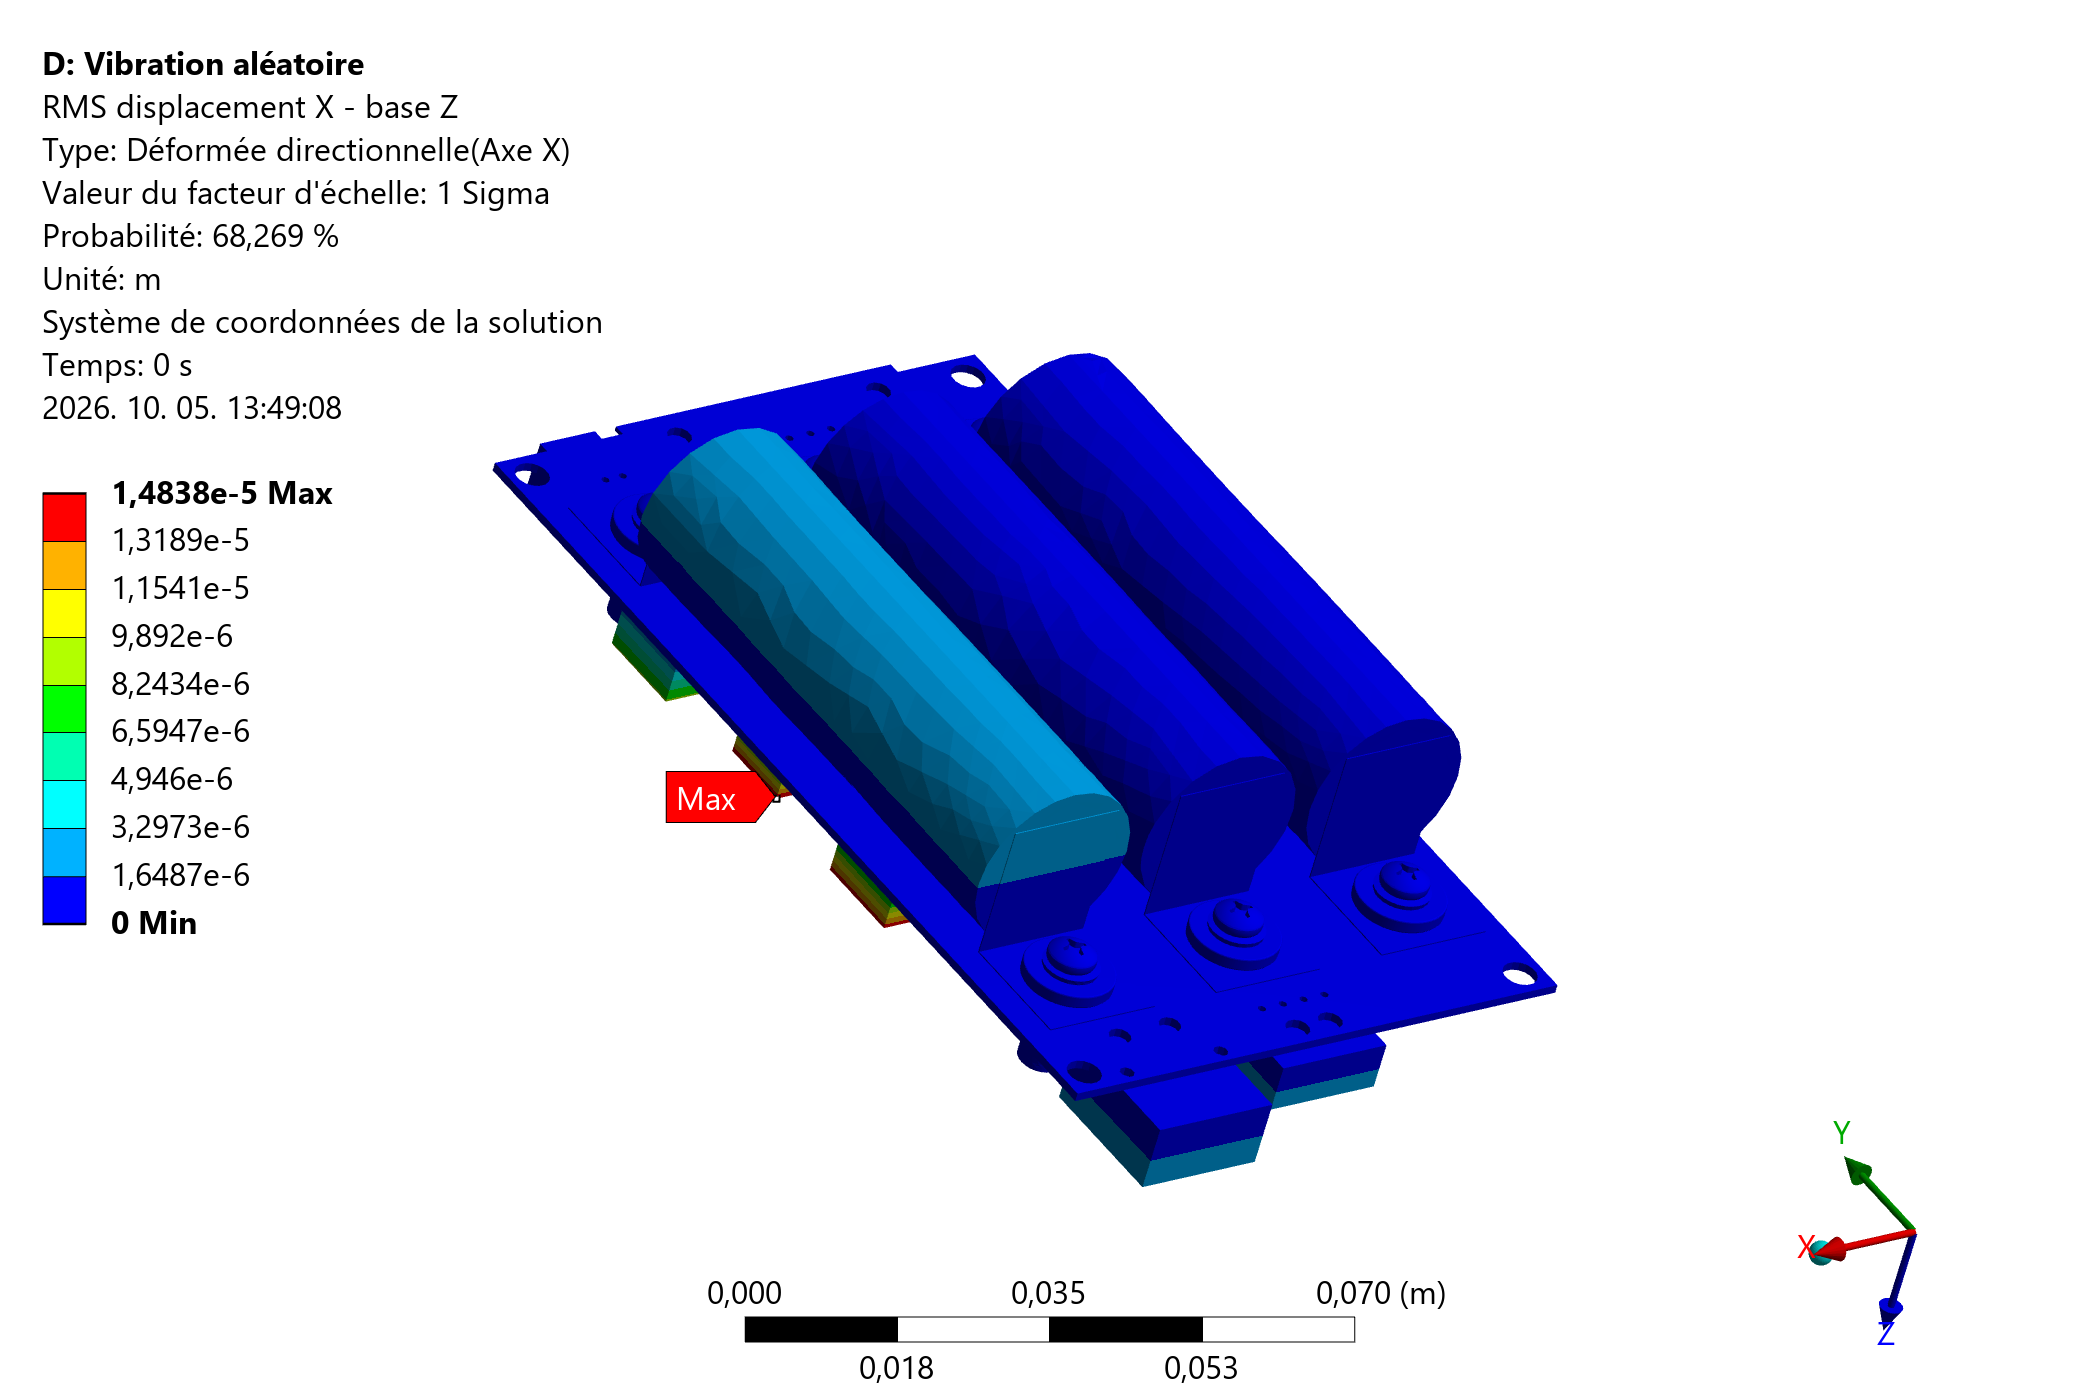
\includegraphics[width=.78\linewidth]{figures/BatteryBaseZResponseX.png}
\captionof{figure}{Base Z excitation, global X-direction displacement RMS over the whole assembly. Maximum 0.01483805 mm. One-sigma response; native legend in metres.}\end{center}
\begin{center}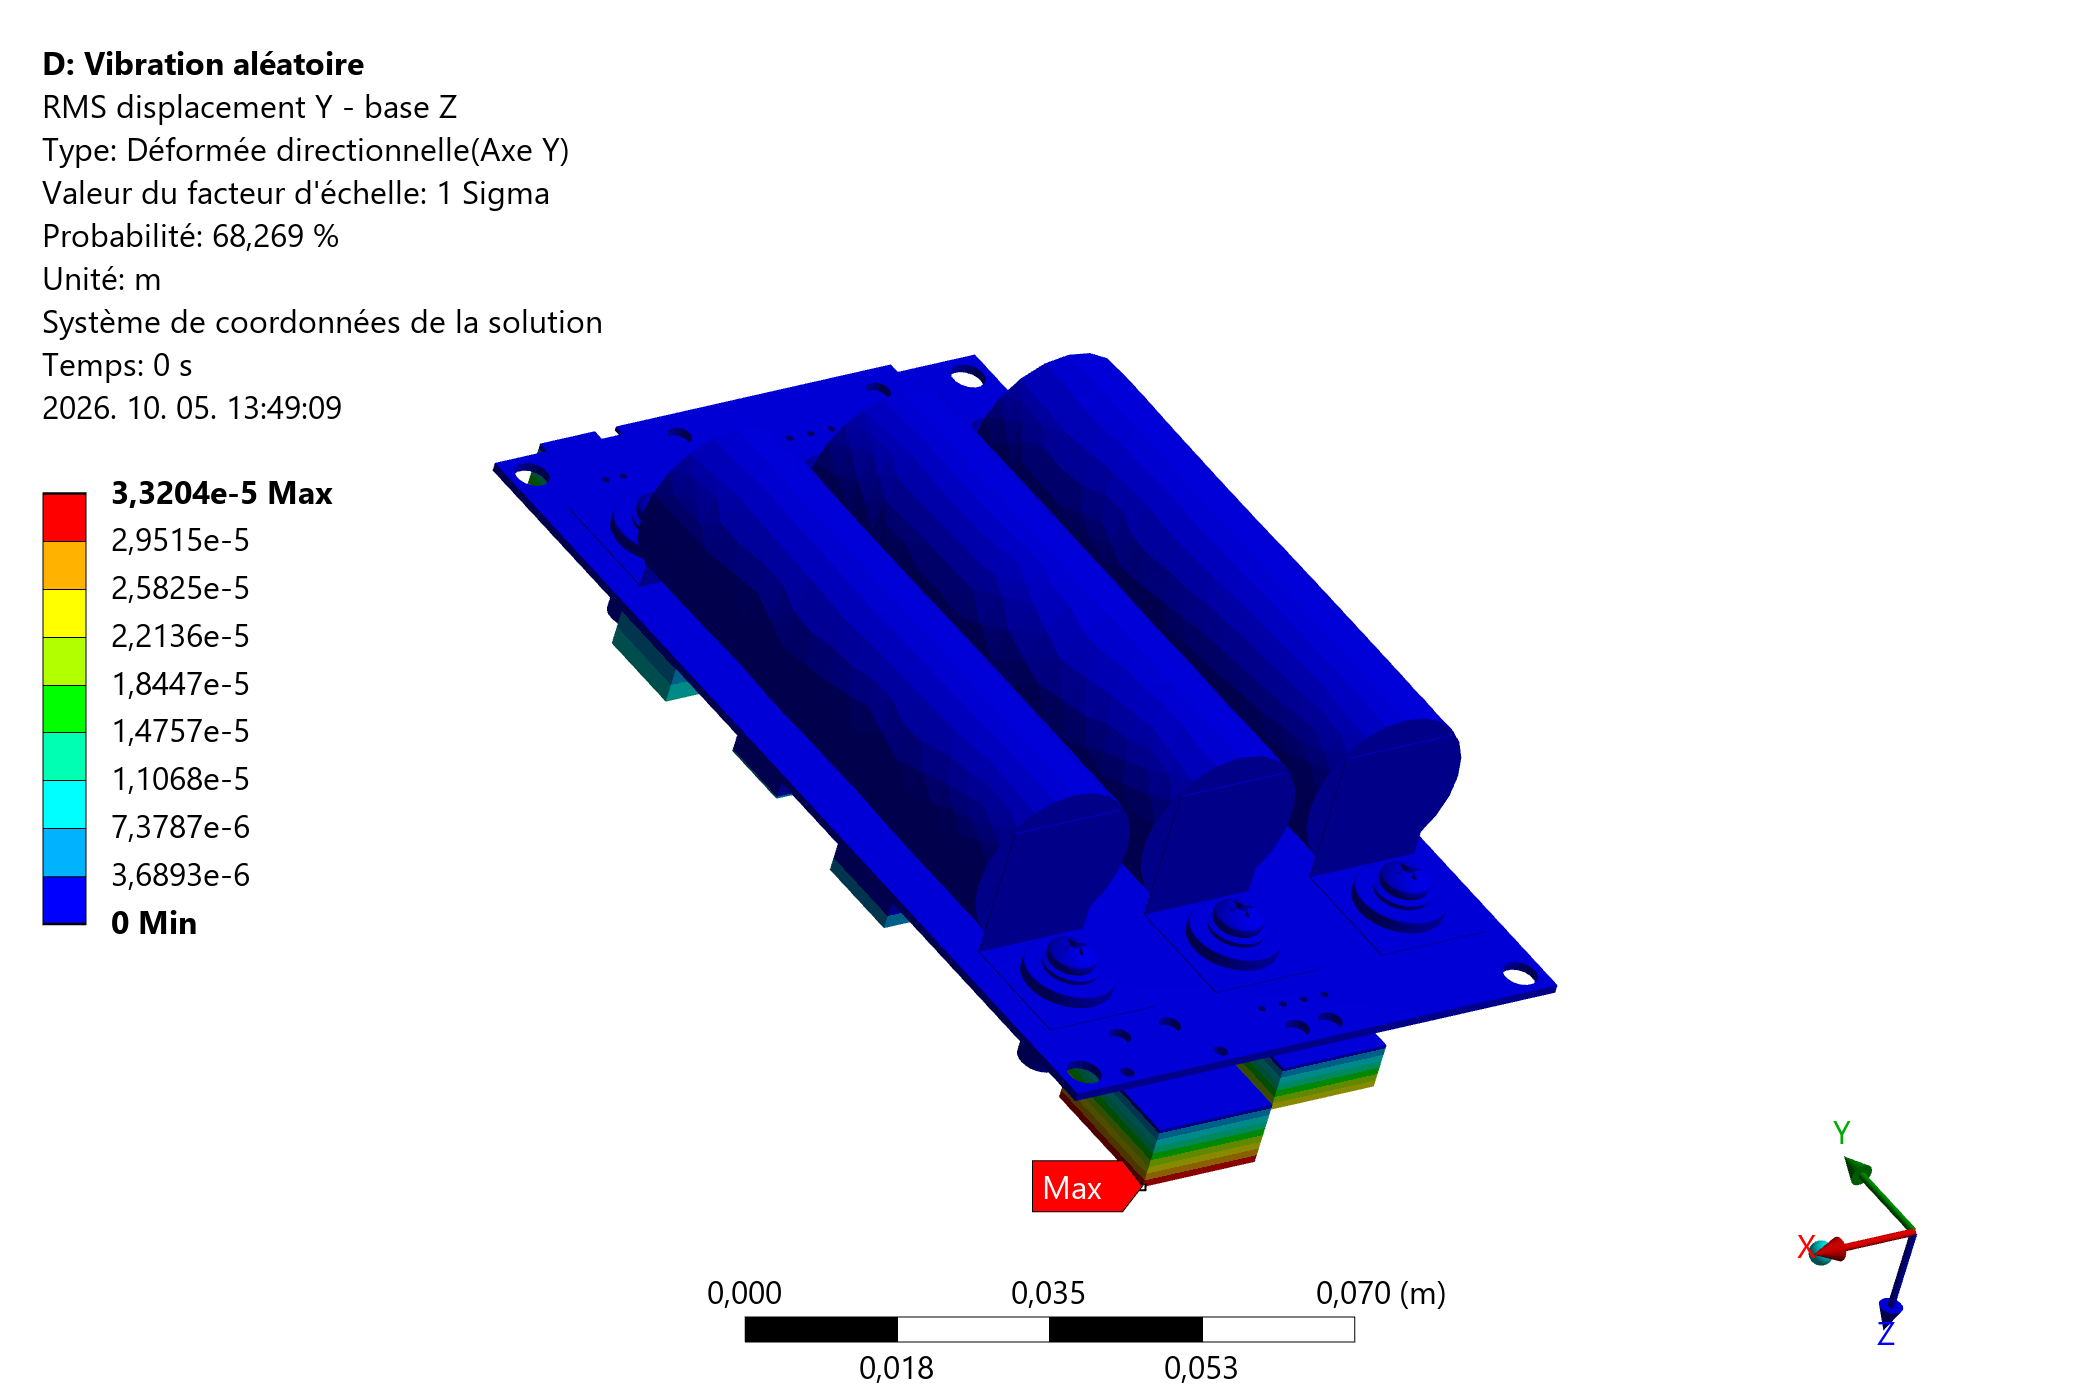
\includegraphics[width=.78\linewidth]{figures/BatteryBaseZResponseY.png}
\captionof{figure}{Base Z excitation, global Y-direction displacement RMS over the whole assembly. Maximum 0.03320397 mm. One-sigma response; native legend in metres.}\end{center}
\clearpage\PageTitle{Battery-side directional response}
\begin{center}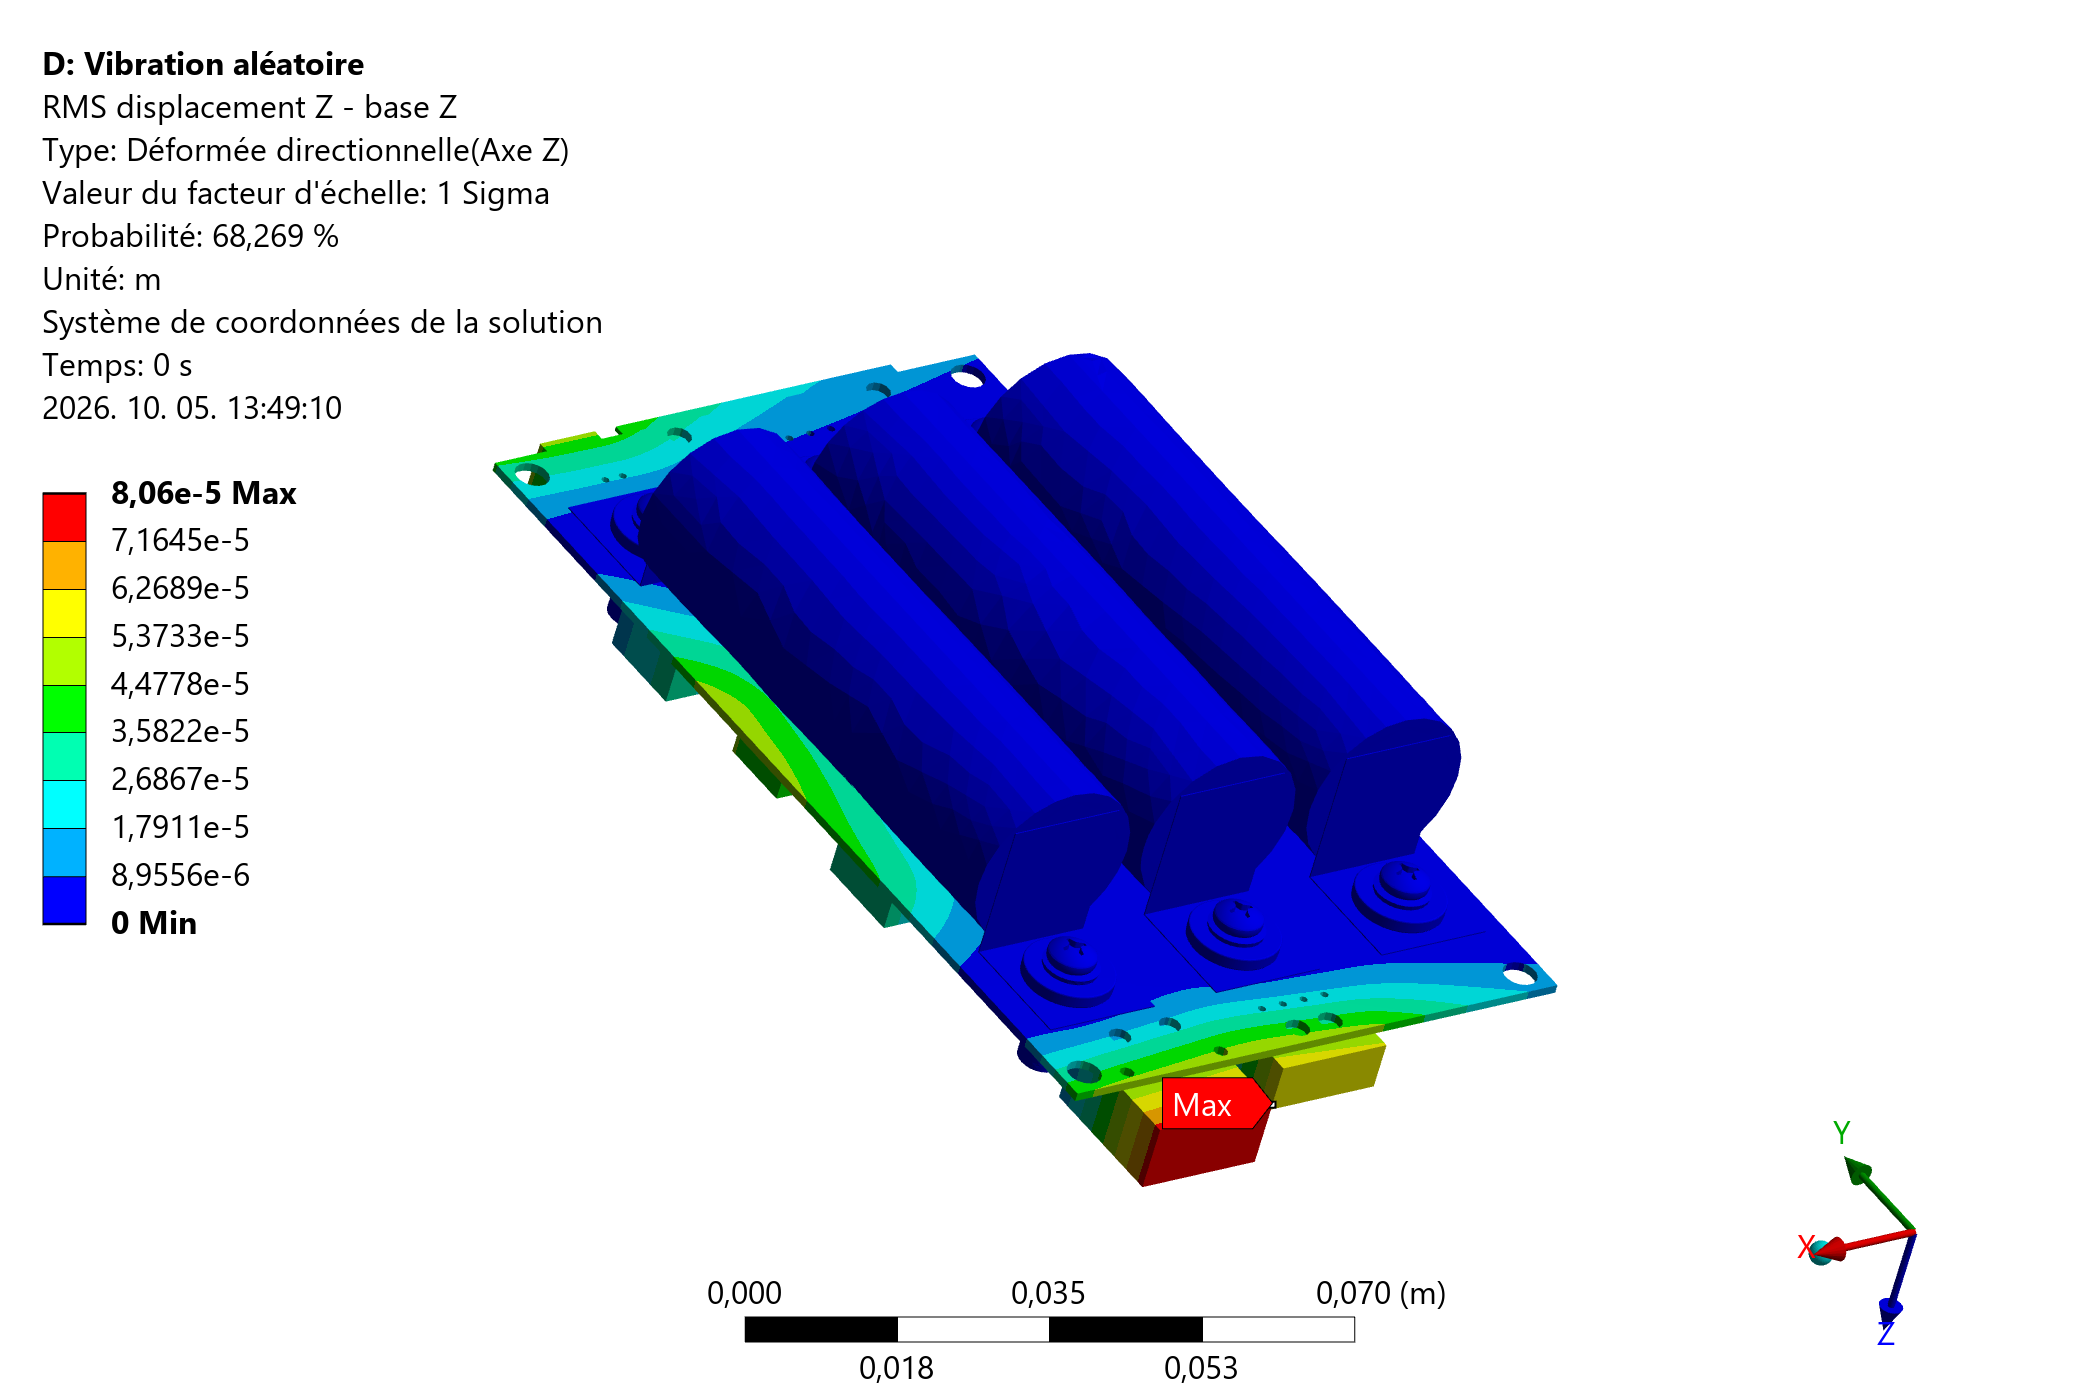
\includegraphics[width=.90\linewidth]{figures/BatteryBaseZResponseZ.png}
\captionof{figure}{Base Z excitation, global Z-direction displacement RMS over the whole assembly. Maximum 0.08060016 mm. One-sigma response; native legend in metres.}\end{center}
The camera exposes the battery cells, their nickel connections and fastening hardware. The electronic components remain included behind the PCB. Automatic deformation scaling illustrates spatial response patterns; an RMS field does not represent a simultaneous instantaneous displacement configuration. The reproduction appendix records the exact camera vectors, export settings and result-object mapping for all nine views.
\clearpage\PageTitle{PCB deformation under X and Y excitation}
\begin{center}
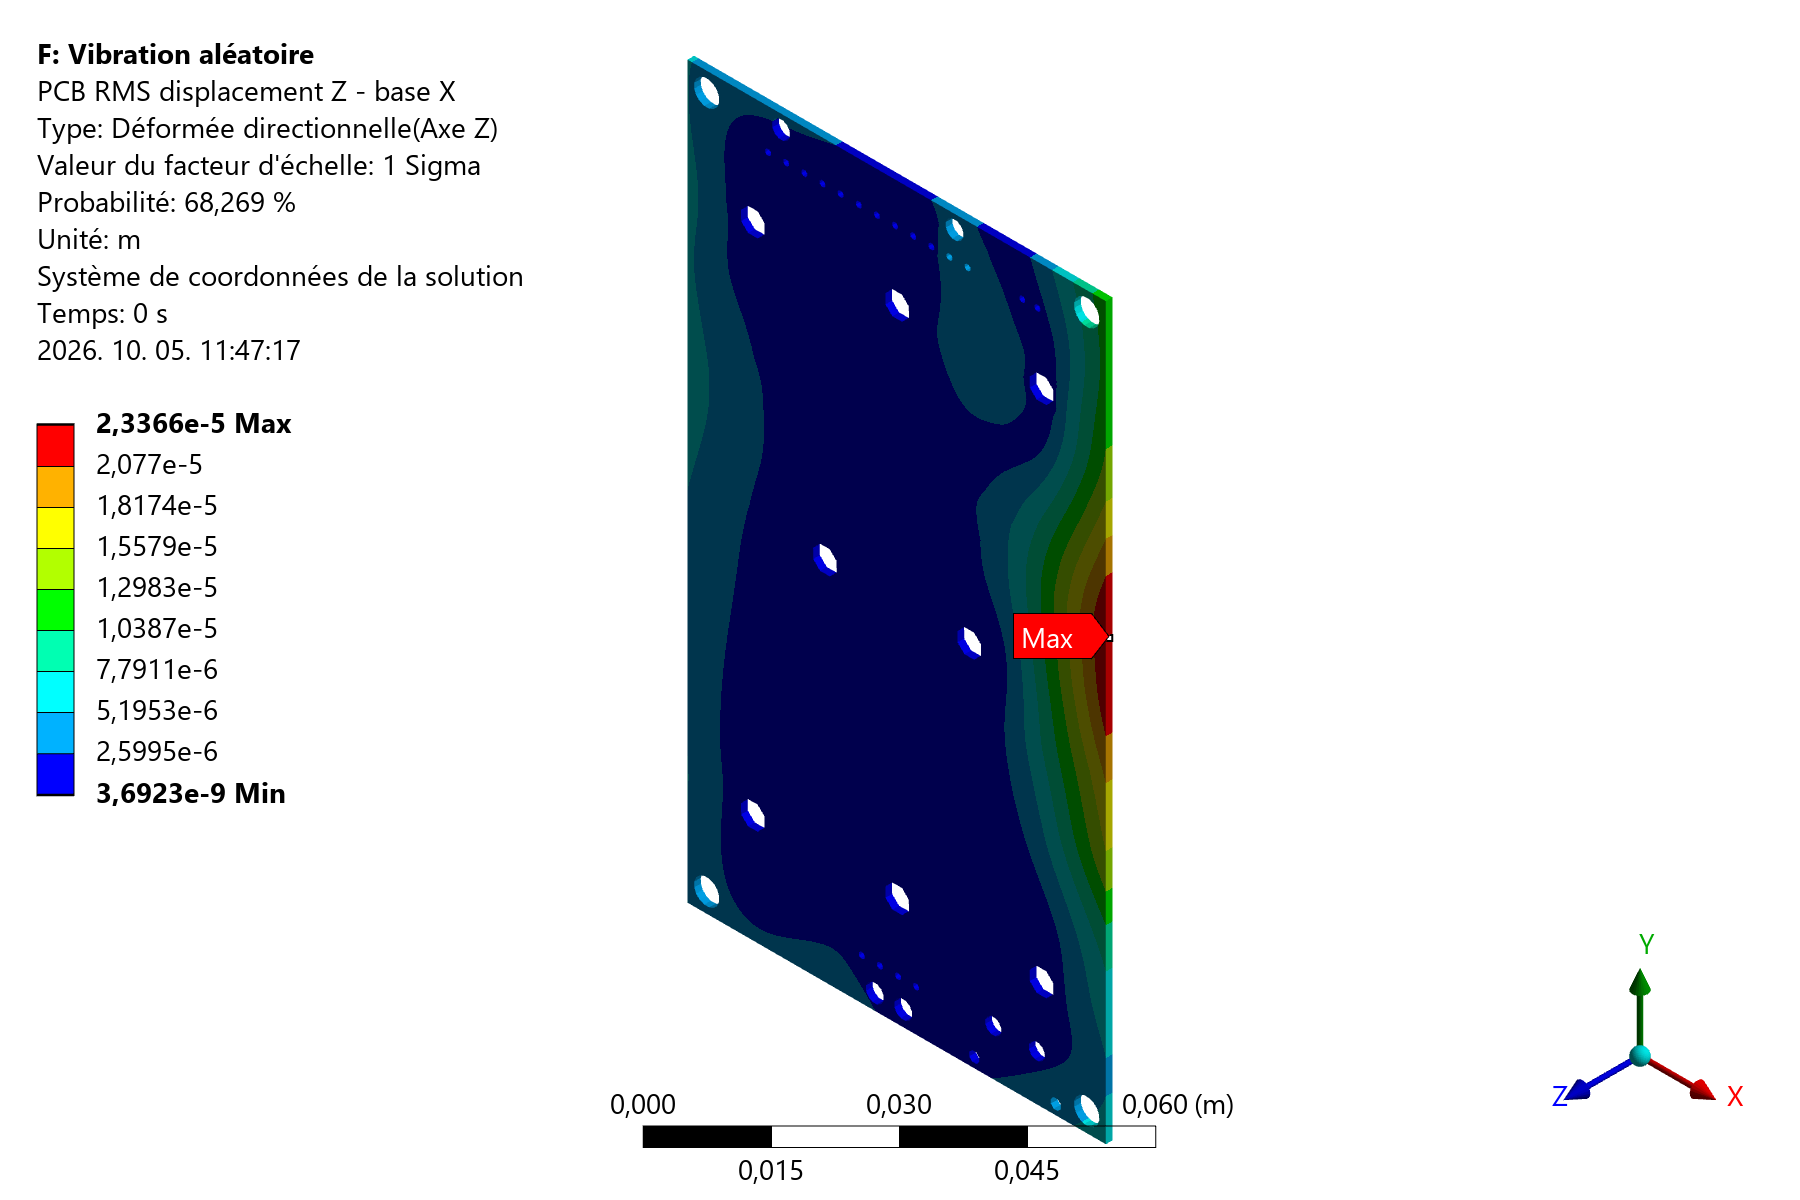
\includegraphics[width=.76\linewidth]{figures/DispX}
\captionof{figure}{X-axis base excitation: PCB Z-direction RMS displacement. Spatial maximum 0.023366 mm. ANSYS native result contour; displayed legend uses metres. Colors show a statistical component response, not a modal eigenvector amplitude.}
\end{center}
\begin{center}
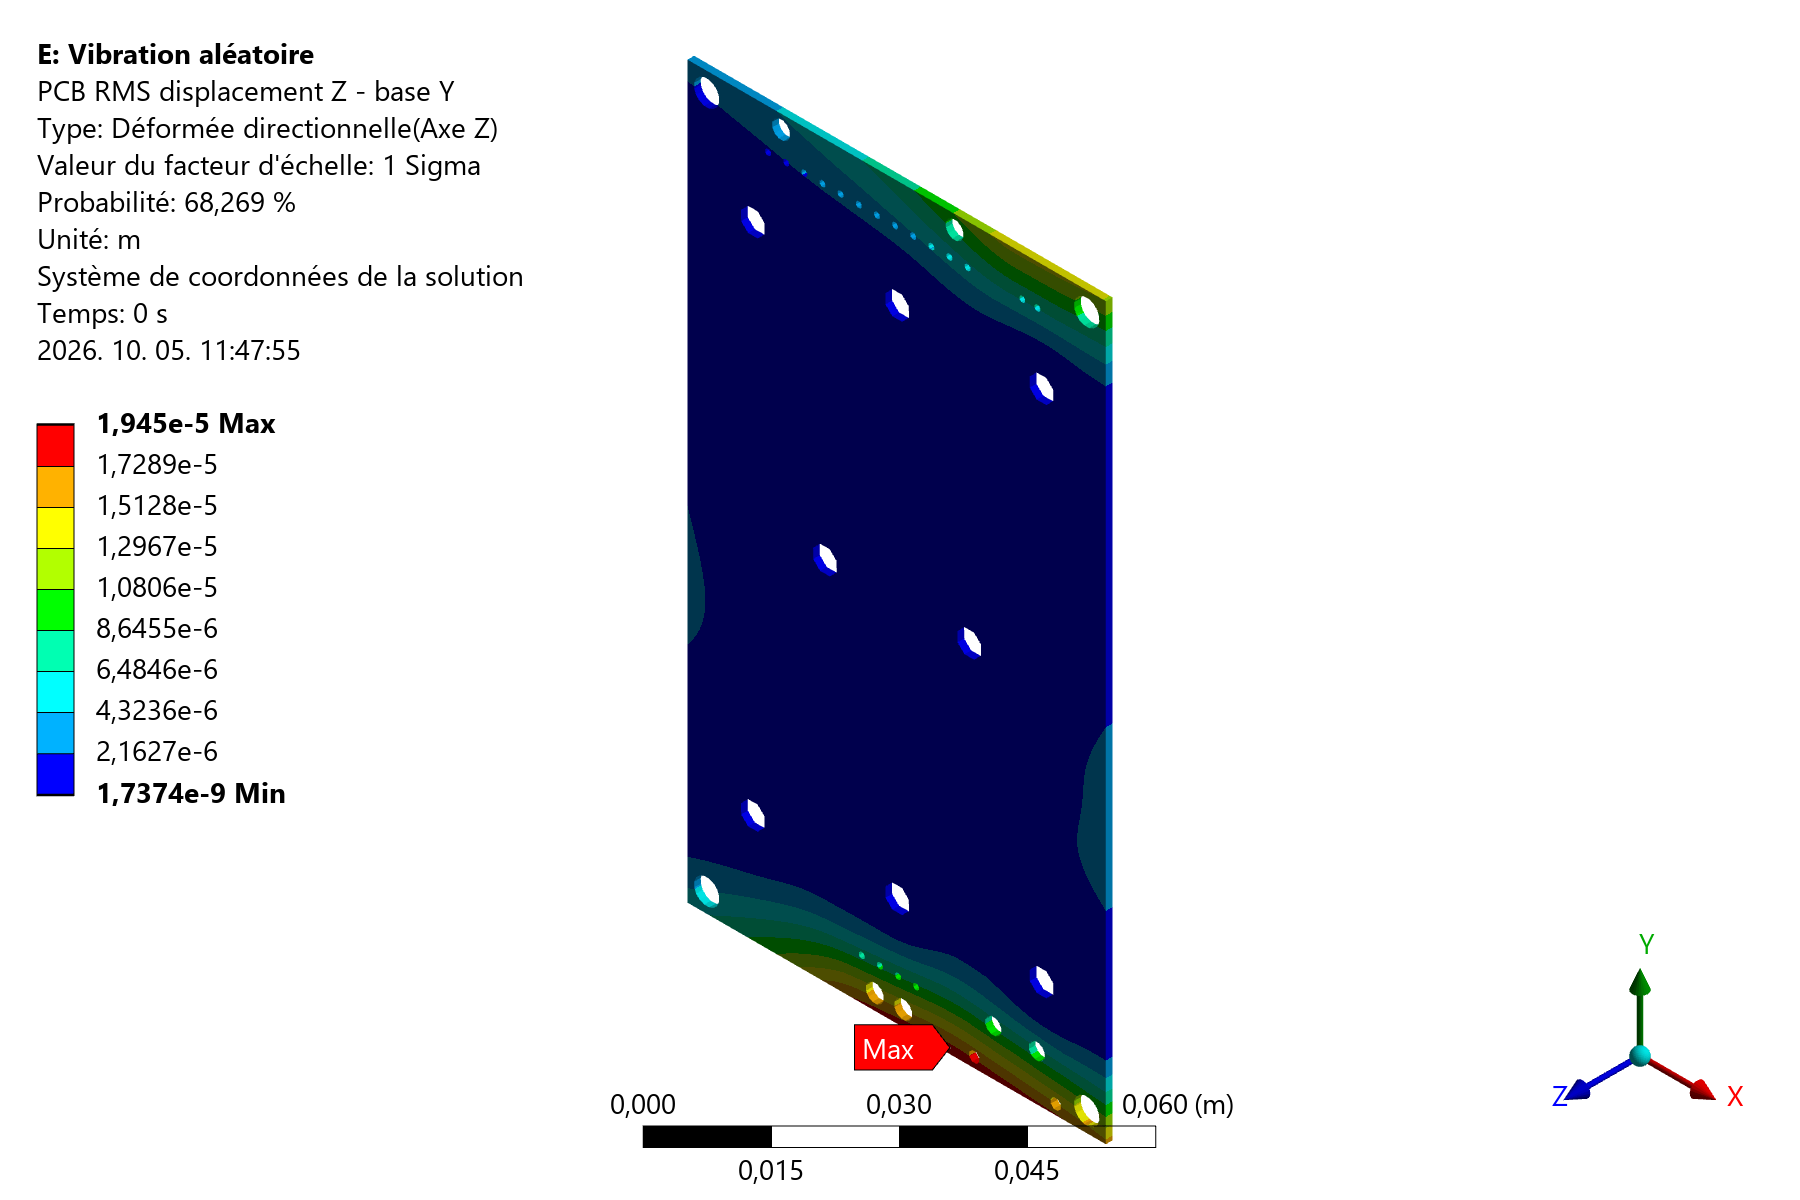
\includegraphics[width=.76\linewidth]{figures/DispY}
\captionof{figure}{Y-axis base excitation: PCB Z-direction RMS displacement. Spatial maximum 0.01945 mm. ANSYS native result contour; displayed legend uses metres. Colors show a statistical component response, not a modal eigenvector amplitude.}
\end{center}
Contours show the largest PCB displacement component for each excitation case. Any displayed geometric deformation is a visualization scale; an RMS field is not an instantaneous deformed configuration.

\clearpage\PageTitle{PCB deformation and stress under random vibration}
\begin{center}
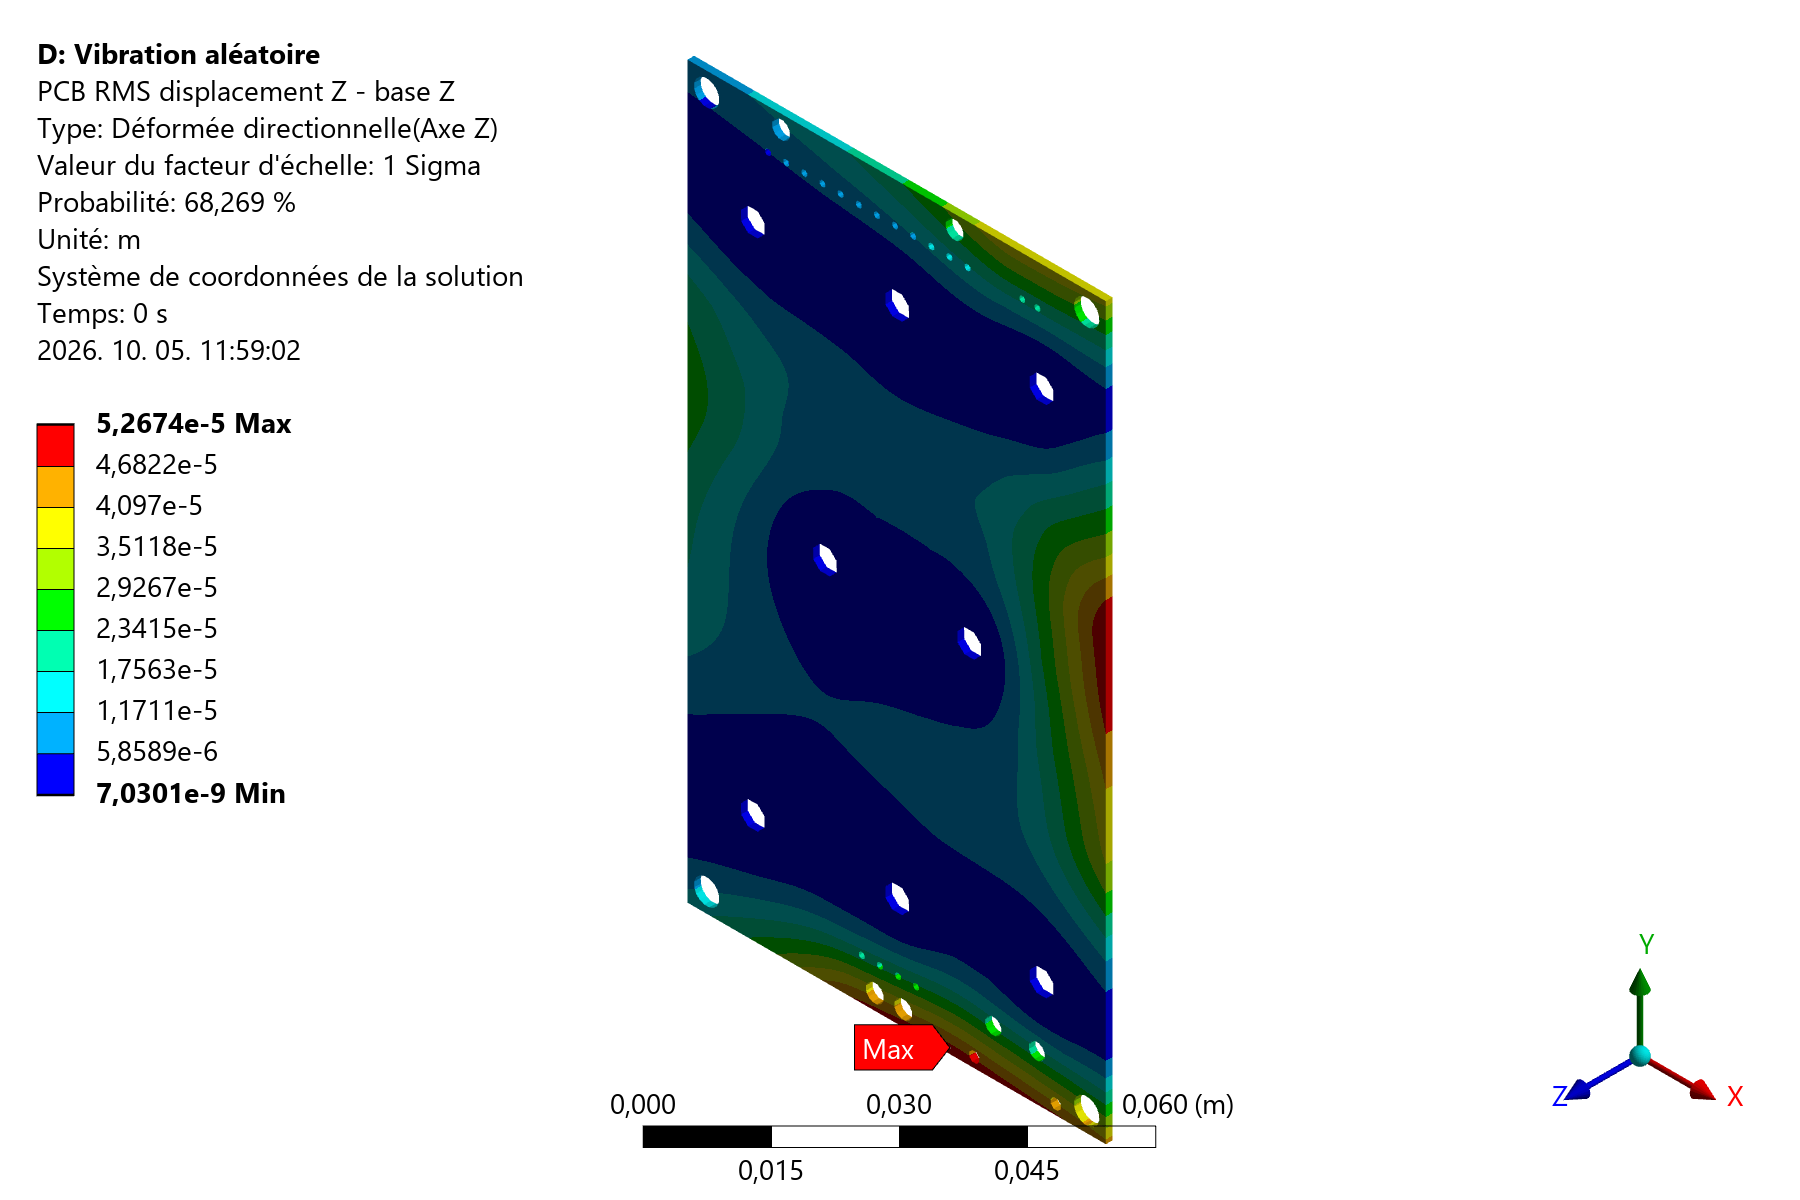
\includegraphics[width=.76\linewidth]{figures/DispZ}
\captionof{figure}{Z-axis base excitation: PCB Z-direction RMS displacement. Spatial maximum 0.052674 mm. ANSYS native result contour; displayed legend uses metres. Colors show a statistical component response, not a modal eigenvector amplitude.}
\end{center}
\begin{center}
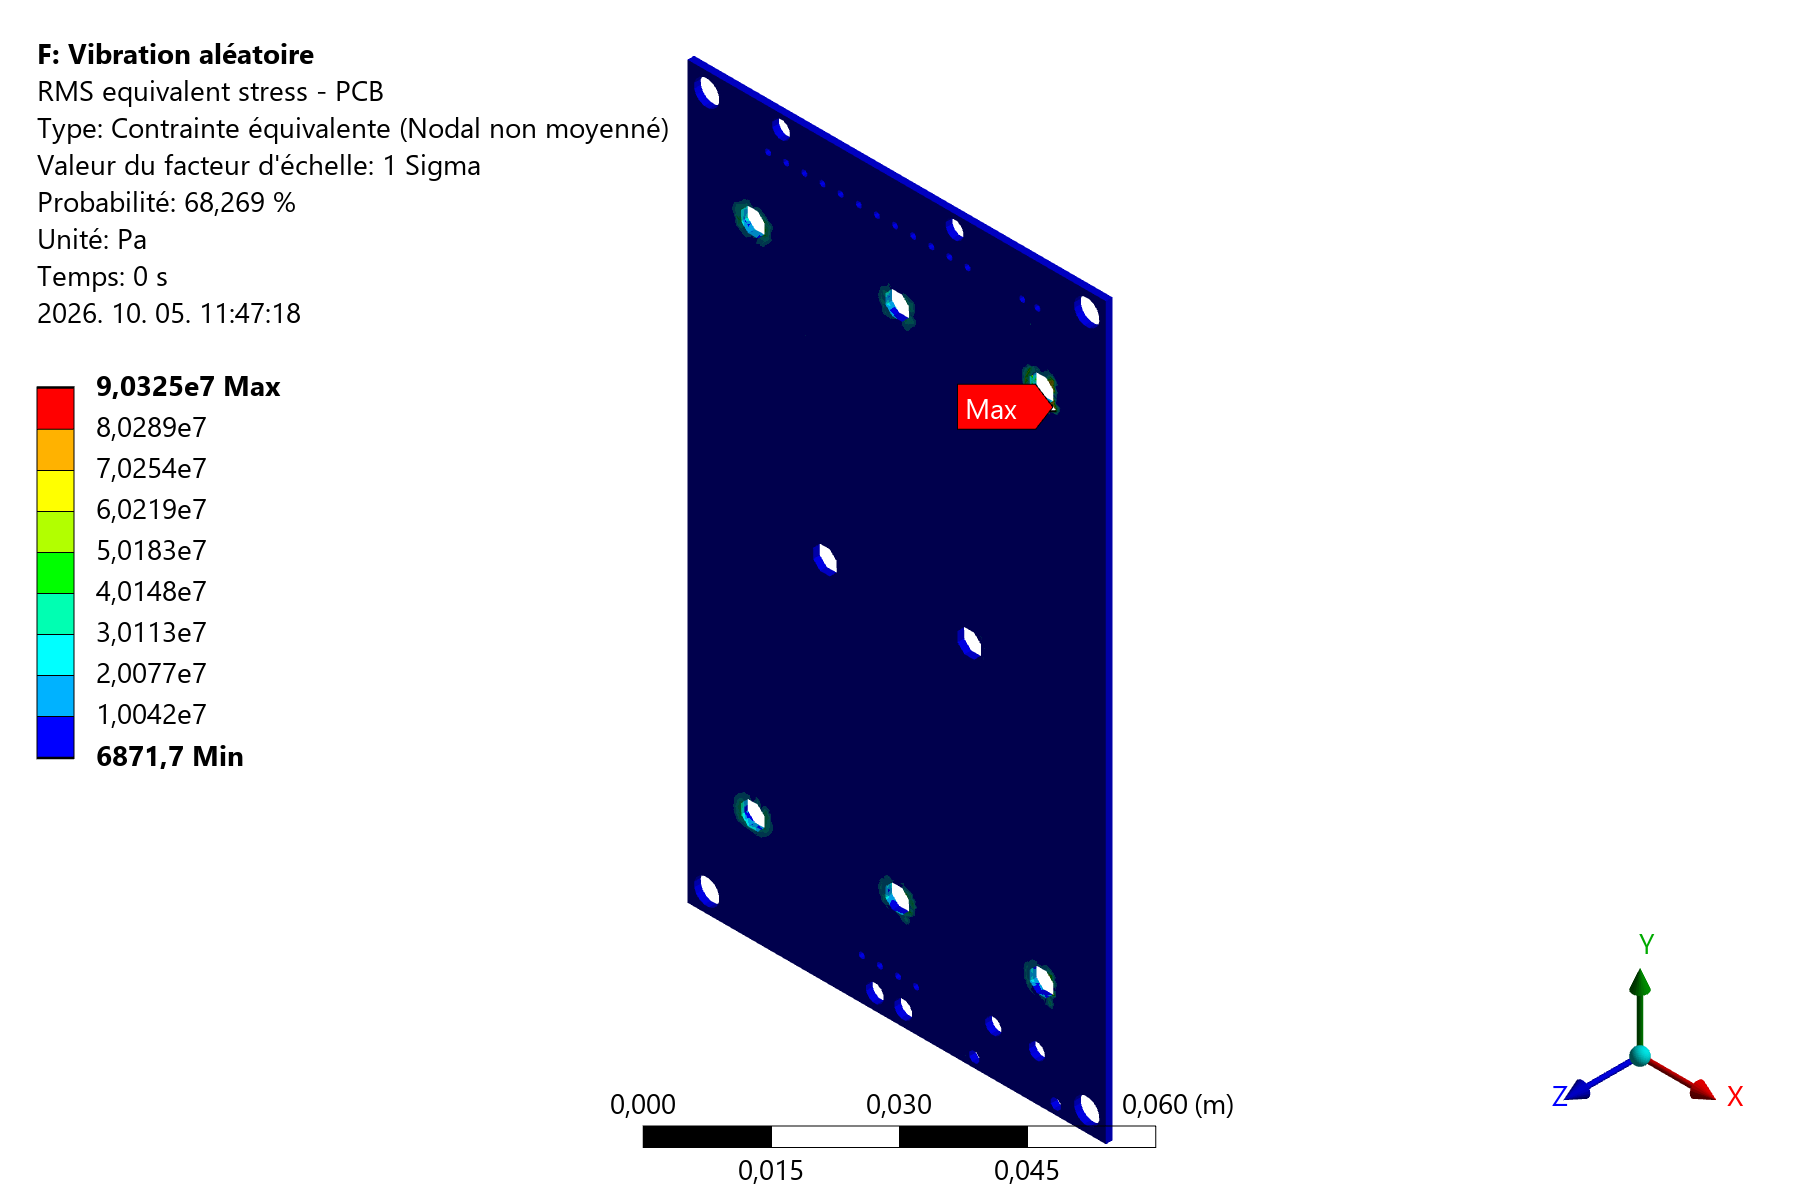
\includegraphics[width=.76\linewidth]{figures/WorstStress}
\captionof{figure}{Highest PCB equivalent-stress RMS occurs for X-axis base excitation: 90.325 MPa. Unaveraged Segalman--Fulcher result. Static clamp stress is separate; the native Gaussian probability label does not apply to equivalent stress.}
\end{center}
\clearpage\PageTitle{Model and numerical checks}
\ReportHeading{Assembly and loading}
The board lies in the global XY plane; Z is normal to the PCB. The same eight mounting faces are fixed, and a single coherent base motion is applied to their 781 mesh nodes in the specified axis. Native checks matched these nodes exactly to the geometry scopes. Standard gravity is 9.80665 m/s²; the four PSD ordinates were converted to SI acceleration²/Hz before solving.

All six bolts inherit the locked equilibrium at static time 2, load step 2, substep 4. Verified locked reactions range from 749.9968 to 749.99945 N. Battery connections remain limited to the nickel strips; no battery-to-PCB bond was added.

\ReportHeading{Mesh and modal basis}
The shared refined quadratic mesh has 368,754 geometry-mesh nodes and 112,902 solid elements across 208 bodies. The solver has additional contact and pretension entities. PCB sizing is 0.7 mm and bolt sizing is 0.4 mm. This random-vibration study did not change that mesh.

The modal extraction is undamped, starts at 1 Hz, and requests up to 60 modes through 4000 Hz. There are 38 modes in that interval. The first 20 frequencies match the accepted earlier bolt study to the exported precision. Stress and strain recovery were enabled before this solve.

\ReportHeading{Numerical checks}
The modal solve completed with zero errors. Extracted translational effective-mass fractions are X 87.24\%, Y 89.04\% and Z 89.56\%. The frequency range exceeds 1.5 times the 2000 Hz PSD limit, but a modal-basis convergence study has not been established.

Each random case passed a native input check without PFACT or SOLVE, followed by an authorized solve. Input hashes, damping, spectrum ordinates, mounting nodes, solver completion and complete finite response fields were checked. All 781 supports reproduce the prescribed 14.136 g RMS acceleration in each case. No insignificant modes were excluded. Velocity and absolute acceleration were retained alongside relative displacement.

\ReportHeading{Highest assembly stress location}
The greatest assembly stress occurs under X-axis excitation in CAD body Part 24[1] (geometry ID 20466). Its exported maximum is at node 29373, element 7017. This localized fastener-model result requires validation before it can support a strength judgment.

\begin{center}
\begin{tabular}{c r r r r}
\toprule
\textbf{Case} & \textbf{Errors} & \textbf{Warnings} & \textbf{Finite fields} & \textbf{Support nodes} \\
\midrule
X & 0 & 22 & 17 / 17 & 781 / 781 \\
Y & 0 & 22 & 17 / 17 & 781 / 781 \\
Z & 0 & 22 & 17 / 17 & 781 / 781 \\
\bottomrule
\end{tabular}
\end{center}
The three input decks were compared and differ only in excitation axis, analysis title and runtime location. Inherited warnings remain part of the qualification limits below.

\clearpage\PageTitle{Prestressed modal basis}
\begin{center}
\begin{tabular}{r r r r}
\toprule
\textbf{Mode} & \textbf{Frequency (Hz)} & \textbf{Mode} & \textbf{Frequency (Hz)} \\
\midrule
1 & 485.964 & 20 & 2364.179 \\
2 & 596.964 & 21 & 2369.941 \\
3 & 645.435 & 22 & 2537.213 \\
4 & 781.350 & 23 & 2704.288 \\
5 & 820.242 & 24 & 2874.956 \\
6 & 826.296 & 25 & 2923.998 \\
7 & 1122.018 & 26 & 2950.883 \\
8 & 1139.112 & 27 & 3016.715 \\
9 & 1199.708 & 28 & 3201.733 \\
10 & 1366.076 & 29 & 3237.676 \\
11 & 1467.900 & 30 & 3368.526 \\
12 & 1714.134 & 31 & 3460.285 \\
13 & 1941.548 & 32 & 3551.455 \\
14 & 2003.039 & 33 & 3597.699 \\
15 & 2017.959 & 34 & 3654.570 \\
16 & 2135.663 & 35 & 3692.040 \\
17 & 2183.755 & 36 & 3775.152 \\
18 & 2212.560 & 37 & 3911.142 \\
19 & 2301.314 & 38 & 3986.075 \\
\bottomrule
\end{tabular}
\end{center}
\begin{center}\begin{minipage}{.86\linewidth}% Editable native PGFPlots figure. Data are plain numerical CSV files.
\begin{tikzpicture}
\begin{axis}[
 width=.985\linewidth,height=6.4cm,xmin=0,xmax=4000,ymin=0,ymax=100,
 xlabel={Frequency (Hz)},ylabel={Cumulative effective mass (\%)},
 xtick={0,500,1000,1500,2000,2500,3000,3500,4000},
 ytick={0,20,40,60,80,100},grid=major,grid style={gray!20},
 tick label style={font=\footnotesize},label style={font=\footnotesize},
 scaled ticks=false,legend pos=south east,
 legend style={font=\scriptsize,draw=gray!35,fill=white,cells={anchor=west}}]
\path[fill=Teal,fill opacity=0.08] (axis cs:20,0) rectangle (axis cs:2000,100);
\addlegendimage{area legend,draw=Teal!30,fill=Teal!8}
\addlegendentry{Input PSD range}
\addplot[const plot,color=orange!80!black,line width=1pt] table[x=frequency_hz,y=cumulative_mass_percent,col sep=comma]{data/modal_mass_X.csv};
\addlegendentry{X: 87.24\% retained}
\addplot[const plot,color=Teal,line width=1pt] table[x=frequency_hz,y=cumulative_mass_percent,col sep=comma]{data/modal_mass_Y.csv};
\addlegendentry{Y: 89.04\% retained}
\addplot[const plot,color=Navy,line width=1pt] table[x=frequency_hz,y=cumulative_mass_percent,col sep=comma]{data/modal_mass_Z.csv};
\addlegendentry{Z: 89.56\% retained}
\end{axis}
\end{tikzpicture}
\end{minipage}\captionof{figure}{Cumulative modal effective mass as a fraction of total directional mass. The shaded band is the 20--2000 Hz input range. A frequency cutoff alone does not establish response convergence.}\end{center}
\clearpage\PageTitle{Qualification and traceability}
\ReportHeading{Exploratory assumptions}
The 2\% damping ratio was selected by the user as an exploratory assumption; no damping measurement was supplied. Peak response near resonance is damping-sensitive. This report does not establish a damping uncertainty interval.

Inherited isotropic PCB properties are E = 23.33024 GPa, Poisson ratio 0.15 and density 1969.7774 kg/m³. Batteries use a homogeneous E = 200 GPa, Poisson ratio 0.3 and density 2200 kg/m³. These idealizations have not been correlated with the actual board laminate or cell construction.

\ReportHeading{Contact and stress limitations}
The bolt model uses existing solid shafts with pretension cuts and MPC shaft-to-hole connections. Washer-to-PCB frictionless seats use Adjust to Touch to bridge a 0.746 mm CAD gap. This is an assumed assembled seating condition. The random response is linearized about the locked state; it does not predict contact opening, slip transitions or bolt loosening.

The inherited model contains thin nickel-strip mesh-quality warnings, including highly distorted tetrahedra, and hardware constraint-overlap warnings. The expanded modal solve reports 2251 warnings, including inherited shape warnings and repeated ACT parameter definitions. These warnings have not been eliminated.

The static model previously produced a peak elastic equivalent stress of approximately 1.142 GPa. That localized value and the random stress maxima require mesh, contact and material validation before any strength conclusion. The static mean and random equivalent-stress RMS must not be added as if they were compatible stress tensors.

\ReportHeading{Statistical interpretation}
RMS displacement and acceleration characterize stationary zero-mean vibration. Three-sigma scaling is an estimate of excursions at a point, not a guaranteed maximum over a test or flight. Equivalent stress uses a non-Gaussian statistical measure. The generic 68.269\% / 1-sigma label on native ANSYS equivalent-stress plots must not be interpreted as a Gaussian coverage probability. A displayed time of 0 s is the stored result-set label, not an instantaneous vibration state. No test duration, fatigue law or acceptance limits were supplied, so no fatigue life or pass/fail margin is claimed.

\ReportHeading{Evidence and reproducibility}
The preserved run is outputs/random\_vibration\_20261005\_0950. It contains the input specification, native input decks, preflight logs, modal participation tables, solver logs, CSV/TSV result tables, and ANSYS contour images. Expanded modal analysis ID: 4254. Random analysis IDs: X 4259, Y 4264, Z 4269.

Solver: ANSYS Mechanical/MAPDL 2026 R1.02, build 26.1 UP20260202, Windows 11 in Parallels; 12 distributed processes. Each random case was solved in an isolated Windows runtime, archived with SHA-256 hashes, and imported into its Mechanical analysis by reference for field recovery. This recovered a Mechanical result-handoff failure; the accepted numerical solutions have zero solver errors. The source project remains powerboardsim\_v1.wbpj. The prior default-contact/modal comparison is preserved separately. The report source keeps ANSYS contours as external PNG files and draws both graphs using editable native PGFPlots code and numerical data tables.

\ReportHeading{References}
\begin{enumerate}
\item \href{https://ansyshelp.ansys.com/public/Views/Secured/corp/v261/en/wb_sim/ds_spectral_analysis_type.html}{ANSYS Mechanical 2026 R1: Random Vibration Analysis}.
\item \href{https://ansyshelp.ansys.com/public/Views/Secured/corp/v261/en/ans_thry/thy_anproc7.html}{ANSYS Theory Reference 2026 R1: Spectrum Analysis}.
\item \href{https://ansyshelp.ansys.com/public/Views/Secured/corp/v261/en/ans_cmd/Hlp_C_PSDUNIT.html}{ANSYS 2026 R1: PSDUNIT and excitation units}.
\item \href{https://ansyshelp.ansys.com/public/Views/Secured/corp/v261/en/ans_cmd/Hlp_C_PSDGRAPH.html}{ANSYS 2026 R1: Input PSD curve-fit display}.
\end{enumerate}
}


% Reproduction appendix, verified against archived run evidence.
\usepackage{listings,xurl}
\lstset{basicstyle=\ttfamily\fontsize{8}{9.7}\selectfont,
 breaklines=true,breakatwhitespace=false,columns=fullflexible,
 keepspaces=true,showstringspaces=false,upquote=true,
 frame=single,rulecolor=\color{Teal!40},backgroundcolor=\color{Teal!3},
 xleftmargin=3pt,xrightmargin=3pt,aboveskip=6pt,belowskip=6pt}
\newcommand{\ReproPage}[1]{\clearpage\phantomsection
 \addcontentsline{toc}{section}{#1}\PageTitle{#1}}

\begin{document}
\ReportBody

\clearpage
\PageTitle{Reproduction procedure}
This appendix records the accepted workflow and the files needed to repeat it. It was added on 5 October 2026 by checking the saved Mechanical commands, native input decks, solver logs and result audits. The existing numerical results have not been changed or re-solved for this documentation revision.

\textbf{Starting point.} Use a copy of the complete saved Workbench project and its companion project directory. The ECAD archive alone does not contain this assembled mechanical model, its added battery hardware, its inherited materials, or the established contact scopes. Exact numerical replay uses the supplied native decks; rebuilding from imported geometry can change entity IDs, mesh and results.

\textbf{How to follow the appendix.} Follow the numbered sections in order. Code is explicitly labelled as Mechanical IronPython, Windows PowerShell, MAPDL, or report-build commands. Replace only the stated paths and fresh output names. Retain the accepted evidence folders. The code excerpts are instructions reconstructed from executed commands, not a newly tested one-click installer. Full original helper scripts are supplied as references; some contain historical paths, global variables, or one-run guards and must not be launched blindly.

The source bundle contains a \path{reproduction/} directory with native inputs, contact/body inventories, custom bolt-library files, selected original scripts, acceptance evidence and a SHA-256 manifest. Large binary solution/restart files and the complete CAD/Workbench project are retained separately in the project tree, not duplicated in the report ZIP. Their dependencies are identified below.

\begingroup\small\setlength{\parskip}{0pt}
\renewcommand{\contentsname}{Procedure index}
\tableofcontents
\endgroup

\ReproPage{1. Preserve the project and establish the environment}
\begin{enumerate}
\item Close or save Mechanical, then copy the entire project folder to a new study folder. Keep \path{powerboardsim_v1.wbpj}, \path{powerboardsim_v1_files/}, and \path{outputs/} together. Open the copied project in Workbench and open its Model cell in Mechanical. Do not substitute a lone old \path{SYS.mechdb} into the current project: saved model files are snapshots, not complete portable projects.
\item Use ANSYS Mechanical/MAPDL 2026 R1.02, build 26.1 UP20260202. The accepted solver used 12 distributed processes. The original VM was Windows 11 in Parallels with 14 virtual CPUs and 112 GB RAM. Keep enough local disk space for per-rank matrices and results: one random-case staging copy was approximately 25 GB before new results.
\item Load the existing APDL Bolt Manager extension (internal extension name \texttt{BoltTools}, version 2024.1). Sherlock's imported geometry and material assignments must already be present. The accepted export also identifies Sherlock\_App 2026.1. Use solver units m, kg, s, N; the geometry and mesh sizing tables below are in mm.
\item Establish a new output folder. In the original project, call the project root \texttt{P}, the accepted modal run \texttt{B}, and the accepted random run \texttt{R}, using the paths below. A fresh rerun must use different output directories. Do not reuse completion markers from an old run as evidence that a new run passed.
\end{enumerate}

\begin{lstlisting}
# Original Windows project root (Z: maps the macOS user home):
P = r'Z:\Developer\MIT_Rkt_Team\2026-7\MIT-RT-26_27-Work\simulation_work\avionics\powerboardsim\1'
B = P + r'\outputs\bolt_manager_work\resume_20261005_004228'
R = P + r'\outputs\random_vibration_20261005_0950'
# Native solver executable:
# C:\Program Files\ANSYS Inc\v261\ansys\bin\winx64\ANSYS261.exe
\end{lstlisting}

\ReportHeading{Identify analyses by their role, then verify their IDs}
\begin{center}\small\begin{tabular}{l r l}\toprule
Role in the saved model & Object ID & Native directory under dp0\\\midrule
Static, 750 N load then lock & 4123 & SYS-2/MECH\\
20-mode prestressed comparison & 1656 & SYS-1/MECH\\
Default comparison, later refined & 4182 & SYS-3/MECH\\
Expanded modal basis for random & 4254 & SYS-4/MECH\\
Random X / Workbench block F & 4259 & SYS-5/MECH\\
Random Y / Workbench block E & 4264 & SYS-6/MECH\\
Random Z / Workbench block D & 4269 & SYS-7/MECH\\\bottomrule
\end{tabular}\end{center}
Object IDs, Workbench letters and folder names can change when objects are recreated. A new study should resolve the corresponding objects and confirm their names, types and upstream links before using any ID from this report. A geometry ID is not a Mechanical object ID.

Open Mechanical's Scripting pane and select its IronPython environment for the snippets below. Use \texttt{System.IO} for files there. The previous \lstinline!ImportError: No module named _json! is avoided by keeping JSON parsing in host Python 3; it is not repaired by changing the material model.

\ReproPage{2. Verify the complete assembly, supports and materials}
\begin{enumerate}
\item Expand Geometry. Verify 208 unsuppressed, meshed bodies, including 172 imported \texttt{COMP\_} electronic-component bodies, three cell bodies, nickel strips, six battery screws, washers and stand-offs. Keep component solids in the solve even when making a PCB-only contour. The assembled mass is approximately 0.25182 kg.
\item Check \path{reproduction/common/assembly_body_inventory.tsv}: it lists each body's geometry ID, Mechanical object ID, material and meshed node/element counts. Match the inventory before altering contacts. PCB geometry ID is 42342 (Mechanical body object 3558); the PCB measures approximately $69.215\times120.777\times1.10236$ mm.
\item Scope one Fixed Support to the eight existing mounting end faces below. In the accepted static analysis its object ID is 4127; the default analysis uses a separate support on the same faces. Do not fix the six battery screws directly, and do not add weak springs to hide a disconnected assembly.
\item Retain the inherited material assignments. Verify elastic stiffness and density in Engineering Data and in the exported native material records. Assigning one generic material to all components would create a different study. The full native decks contain the actual material definitions and their element assignments; the table below only highlights the large structural bodies.
\end{enumerate}
\begin{center}\small\begin{tabular}{l p{106mm}}\toprule
Scope & Geometry entity IDs\\\midrule
Fixed mounting faces & 23075, 23135, 23195, 23255, 23315, 23375, 23435, 23495\\
PCB / underside seat target & Body 42342 / face 41909\\
Battery cells & 20157, 20675, 20822\\
Nickel strips & 20091, 20297, 20348, 20642, 20756, 20929\\\bottomrule
\end{tabular}\end{center}
\begin{center}\small\begin{tabular}{l r r r}\toprule
Stored material & $E$ (Pa) & $\nu$ & $\rho$ (kg/m$^3$)\\\midrule
PCB & 23330241935.4839 & 0.15 & 1969.77741935484\\
PilesLiPo & $2.0\times10^{11}$ & 0.30 & 2200\\
NICKEL-200 & $2.2\times10^{11}$ & 0.305 & 8874\\
Acier standard & $2.0\times10^{11}$ & 0.30 & 7850\\\bottomrule
\end{tabular}\end{center}
\ReportHeading{Initialize the Mechanical API without relying on a previous console session}

\begin{lstlisting}
import System
from Ansys.Core.Units import Quantity
from Ansys.ACT.Interfaces.Common import SelectionTypeEnum
from Ansys.Mechanical.DataModel.Enums import *
m = ExtAPI.DataModel.Project.Model
static = ExtAPI.DataModel.GetObjectById(4123)
bolted = ExtAPI.DataModel.GetObjectById(1656)
ext = [x for x in ExtAPI.ExtensionManager.Extensions
       if x.Name == 'BoltTools'][0]
manager = [x for x in ExtAPI.DataModel.GetUserObjects(ext)
           if x.Name == 'ApdlBoltManager'][0]
bm = ext.GetModule().ApdlBoltModule
def sel(ids):
    s = ExtAPI.SelectionManager.CreateSelectionInfo(
        SelectionTypeEnum.GeometryEntities)
    s.Ids = list(ids)
    return s
def enumset(obj, name, value):
    p = obj.GetType().GetProperty(name)
    p.SetValue(obj, System.Enum.Parse(p.PropertyType, value), None)
\end{lstlisting}

\ReproPage{3. Restore the intended contacts and refined mesh}
\begin{enumerate}
\item Preserve the existing contact definitions and scopes. Do not run automatic contact generation as a reproduction step: that was previously capable of changing pairings. The accepted bolted network has 210 active contact regions: 172 component-to-PCB bonds, 8 stand-off-to-PCB bonds, 24 hardware/nickel/battery bonds, and 6 frictionless bearing seats. Additional shaft-to-hole MPC elements are generated by the bolt extension.
\item Enforce the user's battery rule: only battery-to-nickel connections are active. The six allowed contact regions are listed below. Suppress any battery-to-PCB, battery-to-washer or other direct battery contact. Do not replace them with frictionless battery-to-PCB contact; even that would introduce an extra load path. Check for shared mesh nodes as well as contact objects.
\item For the refined models, set the 172 component-to-PCB bonds to Asymmetric, MPC, Nodal Normal to Target. Component faces are the contact/source side; PCB faces are the target side. Retain the detailed face scopes from the saved project. \path{reproduction/common/final_active_contacts.tsv} records body-level pairs; the native decks preserve the exact meshed contact surfaces.
\item In Mesh, retain existing controls and set Element Order to Quadratic. Add or edit body sizing: PCB body 42342 at 0.7 mm; screw bodies 21279, 21629, 21979, 22329, 22679, 23029 at 0.4 mm. Generate the mesh. Expected geometry mesh: 368754 nodes and 112902 solid elements; PCB alone: 217704 nodes and 39014 elements. Remeshing in a different release can change this mesh. Use the archived decks for identical node/element replay.
\item Insert the following Commands object into the static analysis and the refined-default modal analysis. Keep legacy Commands object 4113 suppressed. Preserve the export order so that the command executes before SOLVE. The original unrefined default did not receive this numerical correction.
\end{enumerate}

\begin{lstlisting}
FINISH
/PREP7
ETCONTROL,OFF
SHPP,WARN
FINISH
/SOLU
\end{lstlisting}

\begin{center}\small\begin{tabular}{r r r l}\toprule
Contact object & Source body & Target body & Accepted type\\\midrule
1699 & 20091 & 20157 & Bonded\\
1711 & 20157 & 20348 & Bonded\\
1726 & 20297 & 20675 & Bonded\\
1753 & 20642 & 20675 & Bonded\\
1759 & 20756 & 20822 & Bonded\\
1768 & 20822 & 20929 & Bonded\\\bottomrule
\end{tabular}\end{center}
In Mechanical, set \texttt{PCB670\_RUN} to a fresh audit directory and run the supplied script \path{reproduction/common/audit_battery_constraints.py}. It checks the six allowed contact pairs and rejects shared nodes between batteries and any non-nickel body. It writes a contact inventory; it does not solve.

The accepted mesh still has 1498 tetrahedra with shape warnings, mostly in nickel, with maximum reported aspect ratio 216.3. Reproducing those warnings is traceability, not a validation target. Mesh improvement would be a new study. The refined comparison also changes integration/contact numerics and therefore is not a pure mesh-convergence experiment.

\ReproPage{4. Configure the six APDL Bolt Manager definitions}
\begin{enumerate}
\item Use the six existing flexible solid screws. Keep the saved APDL Bolt Manager and its six children; do not add six additional geometric screws or duplicate pretension objects. Child IDs in the accepted project are 4139, 4147, 4155, 4163, 4171 and 4179. The manager ID is 4122.
\item Make the three files in \path{reproduction/custom_library/} available in BoltTools' configured custom-part library and reload it with \texttt{bm.LoadXmlApdlBolts()}. Check that \path{bm.ApdlBoltDict['PCB_ExistingBolt_670N.xml'].LoadErrors} is empty. The old \texttt{670N} filename is retained for compatibility; its \textbf{actual stored load is 750 N}. Do not change it back to 670 N.
\item For each row below, create or verify three geometry Named Selections: \texttt{PCB670\_nn\_BODY}, \texttt{PCB670\_nn\_SHAFT}, \texttt{PCB670\_nn\_HOLE}. Send them to the solver as node components. Use the reported body and faces, not all shaft-adjacent parts. The exported body component is selected as elements in the custom preprocessor commands.
\item Verify a global-aligned coordinate system at each listed $x,y$ and $z=-3.772678375$ mm. On each Bolt Manager child, select that one coordinate system; set the bolt part to the custom XML; set Bolt Washer, Nut and Nut Washer to None; set Display/Visible to No. The custom definition adds pretension/contact elements to existing solids rather than extra bolt mass.
\end{enumerate}
\begin{center}\small\begin{tabular}{r l r l l}\toprule
No. & Position & Body & Shaft faces & PCB hole faces (inclusive)\\\midrule
1 & Left, high Y & 21279 & 21214, 21273 & 41970--41977\\
2 & Centre, high Y & 21629 & 21564, 21623 & 41962--41969\\
3 & Right, high Y & 21979 & 21914, 21973 & 41954--41961\\
4 & Left, low Y & 22329 & 22264, 22323 & 41914--41921\\
5 & Centre, low Y & 22679 & 22614, 22673 & 41922--41929\\
6 & Right, low Y & 23029 & 22964, 23023 & 41930--41937\\\bottomrule
\end{tabular}\end{center}
\begin{center}\small\begin{tabular}{r r r}\toprule No. & $x$ (mm) & $y$ (mm)\\\midrule
1 & 10.81234895 & 102.90699896\\2 & 34.81234887 & 102.90699896\\3 & 58.81234883 & 102.90699896\\
4 & 10.81234894 & 17.90699886\\5 & 34.81234886 & 17.90699886\\6 & 58.81234882 & 17.90699886\\\bottomrule\end{tabular}\end{center}
Each child's User Commands entry is sent at Assembly level for the Bolt part, in both Pre and Solve phases. For bolt 1, use the following text; change the index and the three solver names for each successive bolt.

\begin{lstlisting}
PBIndex=1
PBBody='PCB670_01_BODY'
PBShaft='PCB670_01_SHAFT'
PBHole='PCB670_01_HOLE'
\end{lstlisting}

The API representation is \texttt{obj.Attributes['UserCmds']} containing \lstinline![['Existing solid bolt scopes', text, ['Pre','Solve'], ['Bolt'], ['Assembly']]]!. After editing, call \path{obj.Controller.GetData(obj,False)} and \texttt{obj.NotifyChange()}. The bundled historical setup script shows the full API construction, but its old 670 N assumptions and empty-manager checks must not be replayed on the final project.

\ReproPage{5. Define the seats and the load--lock sequence}
\begin{enumerate}
\item For the bolted configuration, unsuppress all six Bolt Manager children. Suppress four incidental washer/stand-off bonds: 1696, 1732, 1744, 1771. Create or unsuppress the six bearing contacts below, with washer as contact/source and PCB underside 41909 as target.
\item Set each bearing contact to Frictionless, Asymmetric, Augmented Lagrange, Pinball Region = Radius, Pinball Radius = 1 mm, Interface Treatment = Adjust to Touch. This deliberately closes the approximately 0.7459997 mm CAD gap. It is the accepted seating assumption; confirm its physical validity separately.
\item In Static Structural, use two steps ending at 1 s and 2 s. Set Large Deflection = On, Weak Springs = Off, Automatic Time Stepping = On for both steps, Initial Substeps = 5, Minimum = 1, Maximum = 100. These times index a quasi-static loading sequence; they are not a vibration duration. Preserve restart data for the downstream modal calculation.
\item The custom XML uses global cut plane \texttt{PBCutZ=-2 mm}, upper shaft range \texttt{PBTopZ=-1 mm} to \texttt{PBMaxZ=2 mm}, and MPC pinball \texttt{PBPinb=1.5 mm}. \texttt{PCB\_ExistingBolt\_Pre.inp} uses PSMESH/PRETS179 and TARGE170/CONTA174. It reserves 2000 node and element IDs per bolt and tests that the cut, target and contact selections are nonempty. Keep the entire supplied file unchanged for exact replay.
\end{enumerate}
\begin{center}\small\begin{tabular}{r r r r r}\toprule
Seat & Contact object & Washer body & Washer face & PCB face\\\midrule
1&4224&20246&20234&41909\\2&4228&20040&20028&41909\\3&4232&20525&20513&41909\\
4&4236&20466&20454&41909\\5&4240&20878&20866&41909\\6&4244&20407&20395&41909\\\bottomrule
\end{tabular}\end{center}
\ReportHeading{Exact load-phase commands in the custom library}
The following is the operative content of \texttt{PCB\_ExistingBolt\_Load.inp}. \texttt{PBLoad} is supplied as 750 N by the XML. The analysis-type guard prevents applying static tightening again during modal or PSD solves.

\begin{lstlisting}
! Static step 1: tensile preload. Step 2: lock achieved adjustment.
! Prestressed modal obtains the locked state from its linked static solution.
*GET,PBAnalysis,ACTIVE,0,ANTY
*IF,PBAnalysis,EQ,0,THEN
PBPN=PBPilot%PBIndex%
*IF,_MechAnalysisStep,EQ,1,THEN
F,PBPN,FX,PBLoad
/COM,PCB_BOLT_%PBIndex% PRELOAD %PBLoad% N
*ELSEIF,_MechAnalysisStep,GT,1,THEN
FDELE,PBPN,FX
D,PBPN,UX,%_FIX%
/COM,PCB_BOLT_%PBIndex% LOCK
*ENDIF
*ENDIF
ALLSEL,ALL
\end{lstlisting}

The \texttt{UX} degree of freedom here belongs to a PRETS179 pretension pilot and represents relative tightening, not an instruction to move the physical screw in global X. Step 1 applies force; step 2 removes that force and locks the achieved adjustment with \texttt{\%\_FIX\%}. Keep this sequence; leaving 750 N force-controlled in step 2 would be a different tangent-state model.

\ReproPage{6. Preflight, solve and verify the static parent}
\begin{enumerate}
\item In Mechanical, export a fresh static native deck after refreshing the ACT writer. Use a new folder. The commands below assume \texttt{newout} is an existing Windows directory and that section 2 initialized the API objects.
\end{enumerate}

\begin{lstlisting}
bm.StartApdlInputFileWrite(static)
static.WriteInputFile(newout + r'\static_input.dat')
s = System.IO.File.ReadAllText(newout + r'\static_input.dat')
assert s.count('PBLoad = 750.0') == 12  # six bolts, two steps
assert s.count('CMSEL,S,%PBBody%,ELEM') == 6
assert 'ETCONTROL,OFF' in s
assert '*GET,PBAnalysis,ACTIVE,0,SOLU,ANTYPE' not in s
\end{lstlisting}

\begin{enumerate}\setcounter{enumi}{1}
\item Run a separate no-SOLVE preflight on a copy of the exported input, truncated immediately before its first standalone \texttt{SOLVE} command. The supplied \path{reproduction/native/static750/preflight.dat} is the exact accepted preflight deck and ends in inventories, \texttt{CNCHECK,DETAIL} and \texttt{/EXIT,NOSAVE}. Use it unchanged only with its corresponding mesh/deck. For changed geometry, regenerate the preflight prefix rather than transplanting old mesh records.
\item Launch MAPDL in a fresh directory with \lstinline!-b nolist -smp -np 1 -p preppost -j check -i preflight.dat -o preflight.out!. Require zero native errors, completion of the preflight, six nonempty pretension cuts, and 750 N on each pilot. The accepted bolt inventories are below. Also pass the nickel-only battery audit.
\item Re-export \texttt{launch\_static\_input.dat} immediately before solving. Compare all non-comment records with the checked export; tolerate export timestamp comments only. If anything substantive differs, repeat the preflight. Then solve Static Structural using 12 distributed processes (Mechanical \texttt{static.Solve(True)} was used).
\item Wait for the solve to finish before any next command. Check Mechanical Solution = Solved and the native \texttt{solve.out}: zero errors and final convergence at time 2. The accepted final state was load step 2, substep 4. Read the pretension audit at both steps and verify all six final locked reactions within 1 N of 750 N.
\end{enumerate}
\begin{center}\small\begin{tabular}{r r r r r}\toprule
Bolt & PRETS179 & TARGE170 & CONTA174 & Locked force (N)\\\midrule
1&142&187&32&749.999347595\\2&141&200&32&749.999448517\\3&149&200&32&749.999081634\\
4&134&180&32&749.996796406\\5&138&185&32&749.999422828\\6&126&185&32&749.998678460\\\bottomrule
\end{tabular}\end{center}
\ReportHeading{Preserve the restart and equilibrium evidence}
Archive the full static solver directory, including per-rank restart data, \texttt{file.rdb}, \texttt{file.ldhi}, restart substep files, \texttt{file.rst}, \texttt{ds.dat}, \texttt{solve.out}, the error file and bolt audit. A result file alone is insufficient for the perturbation modal restart. Do not clear generated data between static and modal.

Accepted static evidence is \path{B/bolted750_refined/}; \texttt{B} denotes the root defined in section 1. The similarly named \texttt{bolted750}, \texttt{bolted750\_asymmetric} and \texttt{bolted750\_fullintegration} directories contain earlier attempts and are not the final parent. Peak static displacement was 0.0474595 mm; peak elastic equivalent stress was approximately 1.142 GPa. Final washer bearing forces were 749.877--750.120 N, with zero reported contact damping force. Those stresses remain unqualified.

\ReproPage{7. Extract and check the tightening state}
Insert this Commands object under the static Solution before solving, or run equivalent MAPDL postprocessing on the preserved static result with its parent database loaded. It is the actual force-check procedure. It writes the relative adjustment and reaction at all six pretension pilots at the end of each step.

\begin{lstlisting}
/POST1
*CFOPEN,bolt_preload_audit,csv
*VWRITE
('step,bolt,pilot,adjustment_m,reaction_N')
*DO,PBSTEP,1,2
SET,PBSTEP,LAST
*DO,PBII,1,6
PBPN=PBPilot%PBII%
*GET,PBUX,NODE,PBPN,U,X
*GET,PBRF,NODE,PBPN,RF,FX
*VWRITE,PBSTEP,PBII,PBPN,PBUX,PBRF
(F3.0,',',F3.0,',',F10.0,',',E20.12,',',E20.12)
*ENDDO
*ENDDO
*CFCLOS
ALLSEL,ALL
\end{lstlisting}

\begin{center}\small\begin{tabular}{r r r}\toprule
Bolt & Accepted pilot node & Locked adjustment (m)\\\midrule
1 & 369771 & 2.82970332153E-5\\
2 & 371772 & 2.22045874625E-5\\
3 & 373773 & 1.85968938693E-5\\
4 & 375774 & 3.04568660374E-5\\
5 & 377775 & 2.06860396937E-5\\
6 & 379776 & 1.87719835696E-5\\\bottomrule\end{tabular}\end{center}
Pilot IDs can change if the mesh or object ordering changes. The APDL parameters \texttt{PBPilot1} through \texttt{PBPilot6}, created by the bolt library, locate the current pilots. Do not hard-code the table's pilot numbers into a remeshed model.

Step-1 pilot reaction can be nearly zero because its pretension degree of freedom is force-loaded rather than displacement-constrained. That value is not evidence of missing preload. Check the applied 750 N in the input/preflight and the final step-2 locked reaction. The load is 750 N \emph{per bolt}, not 750 N divided among six.

For an independent check, inspect Contact Tool/bearing output at the final locked substep and compare the six compressive seat forces with the archived \path{reproduction/common/bearing_contact_audit.json}. A plausible pilot force alone does not prove that the washer-to-PCB load path is correct.

Before modal extraction, confirm that all six bolt definitions remain active, the six seats are active, the four incidental bonds remain suppressed, the eight supports are unchanged, and the battery audit still passes. Save the project. Do not accidentally restore default contacts while calculating a bolted modal or random case.

\ReproPage{8. Build the expanded prestressed modal basis}
The random study uses the same assembled mesh and the same verified 750 N locked static state from sections 1--7. It does not use the unprestressed default-contact model. It also does not stop at the 20 modes of the comparison report.
\begin{enumerate}
\item In a copied project, reuse the existing expanded Modal analysis 4254, or create one new Modal analysis and record its new ID. Transfer/link data from the verified Static Structural analysis. In the accepted setup, \path{rvmodal.TransferDataFrom(static)} established the link; its initial condition then points to static 4123.
\item Set Max Modes to Find = 60, search minimum = 1 Hz, maximum = 4000 Hz, Limit Search to Range = Yes and Damped = No. Enable Stress, Strain, Nodal Forces, reaction calculation, modal-result storage and expansion. Keep the MAPDL database and all files required for future mode-superposition analysis. Create/link the downstream Random Vibration systems before export so the future-analysis output intent is retained.
\item Export the native modal input. Verify \texttt{MODOPT,LANB,60,1.,4000.}, \texttt{MXPAND,,,,YES,,YES}, the perturbation restart from the locked parent, and six static-only ACT load guards. There must be no new mesh or PSMESH commands in this downstream modal deck.
\item Run a no-SOLVE parent check, as in section 6: load the static database, verify six inherited pretension sets and modal analysis type, but do not calculate eigenvalues in the preflight. The original helper is \path{reproduction/scripts/preflight_modal_basis.py}. Adapt its root/output paths to the new copy; its historical globals are not automatically portable.
\item Re-export and compare the checked commands, then solve the expanded modal with 12 distributed ranks. Require zero solver errors. Sixty is the maximum requested count; the accepted interval contained 38 modes. Do not extend the upper bound merely to force 60 modes when reproducing this study.
\end{enumerate}

\begin{lstlisting}
# Mechanical, reuse only after confirming the analysis identities:
rvmodal = ExtAPI.DataModel.GetObjectById(4254)
rvic = [x for x in rvmodal.Children
        if unicode(x.DataModelObjectCategory) == 'InitialCondition'][0]
assert rvic.PreStressICEnvironment.ObjectId == static.ObjectId
ms = rvmodal.AnalysisSettings
ms.MaximumModesToFind = 60
ms.LimitSearchToRange = True
ms.SearchRangeMinimum = Quantity('1 [Hz]')
ms.SearchRangeMaximum = Quantity('4000 [Hz]')
ms.Damped = False
ms.Stress = True
ms.Strain = True
enumset(ms, 'NodalForces', 'Yes')
ms.CalculateReactions = True
ms.SkipExpansion = False
enumset(ms, 'StoreModalResults', 'Yes')
# Confirm SaveMAPDLDB=True and future prestress/MSUP intent in Details.
bm.StartApdlInputFileWrite(rvmodal)
rvmodal.WriteInputFile(newout + r'\modal_input.dat')
\end{lstlisting}

Accepted checkpoints: 38 frequencies from 485.964268212 to 3986.07476348 Hz; the first 20 match the bolted comparison at exported precision. Cumulative effective-mass fractions: X 0.872410907770, Y 0.890419373766, Z 0.895619244830. Preserve the entire expanded-modal solver directory, including all 12 ranks. The 2251 native warnings remain qualification limits; zero errors does not remove them.

\ReproPage{9. Create the three separate excitation cases}
\begin{enumerate}
\item Create or reuse three Random Vibration analyses sharing expanded modal 4254. Verify each Initial Conditions object has \texttt{ModalEnvironmentPSDIC} pointing to that modal. In the accepted project the analysis IDs are X 4259, Y 4264, Z 4269; initial-condition IDs are 4262, 4267 and 4272. \textbf{Workbench block F is X, E is Y and D is Z.}
\item Set Constant Damping = Manual and Constant Damping Ratio = 0.02 in each random analysis. The writable API property is \texttt{ConstantDampingRatio}; an attempted assignment to \texttt{DampingRatio} was not the accepted configuration. The modal eigensolve remains undamped; damping belongs to the forced random response.
\item Set Calculate Velocity = Yes, Calculate Acceleration = Yes, Keep Modal Results = Yes, Exclude Insignificant Modes = No, Save MAPDL DB = Yes and Delete Unneeded Files = No. Retain all 38 modes. The native combination setting is \texttt{PSDCOM,0.00}.
\item Insert one active PSD Acceleration load per case, using X, Y or Z in the global coordinate system. Select the static Fixed Support 4127 as the boundary condition. Apply one coherent base input to all eight support faces. No independent per-foot inputs or simultaneous three-axis correlation model was used.
\item Enter the four frequencies 20, 50, 800 and 2000 Hz. Convert the supplied $g^2$/Hz ordinates with $g_0=9.80665$ m/s$^2$ and use SI acceleration-squared per Hz. Suppress the old PSD G Acceleration objects 4274, 4275 and 4276 if they exist; do not leave both representations active.
\end{enumerate}
\begin{center}\small\begin{tabular}{r r r}\toprule
Frequency (Hz) & Supplied $g^2$/Hz & Entered m$^2$/s$^3$\\\midrule
20 & 0.026 & 2.50042998979\\50 & 0.16 & 15.3872614756\\
800 & 0.16 & 15.3872614756\\2000 & 0.026 & 2.50042998979\\\bottomrule\end{tabular}\end{center}
\ReportHeading{Mechanical API for a case and its single SI load}
Use the existing active SI load on a configured analysis. The creation call below is only for a new case with no such load yet.

\begin{lstlisting}
axis = 'X'  # repeat separately for Y and Z
a = ExtAPI.DataModel.GetObjectById(4259)
aset = a.AnalysisSettings
enumset(aset, 'ConstantDamping', 'Manual')
aset.ConstantDampingRatio = 0.02
aset.CalculateAcceleration = True
aset.CalculateVelocity = True
aset.KeepModalResults = True
aset.ExcludeInsignificantModes = False
aset.SaveMAPDLDB = True
aset.DeleteUnneededFiles = False
load = a.AddPSDAcceleration()  # only if not already present
load.BoundaryCondition = ExtAPI.DataModel.GetObjectById(4127)
enumset(load, 'Direction', axis+'Axis')
load.LoadData.Inputs[0].DiscreteValues = [Quantity(str(f)+' [Hz]')
    for f in [20,50,800,2000]]
load.LoadData.Output.DiscreteValues = [
    Quantity('%.12g [m m sec^-3]' % (v*9.80665**2))
    for v in [.026,.16,.16,.026]]
\end{lstlisting}

\ReproPage{10. Check the native spectrum and excitation scope}
Export one native input per case after calling \path{bm.StartApdlInputFileWrite(a)}. In the source bundle, \path{reproduction/native/random_X/psd_input.dat} and the corresponding Y/Z files preserve the accepted Mechanical exports. These are complete restart/spectrum inputs, not full geometry decks.

The essential accepted X-case sequence is below. The full deck supplies the 781 support-node selection and both groups of guarded ACT commands. Retain those records. For Y and Z, change only the imposed excitation degree of freedom (UY or UZ) and bookkeeping/title text; do not change the PSD or damping.

\begin{lstlisting}
RESUME,file,db
/SOLU
ANTYPE,SPECTR
SPOPT,PSD,,YES
DMPRAT,2.e-002
PSDCOM,0.00
PSDRES,DISP,REL
PSDRES,VELO,ABS
PSDRES,ACEL,ABS
! The generated deck selects the 781 mounting nodes here.
D,ALL,UX,1
PSDUNIT,1,ACEL
PSDFRQ,1,,20.,50.,800.,2000.
PSDVAL,1,2.50042998979,15.3872614756,15.3872614756,2.50042998979
! Generated ACT blocks retain static-only guards; do not remove them.
PFACT,1,BASE
! Re-select the same support nodes as in the generated deck.
D,ALL,UX,0
! Remaining generated output/ACT controls follow.
SOLVE
SAVE,file,db
\end{lstlisting}

The unit constraint used for the participation calculation defines base excitation; it is not a prescribed one-metre random displacement. \texttt{PSDUNIT,1,ACEL} identifies SI acceleration PSD. Relative displacement and absolute acceleration must not be interchanged when reporting responses.

\ReportHeading{Regenerate and compare the support-node set}
In Mechanical, collect \path{MeshRegionById(faceID).NodeIds} for the eight faces in section 2, take the sorted set and export it to a text file. The accepted mesh has exactly 781 unique support nodes; \path{reproduction/common/mounting_nodes.txt} is the accepted reference. The native preflight must match the full set, not only its count. After any remesh, regenerate both the geometric and native lists and use that new pair consistently.

\ReportHeading{Input RMS cross-check}
Use power-law (straight-line log-log) interpolation between supplied points. For one segment, set $n=\log(S_2/S_1)/\log(f_2/f_1)$ and integrate
\[
 I = S_1 f_1\frac{(f_2/f_1)^{n+1}-1}{n+1},\qquad
 g_{\rm RMS}=\sqrt{\sum I}=14.1356137191.
\]
For $n=-1$ use $S_1f_1\log(f_2/f_1)$. The corresponding SI RMS is 138.623016279 m/s$^2$. The 15.3098008 g display from a linear trapezoidal integral is not the integral used for this check. Do not rescale the input to that display value. The preflight's native PSDGRAPH also checks the spectrum representation.

\ReproPage{11. Stage a fresh local solver directory for each axis}
The accepted random solves were run in isolated local Windows directories. Mechanical initially reported a generic SolveFailed after MAPDL had finished X with zero errors. A subsequent attempt to import from that same analysis' own generated solver directory cleared the source files. The accepted X solution was therefore recomputed in a fresh directory and archived before import. Use the preserved workflow below to avoid that loss.
\begin{enumerate}
\item Ensure the expanded modal analysis has completed and no solver process is still active. Save the project. If the only solver license is held by Mechanical, run \path{ExtAPI.Application.LicensePreference.DeActivateLicense()} in its console before external solves. The accepted setup had one \texttt{ansys} seat, so X, Y and Z were run sequentially.
\item Make a new, empty local directory per axis. The original accepted names were \texttt{PCBRV\_20261005\_X\_local\_v2}, \texttt{PCBRV\_20261005\_Y\_local} and \texttt{PCBRV\_20261005\_Z\_local} under \texttt{C:\textbackslash Temp}. Choose new names for a rerun.
\item Copy from the \emph{expanded modal} solver directory, normally \path{powerboardsim_v1_files/dp0/SYS-4/MECH}. Copy every file matching \verb!^file\d*\.(db|mode|full|esav|emat|rst)$! plus \texttt{file.DSP}. This includes unnumbered files and ranks 0--11. Do not copy only \texttt{file.mode}, only the first rank, or the 20-mode comparison directory.
\item Copy that axis' exported PSD input to the new folder as \texttt{run.dat}. In it, redirect only Workbench scratch/solver bookkeeping directory strings to the new folder. Retain physical commands, scoping, mode files, SI ordinates, damping and static-only guards. Keep \texttt{RESUME,file,db} for the local parent database. Compare the reviewed deck with the original and record the path-only changes.
\item Place a no-SOLVE \texttt{preflight.dat} alongside it, constructed as described in section 12. Do not copy old \texttt{PREFLIGHT\_PASSED} or \texttt{SOLVE\_STARTED} markers. Record source file sizes and hashes, and the new input SHA-256.
\end{enumerate}
\textbf{Windows PowerShell staging example, using actual paths for your copy:}

\begin{lstlisting}
$src = 'Z:\YOUR_COPIED_PROJECT\powerboardsim_v1_files\dp0\SYS-4\MECH'
$runDir = 'C:\Temp\PCB_RV_REPEAT_X_01'
if (Test-Path $runDir) { throw 'Choose a new empty run directory' }
New-Item -ItemType Directory -Path $runDir -ErrorAction Stop | Out-Null
Get-ChildItem $src -File | Where-Object {
  $_.Name -match '^file\d*\.(db|mode|full|esav|emat|rst)$' -or
  $_.Name -eq 'file.DSP'
} | Copy-Item -Destination $runDir
# Copy reviewed run.dat and preflight.dat into $runDir next.
Get-ChildItem $runDir -File | Select-Object Name,Length
\end{lstlisting}

\path{reproduction/scripts/stage_local.py} records the original path-replacement/copy procedure; \path{reproduction/native/random_X/staging_manifest.json} lists the source rank files and sizes. The small report ZIP intentionally excludes these multi-gigabyte binary dependencies. Preserve them with the project or regenerate the modal basis first. In Parallels, long encoded PowerShell commands failed; use short console commands or stage files explicitly rather than resubmitting a long command that may partly execute.

\ReproPage{12. Preflight each random deck and seal the input}
\begin{enumerate}
\item Make the preflight from the axis' reviewed native deck, ending immediately before \texttt{PFACT,1,BASE}. It must load the complete local modal database, enter spectrum analysis, assign the spectrum and unit base-motion constraint, and execute the guarded ACT blocks. It must contain neither PFACT nor SOLVE. The complete accepted preflights are supplied under \path{reproduction/native/random_X/}, Y and Z.
\item Append the following native scope check (UX shown). Use UY or UZ for the other cases. Save the selected IDs for an exact comparison with the geometric mounting-node list. Also request \texttt{SPTOPT}, \texttt{STAT} and \texttt{PSDGRAPH,1,1,0} in a PNG graphics device, then finish without saving over the modal database.
\end{enumerate}

\begin{lstlisting}
*GET,PBCheckAnty,ACTIVE,0,ANTY
*IF,PBCheckAnty,NE,8,THEN
*MSG,FATAL
Expected spectrum analysis type 8.
*ENDIF
NSEL,S,D,UX,1
*GET,PBCount,NODE,0,COUNT
*IF,PBCount,NE,781,THEN
*MSG,FATAL
Unexpected excitation-node count.
*ENDIF
*DIM,PBExcNodes,ARRAY,PBCount
*VGET,PBExcNodes(1),NODE,,NLIST
*CFOPEN,excitation_nodes,txt
*VWRITE,PBExcNodes(1)
(F12.0)
*CFCLOS
ALLSEL,ALL
SPTOPT
STAT
/SHOW,PNG
/GFILE,1200
PSDGRAPH,1,1,0
/SHOW,CLOSE
FINISH
/EXIT,NOSAVE
\end{lstlisting}

\begin{enumerate}\setcounter{enumi}{2}
\item Run MAPDL in that fresh runtime with \lstinline!-b nolist -smp -np 1 -p preppost -j psdcheck -i preflight.dat -o preflight.out!. Require zero native errors, spectrum analysis type 8, and an exact match of all 781 excitation-node IDs.
\item Check the full solve input, not just the preflight: one \texttt{PFACT,1,BASE}; \texttt{DMPRAT,2.e-002}; \texttt{PSDCOM,0.00}; the four exact frequencies and SI ordinates; the intended axis; no NBLOCK, EBLOCK or PSMESH; and twelve \texttt{*IF,PBAnalysis,EQ,0,THEN} static-only guards. Six occur before PFACT and six in the later generated phase. They prevent re-tightening in analysis type 8.
\item Record SHA-256 of \texttt{run.dat} after these checks. Immediately before launch, compare the local file's hash to the checked hash. A new edit requires a new preflight. Cross-compare X, Y and Z decks: the accepted inputs differ only by axis, analysis title and runtime bookkeeping paths.
\end{enumerate}
The supplied \path{reproduction/scripts/native_preflight.py} contains the actual parsing and node-set assertions. Adapt its path constants and use a fresh output root; never reuse an old successful marker to approve a changed deck.

\ReproPage{13. Solve sequentially, then archive before importing}
\textbf{Windows PowerShell, after section 12 passes:}

\begin{lstlisting}
$solver = 'C:\Program Files\ANSYS Inc\v261\ansys\bin\winx64\ANSYS261.exe'
$runDir = 'C:\Temp\PCB_RV_REPEAT_X_01'
$expected = 'REPLACE_WITH_THE_NEW_PREFLIGHT_SHA256'
$actual = (Get-FileHash (Join-Path $runDir 'run.dat') -Algorithm SHA256).Hash
if ($actual.ToLower() -ne $expected.ToLower()) { throw 'Input changed' }
if (Get-Process ANSYS,ANSYS261 -ErrorAction SilentlyContinue) {
  throw 'A solver process is already running'
}
$job = Start-Process $solver -WorkingDirectory $runDir -PassThru `
  -ArgumentList '-b nolist -s noread -dis -np 12 -p ansys -j file -i run.dat -o solve.out'
$job.Id
\end{lstlisting}

\begin{enumerate}
\item Wait for the launcher and all solver ranks to finish. Inspect the log, not only the process exit. The accepted solves each contain \texttt{RUN COMPLETED}, zero errors and 22 warnings. They report displacement-, velocity- and acceleration-type PSD responses, all modal modes selected for combination, damping ratio 0.0200 and the inherited locked relative motions.
\item Copy \texttt{run.dat}, \texttt{solve.out}, \texttt{file0.err}, \texttt{file.db}, \texttt{file.rst} and \texttt{file.psd} to a permanent archive outside any Mechanical-generated \texttt{dp0/SYS-*/MECH} directory. Compute SHA-256 and record file sizes. Verify that the copied files match their sources before importing anything into Mechanical.
\item Record the accepted archive path and then proceed to the next axis with its own modal staging copy. Keep all three cases separate. In the original study, each accepted native solve took roughly seven to eight minutes; this is a historical observation, not a completion criterion.
\item Only after all required evidence is safely archived, reacquire the Mechanical Enterprise license and perform result import. Never import by reference from an analysis' own generated solver directory: that operation previously removed its source files.
\end{enumerate}
\ReportHeading{Accepted archived directories for this report}
\begin{center}\small\begin{tabular}{c l r r}\toprule
Axis & Relative to R & Errors & Warnings\\\midrule
X & \path{X/local_recovery_v2/} &0&22\\
Y & \path{Y/local_recovery/} &0&22\\
Z & \path{Z/local_recovery/} &0&22\\\bottomrule\end{tabular}\end{center}
The earlier X \texttt{local\_recovery} attempt encountered license contention and is not the accepted X run. Use the \path{accepted_native_directory.txt} pointer and native audit for each axis when reviewing historical outputs.

\path{reproduction/scripts/launch_local.py} records the original hash guard and command line. \path{reproduction/scripts/collect_local.py} records the exact solver-log assertions and archive/hash procedure. These scripts have original-study paths and one-run markers; copy and adapt them deliberately for a new study. They are included to make the executed workflow inspectable, not to imply they are an unattended restart installer.

\ReproPage{14. Import the results and configure the 17 fields}
\begin{enumerate}
\item In Mechanical, confirm that the target Random Vibration analysis has the correct modal parent, excitation axis, 2\% damping and result scope. Activate the Mechanical Enterprise license. Import the matching permanent archived \texttt{file.rst} using UnitsMKS. The archive must be outside that analysis' generated-data directory and must remain available for future result evaluation.
\item Under each Solution, create or verify the 17 result objects listed below. Reuse objects already present; do not duplicate them with each rerun. Use the PSD-specific acceleration and equivalent-stress APIs. A static Equivalent Stress or ordinary acceleration result object is not the accepted random-vibration result type.
\item Set Scale Factor = 1 sigma. For equivalent stress and PCB normal elastic strain, use Display Option = Unaveraged. For acceleration set \texttt{AccelerationInG=False}, export SI values and divide by 9.80665 on the host. This avoids the older gravity conversion value used by the display option. Evaluate All Results and require every object to be Solved.
\end{enumerate}

\begin{lstlisting}
ExtAPI.Application.LicensePreference.ActivateLicense(
    'Ansys Mechanical Enterprise')
a = ExtAPI.DataModel.GetObjectById(4259)  # X; verify before use
archive = r'Z:\YOUR_NEW_ARCHIVE\X'
assert System.IO.File.Exists(archive + r'\file.rst')
a.Solution.ReadGivenAnsysResultFileByReference(
    archive + r'\file.rst',
    Ansys.Mechanical.DataModel.Enums.UnitSystemIDType.UnitsMKS)
a.Solution.EvaluateAllResults()
assert unicode(a.Solution.ObjectState) == 'Solved'
\end{lstlisting}

\begin{center}\small\begin{tabular}{p{48mm}p{67mm}r}\toprule
Quantity / scope & Mechanical API method & Count\\\midrule
Directional displacement, all bodies & AddDirectionalDeformation & 3\\
Absolute acceleration, all bodies & AddDirectionalAccelerationPSD & 3\\
Directional displacement, PCB & AddDirectionalDeformation & 3\\
Absolute acceleration, PCB & AddDirectionalAccelerationPSD & 3\\
Equivalent stress, all bodies & AddEquivalentStressPSD & 1\\
Equivalent stress, PCB & AddEquivalentStressPSD & 1\\
Normal elastic strain, PCB & AddNormalElasticStrain & 3\\\bottomrule\end{tabular}\end{center}
For each group of three, set Normal Orientation to X Axis, Y Axis and Z Axis in the global system. PCB results have geometry Location = [42342]. Whole-assembly results remain scoped to all bodies, including electronics and hardware. An illustrative PCB result setup is:

\begin{lstlisting}
r = a.Solution.AddDirectionalDeformation()  # only if missing
r.Name = 'PCB RMS displacement Z - base X'
r.Location = sel([42342])
enumset(r, 'NormalOrientation', 'ZAxis')
q = a.Solution.AddEquivalentStressPSD()     # only if missing
q.Location = sel([42342])
enumset(q, 'DisplayOption', 'Unaveraged')
\end{lstlisting}

Equivalent-stress RMS is the Segalman--Fulcher statistical result. It excludes the static mean and is not a Gaussian stress component. Preserve the distinction when exporting and labelling it. The native 68.269\% annotation does not confer that coverage probability on equivalent stress.

\ReproPage{15. Export full fields and independently check coverage}
\begin{enumerate}
\item Export each evaluated result with \path{result.ExportToTextFile(path)}. Also write object ID, name, category, state, minimum, maximum, average, scale factor and units to a summary table. The original procedure is \path{reproduction/scripts/postprocess.py}; set \texttt{RV\_CASE\_AXIS}, \texttt{RV\_ROOT}, the three \texttt{rvs} objects and \texttt{rv\_enum=enumset} before running it in Mechanical. Use a fresh export root.
\item Read native text tables as tab-delimited data. On the original Hungarian guest, exports used Windows-1252 encoding and decimal commas. Convert decimal commas within numeric fields; do not split them as CSV delimiters. Keep element/node identifiers as integers and retain units separately.
\item Check every value is finite. For displacement and acceleration, require the complete all-body node set (368754 nodes) or PCB node set (217704 nodes), as appropriate. For unaveraged stress/strain, preserve node--element associations: the same node can have more than one value. Do not silently average them or treat repeated nodes as duplicate records to delete.
\item Compare text-table maxima with Mechanical's full-precision summary, allowing only the native text export's rounding (the original field audit used relative tolerance $10^{-4}$). Require all 17 fields per case, 51 in total. Record the node/element at stress maxima and map the element to its CAD body.
\item Check all 781 support nodes in each excited-axis absolute acceleration field. They reproduce approximately 138.62 m/s$^2$ in the rounded text export, consistent with 14.1356 g RMS. That independently checks input level, acceleration units and excitation scope.
\item Build a body-to-node inventory from \path{MeshRegionById(bodyGeometryID).NodeIds}. Join each case's whole-assembly displacement tables to it. Require nonempty, finite coverage for every one of the 208 bodies, including all 172 ECAD component bodies. This is the check that establishes that the solution includes the populated assembly rather than only the PCB.
\end{enumerate}
\ReportHeading{Independent numerical checkpoints}
\begin{center}\small\begin{tabular}{c r r r r}\toprule
Base & PCB max $u_j$ (mm) & All-body max $u_j$ (mm) & PCB stress (MPa) & All stress (MPa)\\\midrule
X &0.023366034&0.061425344&90.324504&1443.164288\\
Y &0.019450179&0.029746012&17.850004&29.287720\\
Z &0.052674102&0.080600163&32.481930&71.386584\\\bottomrule\end{tabular}\end{center}
Here $u_j$ is the largest individual directional RMS component, not a vector sum. It is Z for every PCB row; whole-assembly X excitation is dominated by X response, and the Y/Z excitations by Z response. Component maxima need not occur at the same node.

The greatest whole-assembly equivalent-stress RMS is in geometry body 20466, Part 24[1], under X excitation; its exported maximum is node 29373, element 7017. It is a local hardware-model result requiring mesh/contact/material validation, not a demonstrated hardware stress margin.

Use the supplied \path{reproduction/scripts/audit_fields.py}, \path{verify_assembly_scope.py}, the per-case acceptance JSONs, \path{common/assembly_body_response_audit.csv} and \path{common/assembly_scope_audit.json} to inspect the actual checks. The support-node list and PCB/assembly inventories are supplied; large raw field tables remain under each original \texttt{R/X}, \texttt{R/Y} and \texttt{R/Z} directory.

\ReproPage{16. Recreate the whole-assembly and PCB figures}
\begin{enumerate}
\item Make all 208 bodies visible before whole-assembly image export. Activate the full-scope directional deformation result with the greatest maximum for the case: X response for X excitation, Z response for Y and Z excitation. Do not select the similarly named PCB-scoped result by mistake.
\item For assembly exports, use 2100 by 1400 pixels, white background, CurrentGraphicsDisplay = False, ShowMesh = False, ExtraModelDisplay = NoWireframe and ShowMinimum = False. Use Isometric orientation and Fit. Save one separate PNG per axis. For the rear/battery view, keep the Z-excitation whole-assembly Z response active, switch to Back and Fit, then export a fourth PNG.
\item For PCB-only exports, scope the same solved assembly's directional result to body 42342. Select the largest PCB component (Z for X, Y and Z excitation). Export at 1800 by 1200 pixels with the same white/background/mesh settings and isometric fit. Export the PCB unaveraged equivalent-stress RMS for X as the worst-stress view.
\item Keep ANSYS legends and unit labels in the images. State in captions that these are directional RMS fields; they are not instantaneous mode shapes. A displayed time of 0 s labels the stored random result set. Preserve each figure's own color range instead of implying that equal colors denote equal magnitudes across cases.
\end{enumerate}
\begin{center}\small\begin{tabular}{l l r}\toprule
Report image & Result quantity / scope & Original result ID\\\midrule
AssemblyX.png & Base X, $u_X$, all bodies &4278\\
AssemblyY.png & Base Y, $u_Z$, all bodies &4301\\
AssemblyZ.png & Base Z, $u_Z$, all bodies &4316\\
AssemblyBack.png & Same as AssemblyZ, Back view &4316\\
DispX.png & Base X, $u_Z$, PCB &4335\\
DispY.png & Base Y, $u_Z$, PCB &4348\\
DispZ.png & Base Z, $u_Z$, PCB &4361\\
WorstStress.png & Base X, equivalent stress, PCB &4289\\\bottomrule\end{tabular}\end{center}
\ReportHeading{Native export example}

\begin{lstlisting}
from Ansys.Mechanical.DataModel.Enums import (
    GraphicsImageExportFormat, GraphicsBackgroundType, ViewOrientationType)
for b in m.Geometry.GetChildren(DataModelObjectCategory.Body, True):
    if hasattr(b, 'Hidden'): b.Hidden = False
settings = Ansys.Mechanical.Graphics.GraphicsImageExportSettings()
settings.Width = 2100
settings.Height = 1400
settings.Background = GraphicsBackgroundType.White
settings.CurrentGraphicsDisplay = False
ExtAPI.Graphics.ViewOptions.ShowMesh = False
pref = ExtAPI.Graphics.ViewOptions.ResultPreference
pref.ShowMinimum = False
enumset(pref, 'ExtraModelDisplay', 'NoWireframe')
ExtAPI.DataModel.GetObjectById(4316).Activate()  # verify result identity
ExtAPI.Graphics.Camera.SetSpecificViewOrientation(ViewOrientationType.Back)
ExtAPI.Graphics.Camera.SetFit()
ExtAPI.Graphics.ExportImage(newout + r'\assembly_back.png',
    GraphicsImageExportFormat.PNG, settings)
\end{lstlisting}

The original all-body inventory/export procedure is \path{reproduction/scripts/export_assembly_views.py}. Copy the eight resulting PNGs into the report's \path{figures/} directory under the names above. The source uses ordinary \texttt{\textbackslash includegraphics}; image bytes are not encoded in this random-report TeX source.

\ReproPage{16a. Recreate the added oblique battery-side views}
The nine added views reproduce the battery-side oblique orientation requested after the initial report. They cover all three global displacement components under each of the separate X, Y and Z base excitations. They are new exports of the existing solved results; no new simulation or change of physical settings was made.

\begin{enumerate}
\item Start from the all-body directional results in section 14. Show every unsuppressed body. Use the same white background, 2100 by 1400 pixels, CurrentGraphicsDisplay = False, no mesh edges, and NoWireframe setting as the other full-assembly figures. Keep the result at one sigma. Keep the automatic deformation display scale; interpret the contour values, not apparent geometric travel.
\item Activate a result, set the camera vectors below, then Fit. Increase the fitted SceneHeight by a factor of 1.25 to leave clear room around the model and its native annotations. The values below use the accepted model's global coordinates; the view looks at the batteries and the board runs diagonally down to the right.
\item Export a PNG named \texttt{BaseA\_ResponseB.png}, where A is the excitation axis and B is the response component. Repeat for the nine combinations in the table. In the report source, these are stored as \path{figures/BatteryBaseAResponseB.png}.
\item Write the result ID, analysis ID, name, maximum, scale factor, scope and camera height to an audit table. Require each result to remain Solved and its numerical maximum to be unchanged before and after image export. The original audit is \path{R/battery_oblique_20261005/export_audit.tsv}.
\end{enumerate}

\begin{lstlisting}
# Mechanical, after activating one verified all-body result:
camera = ExtAPI.Graphics.Camera
camera.ViewVector = Ansys.ACT.Math.Vector3D(1,-1,-1)
camera.UpVector = Ansys.ACT.Math.Vector3D(-0.3,1,-1.3)
camera.SetFit()
camera.SceneHeight = Quantity(str(camera.SceneHeight.Value*1.25)+' [mm]')
ExtAPI.Graphics.ExportImage(newout + r'\BaseX_ResponseX.png',
    GraphicsImageExportFormat.PNG, settings)
\end{lstlisting}

\begin{center}\small\begin{tabular}{c c r r}\toprule
Base axis & Response & Result ID & Maximum RMS (mm)\\\midrule
X&X&4278&0.0614253440290\\X&Y&4280&0.00389711112803\\X&Z&4282&0.0289478866762\\
Y&X&4297&0.00121499192574\\Y&Y&4299&0.0122747369460\\Y&Z&4301&0.0297460119327\\
Z&X&4312&0.0148380468090\\Z&Y&4314&0.0332039671775\\Z&Z&4316&0.0806001626188\\\bottomrule\end{tabular}\end{center}
The complete executed exporter is \path{reproduction/scripts/export_battery_oblique_views.py}. Copy it to a new output location and adjust its output path and object IDs only after confirming the saved model identity. The saved script does not solve or change contacts, loads, mesh or materials. Its original absolute output path should not be reused for a new study.

Figure captions identify both excitation and response axes and report the full-assembly maxima. Each native legend is in metres and uses its own range. For example, X-excitation Z response reaches 0.0289479 mm over the full assembly; the PCB-only Z maximum for the same excitation is 0.0233660 mm. Those are different geometry scopes of the same solved case.

\ReproPage{17. Recreate both editable LaTeX graphs and the PDF}
\begin{enumerate}
\item Keep the input-spectrum graph as native PGFPlots code in \path{plots/InputPSD.tex}. Its four data points are the user-supplied frequencies and $g^2$/Hz ordinates, plotted on log-log axes. Straight plotted segments represent the power-law interpolation used in the RMS check. Do not replace this graph with a PNG screenshot.
\item Obtain modal effective-mass contributions for global X, Y and Z from the participation tables in the expanded-modal \texttt{solve.out}. Match entries by mode number to the 38 frequencies. Cumulatively sum the native directional effective-mass fractions (equivalently, sum modal effective masses and divide by total directional mass). Do not normalize each curve to its own retained-mode total: its endpoint must remain below one.
\item Put frequency and cumulative fraction in \path{data/modal_mass_X.csv}, Y and Z, retaining the column names used by \path{plots/ModalEffectiveMass.tex}. The last fractions must be 0.872410907770, 0.890419373766 and 0.895619244830. The graph shades the 20--2000 Hz excitation band and draws all 38 modal steps. The complete editable code and CSVs are included in the source ZIP.
\item Copy updated verified numerical summaries into the existing result tables only if a new solve has been performed and accepted. This documentation revision preserved the previously accepted data. Regenerate the external ANSYS PNGs only from the matching accepted result files.
\item Extract the complete report source ZIP, including \texttt{figures/}, \texttt{plots/} and \texttt{data/}. From the directory containing the main TeX file, run pdfLaTeX twice. A TeX distribution with PGFPlots/TikZ and the packages declared in the preamble is required; no shell escape is needed.
\end{enumerate}

\begin{lstlisting}
pdflatex -interaction=nonstopmode -halt-on-error power_board_random_vibration.tex
pdflatex -interaction=nonstopmode -halt-on-error power_board_random_vibration.tex
\end{lstlisting}

\ReportHeading{Check the compiled document}
Read the log for missing files, undefined references and overfull boxes. Render the PDF and inspect every page: axis labels, units, long file paths, code wrapping, tables, image captions and page boundaries. Confirm seventeen external contour PNGs and two editable LaTeX graphs are present. The standalone native preview cannot resolve this report's external project assets; the multi-file source builds with the command above or in a project-aware LaTeX editor.

\ReportHeading{Report source and solver source are different dependencies}
The source ZIP is sufficient to rebuild the \emph{report}. It also contains native inputs, scripts and audit evidence needed to inspect the simulation procedure. It does not contain the multi-gigabyte static/modal restart matrices, random result files, or complete Workbench CAD project. To rerun the \emph{simulation}, retain the complete project and binary dependencies listed in sections 1, 6, 8 and 11, or regenerate them in that order.

The preserved scripts \texttt{make\_report\_content.py}, \texttt{build\_latex\_report.py} and \texttt{make\_latex\_plots.py} document the earlier rendering workflow. The first two predate this appendix and must not overwrite the revised report source. Rebuilding the delivered report requires only the two LaTeX commands above, not a solver or a regeneration script.

Finally save the Mechanical project after importing all three archived cases. Keep the archives at their referenced paths or explicitly relink them after moving the project. Verify X, Y and Z remain Solved and that each links to the intended expanded modal/static chain. Do not clear the upstream modal data until every downstream result and required restart has been preserved.

\ReproPage{18. Traceability and troubleshooting for a rerun}
\ReportHeading{Accepted files included under reproduction/}
\begin{center}\small\begin{tabular}{p{59mm}p{100mm}}\toprule
Directory & Contents and role\\\midrule
\path{custom_library/} & Actual 750 N XML, pretension/MPC preprocessor and guarded load/lock APDL.\\
\path{native/static750/} & Accepted static input and preflight, force inventory, solver log.\\
\path{native/modal_basis/} & Expanded-modal restart input, solver log, frequencies, mass audit.\\
\path{native/random_X/} (and Y/Z) & Mechanical PSD export, accepted local run input, no-SOLVE preflight, native log, solver/staging/field/support audits.\\
\path{common/} & Body/material inventory, contacts, battery audit, mounting nodes and assembly coverage.\\
\path{scripts/} & Original stage, preflight, launch, collect, import, postprocess and audit procedures.\\
\path{MANIFEST.json} & Original source paths, byte counts and SHA-256 hashes of included evidence.\\\bottomrule\end{tabular}\end{center}
\ReportHeading{Use the failure symptom to locate the missing step}
\begin{description}
\item[Zero-frequency modes or enormous modal deformation labels.] Confirm the intended 1 Hz extraction lower bound and contact state. Modal amplitudes are normalized. The original default's disconnected subassembly remains a mechanism below the retained range; a cutoff does not repair it.
\item[No \texttt{\_json} module in Mechanical.] Run supplied Mechanical code in IronPython using System.IO. Parse JSON manifests in host Python 3. Do not patch ANSYS' bundled Python installation or alter material values to resolve an import error.
\item[Unexpected contact or bolt scope.] Check body ownership of every face, the named-selection solver names and the coordinate geometry. Regenerating contacts or reimporting ECAD changes IDs. Resolve new IDs geometrically, re-export and repeat the input checks.
\item[Missing mode, database or restart files.] Restore all ranks from the matching expanded modal or rerun the parent chain. A \texttt{file.rst} on its own is not a mode-superposition basis. Do not mix a new database with old rank files.
\item[License wait or failed external launch.] Confirm no solver is running and release Mechanical's held solver seat before retrying in a fresh directory. The original failed X license attempt is not accepted evidence.
\item[Mechanical SolveFailed but MAPDL completed.] First inspect the native log. If it has zero errors and complete results, archive and hash the source before using the by-reference import. Never import from the target analysis' own generated directory.
\item[Only the board is colored.] Verify the result's geometry scope and all-body visibility. PCB-scoped contours were intentionally used for board results. The accepted study contains all 208 bodies; compare the body-response coverage audit before drawing conclusions from a picture.
\item[Different response with matching PSD points.] Check 0.02 damping, SI PSD units, 38-mode parent with stress recovery, standard $g_0$, 1-sigma scaling, relative versus absolute results, contact state, and the six locked preload reactions. Do not tune these settings to match a rounded table.
\end{description}
The assumptions remain unchanged: isotropic inherited PCB/cell properties, provisional washer seating, thin-strip mesh warnings, linearization about the locked contact state, and exploratory 2\% damping. No damping uncertainty study, modal/mesh convergence proof, nonlinear random contact evolution, fatigue calculation or strength qualification was performed. Reproducibility establishes what was calculated; it does not validate those assumptions.

\end{document}
